\documentclass[11pt]{book}

\usepackage{fullpage}
\usepackage{amsmath}
\usepackage{mathtools}
\usepackage{graphicx}
\usepackage{caption}
\usepackage{subcaption}
\usepackage{cite}
\usepackage{times}
\usepackage{url}
\usepackage{setspace}
\usepackage{fancyhdr}
\usepackage{ifthen}
\usepackage{listings}
\usepackage{color}
\usepackage[section]{placeins}
\usepackage{xtab}
\usepackage{url}
\usepackage[vlined]{algorithm2e}
\usepackage{float}
\usepackage{multirow}
\usepackage{paralist}
\usepackage{interval}
\usepackage{wrapfig}
\usepackage{grffile}
\usepackage{tocloft}
\usepackage[
    colorlinks=true,
    linkcolor=blue,
    urlcolor=cyan,
    backref=page,
    pdftitle={Doctoral Dissertation of Sounak Gupta}
]{hyperref}

\setcounter{topnumber}{8}
\setcounter{bottomnumber}{8}
\setcounter{totalnumber}{8}
\renewcommand{\topfraction}{0.5}
\renewcommand{\bottomfraction}{0.95}
\renewcommand{\textfraction}{0.1}
\renewcommand{\floatpagefraction}{0.7}

\setlength{\abovecaptionskip}{3pt}
\setlength{\belowcaptionskip}{3pt}

\pagestyle{fancy}
\setboolean{@twoside}{false}
\setlength{\headsep}{25pt}
\setlength{\headheight}{14pt}
\setlength{\cftfignumwidth}{3.15em}

\definecolor{dkgreen}{rgb}{0,0.6,0}
\definecolor{gray}{rgb}{0.5,0.5,0.5}
\definecolor{mauve}{rgb}{0.58,0,0.82}

\lstset{frame=tb,
  language=C++,
  columns=flexible,
  basicstyle={\linespread{0.9}\small\ttfamily},
  breaklines=true,
  captionpos=b,
  aboveskip=0.2in,
  belowskip=0.2in,
  numberstyle=\tiny\color{gray},
  keywordstyle=\color{blue},
  commentstyle=\color{dkgreen},
  stringstyle=\color{mauve},
  tabsize=4
}

\newcommand{\plotTrial}[3]{
\begin{figure}
  \centering
  \begin{subfigure}{\textwidth}
    \includegraphics[width=\textwidth]{data/#1_Simulation_Runtime_(secs.)}
    \subcaption{Simulation Runtime (in seconds)}
  \end{subfigure}
\end{figure}

\begin{figure}
  \ContinuedFloat
  \centering
  \begin{subfigure}{\textwidth}
    \includegraphics[width=\textwidth]{data/#1_Event_Commitment_Ratio}
    \subcaption{Event Commitment Ratio}
  \end{subfigure}
\end{figure}

\begin{figure}
  \ContinuedFloat
  \centering
  \begin{subfigure}{\textwidth}
    \includegraphics[width=\textwidth]{data/#1_Event_Processing_Rate_(per_sec)}
    \subcaption{Event Processing Rate (per second)}
  \end{subfigure}
  \caption{#2}\label{#3}
\end{figure}
}

\newcommand{\plotOverallNUMA}[3]{
\begin{figure}
  \centering
  \begin{subfigure}{\textwidth}
    \includegraphics[width=\textwidth]{data/#1/plots/top_performers}
    \subcaption{Top Performers}
  \end{subfigure}
\end{figure}

\begin{figure}
  \ContinuedFloat
  \centering
  \begin{subfigure}{\textwidth}
    \includegraphics[width=\textwidth]{data/#1/plots/worst_performers}
    \subcaption{Worst Performers}
  \end{subfigure}
  \caption{#2}\label{#3}
\end{figure}
}

\newcommand{\plotOverallSMP}[3]{
\begin{figure}
  \centering
  \includegraphics[width=\textwidth]{data_smp/#1/plots/top_performers}
  \caption{#2}\label{#3}
\end{figure}
}

\newcommand{\plotTrialNoLabel}[2]{
\begin{figure}
  \centering
  \begin{subfigure}{.85\textwidth}
    \includegraphics[width=.85\textwidth]{data/#1_Simulation_Runtime_(secs.)}
    \subcaption{Simulation Runtime (in seconds)}
  \end{subfigure}
\end{figure}

\begin{figure}
  \ContinuedFloat
  \centering
  \begin{subfigure}{.85\textwidth}
    \includegraphics[width=.85\textwidth]{data/#1_Event_Commitment_Ratio}
    \subcaption{Event Commitment Ratio}
  \end{subfigure}
\end{figure}

\begin{figure}
  \ContinuedFloat
  \centering
  \begin{subfigure}{.85\textwidth}
    \includegraphics[width=.85\textwidth]{data/#1_Event_Processing_Rate_(per_sec)}
    \subcaption{Event Processing Rate (per second)}
  \end{subfigure}
  \caption{#2}
\end{figure}

\begin{figure}
  \ContinuedFloat
  \centering
  \begin{subfigure}{.85\textwidth}
    \includegraphics[width=.85\textwidth]{data/#1_Speedup_w.r.t._Sequential_Simulation}
    \subcaption{Speedup w.r.t. Sequential Simulation}
  \end{subfigure}
\end{figure}
\FloatBarrier
}


\begin{document}

\raggedbottom

\thispagestyle{empty}

\doublespacing

%% TITLE page format based on thesis guidelines mentioned in
%% https://grad.uc.edu/student-life/etd/page_order.html
\begin{center}
\textbf{
\LARGE  Pending Event Set Management\\
        in\\
        Parallel Discrete Event Simulation\\
}

\vspace*{0.4in}

{\large A dissertation submitted to the\\[0.20in]
        Graduate School\\
        of the University of Cincinnati\\[0.20in]
        in partial fulfillment of the\\
        requirements for the degree of\\[0.20in]
        \textbf{\Large Doctor of Philosophy}\\[0.20in]
        in the Department of Electrical Engineering and Computer Science\\
        of the College of Engineering and Applied Sciences\\[0.20in]
        June 18, 2018\\[0.20in]
        by\\[0.20in]
        \textbf{Sounak Gupta}\\
        B.E. , Bengal Engineering and Science University, Shibpur\\
        June 2009\\
}

\vspace{0.4in}
{\large Committee Chair:  Philip A. Wilsey , Ph.D.}

\end{center}

\clearpage

\setcounter{page}{1}
\pagenumbering{roman}
\clearpage

\newpage
\chapter*{Abstract}\label{chapter:abstract}

In Parallel Discrete Event Simulation (PDES), the \emph{pending event set} refers to the set of events
available for execution.  These pending events are aggressively scheduled for execution in a Time Warp
synchronized parallel simulation without strict enforcement of the causal relationship between events
\cite{fujimoto-00,jefferson-85}.  For most discrete event simulation models, event processing granularity is
generally quite small.  On many-core and multi-core platforms, this decrease in granularity aggravates
contention for the shared data structures which store these pending events.  As the number of cores increase,
a key challenge lies in providing effective, contention-free event list management for scheduling events.
\emph{Lock contention}, \emph{sorting}, and \emph{scheduling order} are the prime contributors to contention
for access to the pending events set.

Possible solutions to this problem include atomic read-write operations \cite{gupta-14}, hardware
transactional memory \cite{hay-15,santini-15}, or synchronization-friendly data structures
\cite{dickman-13,gupta-17}.  The focus is on choosing efficient data structures for the pending event set and
optimization of scheduling techniques that can improve the performance of the Time Warp synchronized parallel
simulation.  The following design concepts for optimizing the pending event set are explored in this
dissertation: 

\begin{enumerate}

\item an exploration of a variety of different data structures that are commonly used in the management of
  pending event set.  In addition the management of the pending event set using a \emph{Ladder
    Queue}\cite{tang-05} data structure is explored.  The Ladder Queue forms a self-adjusting hierarchically
  partitioned priority queue that makes it particularly attractive for managing the pending event set; 

\item the elimination of sorting within the Ladder Queue partitions.  Events are then scheduled from the
  lowest partition without concerns for their time order and causal independence of these events is assumed;

\item an atomic read-write access to the the Ladder Queue partition that holds the smallest available events
  is explored;

\item Objects containing groups of events are organized in the pending event set.  Each group is dequeued
  with one access and the collection of events are scheduled.  Several different options for the definition
  of these groups and how these groups are scheduled is explored. 

\end{enumerate}

Experimental results show that fully-sorted Ladder Queue is over 20\% faster than STL MultiSet and Splay Tree.
It was also observed that Ladder Queue with unsorted lowest partition is at least 25\% faster than
fully-sorted Ladder Queue for all discrete event simulation models studied.  The atomic read-write access to
this lowest partition of the Ladder Queue allows simulation models to run 25-150\% faster than the
fully-sorted Ladder Queue.  Furthermore, studies indicate that scheduling events in groups provides up to
100\% gain in performance for some simulation models.  The experiments also show that the modularity-based
partitioning of LPs makes a simulation run as fast as Ladder Queue with atomic read-write operations for some
kernel and model configurations. Overall Ladder Queue with atomic read-write access to its unsorted lowest
partition has the best performance among the scheduling data structures studied and multiple schedule queues
is the choice for scheduling strategy. Combining the two together results in the most effective scheduling
mechanism. There is over 100\% boost in performance for some models when this combination is compared to any
of the other efficient configurations mentioned above.

Each of the aforementioned concepts explored address the contention to the shared data structures that store
the pending event set.  The work on \emph{group} and \emph{bag-centric} scheduling draws inspiration from the
study on profile-driven data collected from discrete event simulations \cite{wilsey-16}.  This study helped
guide the design and optimization of scheduling strategies for the pending event set in a Time Warp
synchronized parallel simulation.

\newpage
%% BLANK page inserted based on thesis guidelines mentioned in
%% https://grad.uc.edu/student-life/etd/page_order.html
\clearpage
\thispagestyle{empty}
\hfill
\clearpage

\newpage
\chapter*{Acknowledgements}

First and foremost, I would like to express my sincere gratitude to my advisor Dr.\ Wilsey for his constant
guidance, encouragement, and support throughout my journey as a graduate student.  His deep insights into
the dynamics of parallel simulation, data-driven approach to research, and exhaustive review of my drafts
have motivated me to improve as a researcher.

I would like to thank the rest of my thesis committee, namely Dr.\ Fred Beyette, Dr.\ Ali Minai, Dr.\ Carla
Purdy and Dr.\ Nael Abu-Ghazaleh, for their insightful comments and questions which have encouraged me to
analyze my research from a broader perspective.

I also take this opportunity to thank my fellow lab-mates and collaborators, especially Tom Dickman and
Doug Weber.

This acknowledgement would remain incomplete without any mention about my parents.  I am grateful to them
for giving me a happy childhood and a good education. I am also grateful to my fianc\'ee Anuja Roy for
patiently tolerating my chaotic working hours and geekish hobbies. I also thank my cousin, Kingshuk Mallik,
for those pointless intellectual debates and help with my graduate applications and formatting of this
thesis.

Last but not least, this journey would not have been memorable and enjoyable without friendly fellow
travellers. I would like to thank them, especially Saibal Ghosh, Souvik Sarkar, Abhrojyoti Mondal, Sauradeep
Bhowmick and Dr.\ Maitreya Dutta (in no particular order).


\tableofcontents    \markright{ }
\listoffigures      \markright{ }
\listoftables       \markright{ }
\listofalgorithms   \markright{ }

\clearpage
\pagenumbering{arabic} \setcounter{page}{2}

\chapter{Introduction}\label{chapter:introduction}

This principal focus of this dissertation is \emph{Pending Event Set Management} for Parallel Discrete Event
Simulation (PDES) running on stand-alone multi-core processors.  A Discrete Event Simulation (DES) models the
behavior of a physical system whose state can change in discrete time intervals due to stimulus provided by
events generated within the system.  Events in DES are sequentially processed on a single processor and this
unacceptably slow for large simulation models.  Parallel Discrete Event Simulation (PDES)
\cite{fujimoto-90,fujimoto-00} is an alternative to sequential DES that uses parallel algorithms to
efficiently execute and synchronize a DES on a parallel compute platform.  There are several possible
synchronization mechanisms for PDES; some with a centralized mechanism and others with a distributed
synchronization mechanism.  This thesis explores the design of the pending event set for a PDES synchronized
using the Time Warp Mechanism \cite{jefferson-85,fujimoto-90}.  Time Warp is a distributed synchronization
mechanism that can be used with a variety of parallel processing architectures such as shared-memory
multiprocessors, clusters, or other systems that support parallel execution \cite{culler-97,patterson-11}.

The rapid growth of multi-core and many-core processors in recent years is encouraging programmers to explore
the benefits of hardware support for software-driven parallelism.  However, the scalability of massively
parallel software systems is limited by contention among threads for shared resources.  A software system
designed for processors with low number of cores will not necessarily scale up proportionately when executed
on a many-core platform.  This contention issue becomes particularly acute during scaling up of Time Warp
synchronized \cite{jefferson-85, jefferson-87} PDES on many-core processors.

Time Warp is a checkpoint and rollback recovery mechanism that allows a discrete event simulation to process
events greedily without explicit synchronization.  It operates under the assumption that events will mostly
arrive in time for the parallel simulator to process them in their intended order and, therefore, minimize the
frequency of rollbacks.  The events in a simulation are causally ordered based on their \emph{timestamp}.  For
any given architecture, the `critical path' is a reference to the time needed to execute all events using any
conservative simulation mechanism (\emph{i.e.} without any causal violations) \cite{jefferson-91}. This
`critical path' is, therefore, the lower bound on the time against which all parallel simulations can be
compared.  Due to the relatively fine-grained computational nature of most discrete event simulation models,
efficient shared access to the \emph{pending event set} scheduling mechanisms is of paramount importance to
obtaining peak performance from the parallel simulation engine.  In particular, the shared data structures
holding the pending event set data and the mechanisms of safe access to them can have significant impact on
the overall performance of the simulation system.  This is especially critical in shared memory, many-core
processing systems.

In light of these developments, the objectives to peak performance are to minimize contention to the shared
data structures that hold the pending event set, while also allowing available events to be scheduled close to
the critical path in order to minimize rollbacks.  Lock contention, sorting, and order of event execution are
the key aspects that amplify contention for the shared data structures of the pending event set.  The focus
here is to explore the limits of intra-node distributed event processing so that a Time Warp synchronized
parallel simulation can deliver scalable speedups with minimal overall rollback.

The significant avenues explored in this dissertation are:

\begin{itemize}

\item \textbf{Ladder Queue}: The \emph{Ladder Queue} \cite{tang-05} is a variant of the well-known
  \emph{Calendar Queue} \cite{brown-88}.  It is a novel data structure that can self-select the partition size
  for the months of the calendar.  This sizing problem is one of the main challenges that makes traditional
  Calendar Queues difficult to employ.  Thus, the \emph{Ladder Queue} \cite{tang-05} potentially provides the
  performance benefits of a \emph{Calendar Queue} without the complicated issues accompanying the sizing of
  time interval boundaries for each \emph{month (or partition)}.  Dickman \emph{et al} \cite{dickman-13}
  proposed that the Ladder Queue can efficiently hold and schedule the smallest timestamped events from each
  Logical Process (LP) assigned to the multi-processor node.  The `ladder' structure also presents some
  additional opportunities for design space optimization that have been outlined in the next two bullets.  A
  detailed description of these design space optimizations is presented in Section \ref{subsec:ladderq} of
  this dissertation.

\item \textbf{Ladder Queue with Unsorted Bottom}: The Ladder Queue organizes stored events into partitions
  that can be arranged similar to rungs on a ladder.  Conventionally, the Ladder Queue does not sort events
  within a rung partition until the events in a particular partition are needed for execution.  Since these
  rungs partition events within fairly small time intervals, Gupta and Wilsey \cite{gupta-14} proposed that
  events in the lowest partition can be processed without sorting.  The hypothesis is that pending events
  contained within a rung are highly likely to be causally independent and they can therefore be scheduled for
  execution without further sorting based on their timestamp \cite{gupta-14}.  The details of this
  implementation/variation of the Ladder Queue are presented in Section \ref{subsec:unsorted_bottom}.

\item \textbf{Ladder Queue with Lock-Free Access to Unsorted Bottom}: Partitioning the pending event set into
  a \emph{Ladder Queue} data structure provides direct access to the lowest timestamped events from the LPs.
  However, since the \emph{Ladder Queue} is a shared data structure, the locking costs and the fine-grained
  nature of discrete event simulation can trigger considerable contention and negatively impact overall
  performance.  Gupta and Wilsey \cite{gupta-14} proposed that atomic operations can be used to avoid lock
  contention for the lowest time window in a \emph{Ladder Queue}.  The implementation details of this are
  presented in Section \ref{subsec:lockfree}.

\item \textbf{Group Scheduling}: A traditional parallel simulation engine will schedule events one at a time
  for execution.  Results from a related project on profiling discrete event simulation (called
  \emph{DESMetrcs}) \cite{wilsey-16} suggests that there may be significant causal independence between the
  first few events in each LP's input event queue.  Gupta and Wilsey \cite{gupta-17} examined this concept
  with a preliminary implementation and defined two different mechanisms for defining \emph{event groups} to
  help reduce the frequency of accesses to the pending event set.  This approach further extends \emph{causal
    independence} among events at the head of the pending event set (which contains the lowest timestamped
  events).  The hypothesis is that scheduling groups of events at a time will help minimize contention to the
  pending event set.  Two different group scheduling strategies were explored, namely: \emph{block scheduling}
  and \emph{chain scheduling}.  The design details for event groups is presented in Sections
  \ref{subsubsec:chain_scheduling} and \ref{subsec:block_scheduling}.

\item \textbf{Profile-driven Bag Scheduling}: In another study by the DESMetrics group, Crawford \emph{et al}
  \cite{crawford-17} examined the modularity of LPs based on events communicated between the LPs in a Discrete
  Event Simulation.  Their results suggest that it is possible to partition the LPs into groups with higher
  inter-LP event exchanges (which mirrors results from other empirical studies \cite{alt-14}).  This tighter
  coupling also suggests that it might be possible to expand the group scheduling of events as outlined in the
  above bullet based on their modularity.  This novel group scheduling practice organizes the lowest
  timestamped input events from each LPs into a bag for scheduling.  A detailed study of this approach is
  contained in Section \ref{subsec:bags}.
    
\end{itemize}

\section{Thesis Overview}
\label{sec:overview}

The remainder of this dissertation is organized as follows:

\paragraph{Chapter \ref{chapter:background}} a description of background information on parallel
simulation and parallel computing.  This knowledge is needed to understand the core concepts and ideas put
forward in this dissertation.

\paragraph{Chapter \ref{chapter:related_work}} overviews several well-known parallel
discrete event simulation kernels that are based on the Time Warp-based synchronization
protocol. These implementations have significant features that have somewhat contributed to the overall design
of the \textsc{warped2} simulation kernel which is the target platform used in this dissertation.

\paragraph{Chapter \ref{chapter:warped2_overview}} provides a detailed description of
the \textsc{warped2} the Time Warp-synchronized Parallel Discrete Event Simulation kernel developed by
Dr.\ Philip A.\ Wilsey and his students at University of Cincinnati.  The software architecture is discussed
in detail and it serves as the experimental foundation for the ideas on organizing the \emph{pending event
  set} that is explored in this research and described in Chapter \ref{chapter:event_scheduling}.

\paragraph{Chapter \ref{chapter:event_scheduling}} explains the core ideas and hypothesis are examined in this
dissertation for implementing efficient data structures and algorithms within a Time Warp synchronized
parallel simulation kernel executing on shared memory, many-core processors.

\paragraph{Chapter \ref{chapter:experiments}} presents an overview of the experimental setup and
details of the simulation model benchmarks.  Performance data from these experiments along with
detailed analysis is also included in Section \ref{sec:perf_analysis}.

\paragraph{Chapter \ref{chapter:comparison_to_sequential}} presents a consolidated overview of the most
effective scheduler configurations found from the quantitative study in Chapter \ref{chapter:experiments}.

\paragraph{Chapter \ref{chapter:conclude}} presents some final concluding remarks and suggestions
for future research.

\chapter{Background}\label{chapter:background}

An overview of Parallel Discrete Event Simulation (PDES) and its Time Warp synchronization mechanism is
contained in this chapter.  In addition to the specific paper citations contained in this chapter, an
excellent survey and book on PDES are also available \cite{fujimoto-90,fujimoto-00}.

\section[\textsc{des}]{Discrete Event Simulation}\label{sec:des}

There are many types and modeling styles for simulation and Figure \ref{fig:des} illustrates the broad
categories of these.  A physical system that is modelled as a sequence of events that are created at discrete
time intervals is called \emph{Discrete Event Simulation (DES)} \cite{law-00}.  The work in this dissertation
will focus on the efficient implementation of the event processing engine in a parallel simulation kernel that
is designed to execute DES models.

\begin{figure}
    \centering
    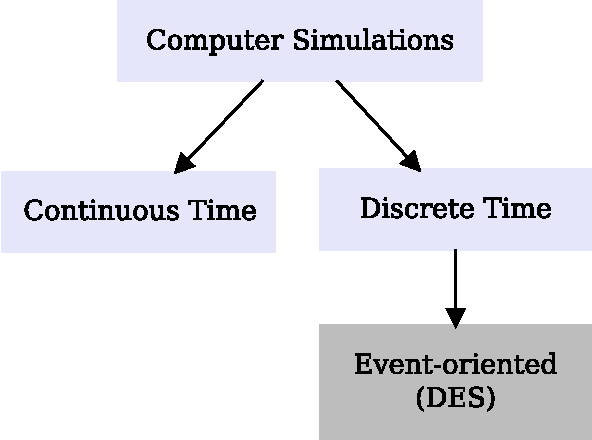
\includegraphics[width=0.5\textwidth]{figures/des.pdf}
    \caption{Discrete Event Simulation}\label{fig:des}
\end{figure}

A \emph{Discrete Event Simulation} model consists of three main data structures, namely:

\begin{description}

\item[Simulation clock:] that records the simulated time of the model under study.  This clock can be used for
  two primary purposes:
  \begin{itemize}
  \item measuring the progress of the simulation, and
  \item determining the order of events to be processed.
  \end{itemize}
  
\item[State variables:] The snapshot of the simulated system at any specific point in time (otherwise called
  state) can be described accurately by these set of variables.
  
\item[Pending event set:] A set of events that are yet to be processed.

\end{description}

\noindent
A physical system can be described by a set of physical processes grouped together to form a \emph{Simulation
  Model}.  Each of these physical processes corresponds to a \emph{Logical Process} (LP).  The LPs communicate
among themselves using timestamped events.  The timestamp marks the simulation time used for ordering and
processing of events.  The state of the system is updated only when an event is processed.

A \emph{Sequential Discrete Event Simulation} is a type of simulation where events are globally sorted and
processed sequentially one at a time.  A list holds all the events that are waiting to be processed and sorts
them in increasing order of timestamp.  The event with the lowest timestamp is processed first.  The state of
the system is updated and the simulation clock advances every time an event is processed.  It is also likely
that one or more new events are produced when an event is processed.  This sequential mechanism is too slow
and inefficient for large simulations and can be improved with parallelization.

\section[\textsc{pdes}]{Parallel Discrete Event Simulation}\label{sec:pdes}

The method for running a discrete event simulation on a parallel computing platform is called Parallel
Discrete Event Simulation (PDES).  The parallel computing platform can be a shared memory multiprocessor, a
distributed memory cluster, or a combination of both.  A synchronization mechanism is used to coordinate
parallel processing of events from different LPs while preserving the causal order for the final result
\cite{lamport-78}.  The \emph{Time Warp Mechanism} \cite{jefferson-85,fujimoto-90,fujimoto-00} is one such
synchronization mechanism that we will explore further in this dissertation.  It is an \emph{optimistic
  synchronization mechanism} which does not strictly preserve the causal order of events at all times and
sometimes temporarily allows violation by the simulation executive.  The next subsection provides a brief
overview of the Time Warp mechanism.

\subsection{Time Warp}\label{subsec:timewarp}

The Time Warp mechanism is an optimistic method of simulation.  It is based on the \emph{Virtual Time}
paradigm \cite{jefferson-85} which is a method for ordering events in distributed systems without requiring
any knowledge of real time. \emph{Virtual Time} is looked upon as the simulation time in case of parallel
discrete event simulation.

Events from different LPs can be processed independently in an optimistically synchronized mechanism such as
Time Warp.  No consideration is required for situations when lower timestamped events are received
\emph{i.e.,} when the causal order of event is violated.  Figure \ref{fig:causality_violation} depicts a
causality violation scenario by showing the timing diagram for events in three LPs.  An event with
\emph{timestamp = 3} is processed by $LP_1$ and two events are generated as a result, one with \emph{timestamp
  = 8} is sent to $LP_2$ and another with \emph{timestamp = 5} is sent to $LP_3$.  $LP_3$, on processing this
received event, generates an event for $LP_2$ with \emph{timestamp = 6}.  This event has a lower receive time
than the previous event (\emph{timestamp = 8}) received by $LP_2$.  If this previously received event is
processed by $LP_2$ before the event with lower receive time is received, it would lead to incorrect update of
the state as well as new events could be sent to itself or other LPs incorrectly.

\begin{figure}
    \centering
    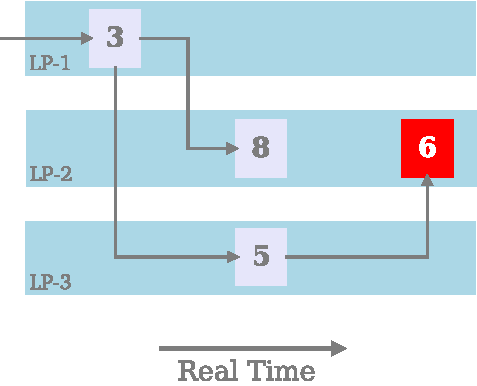
\includegraphics[width=0.4\textwidth]{figures/causality.pdf}
    \caption{Violation of Event Causality}\label{fig:causality_violation}
\end{figure}

\emph{Rollback} is the process of undoing the effects of incorrectly processed event(s) when a causality
violation is detected at an LP\@. \emph{Straggler event} is that incoming event with a timestamp lower than
the LP simulation clock (the LP has advanced prematurely).  The straggler event denotes a causality violation
and triggers a rollback.  According to Jefferson \cite{jefferson-85}, three data structures per LP are
necessary to handle rollbacks: \begin{inparaenum} [(1)] \item Input Queue, \item Output Queue, and \item State
  Queue\end{inparaenum}.  Figure \ref{fig:lp_data_structures} shows the Input Queue which contains all past
  and future event, the Output Queue contains all previously sent events, and the State Queue holds snapshots
  of previous states.

\begin{figure}
    \centering
    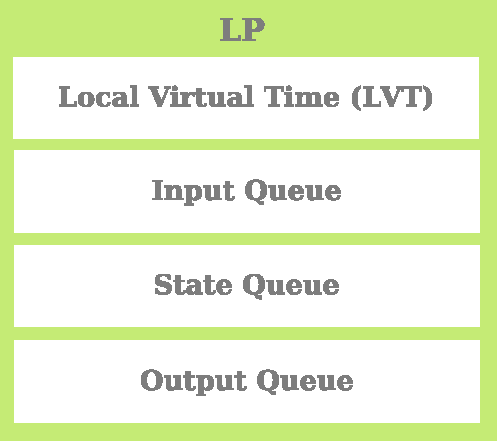
\includegraphics[width=0.4\textwidth]{figures/lp_data_structures.pdf}
    \caption{Data Structures of Logical Process in Time Warp}\label{fig:lp_data_structures}
\end{figure}

On rollback, the state of an LP is restored back to a snapshot that was saved at a timestamp prior to the
straggler event's receive time.  The Output Queue keeps track of all events, with send time greater than the
straggler event, that were sent incorrectly.  Those events are are re-sent but this time as an
\emph{anti-message} or \emph{negative event}.  An anti-messages is a copy of the positive event that has
already been sent, but with a crutial differentiator --- a bit within the event payload is set to indicate it
is a negative event.  The receiving LP does not process an anti-message in the same way as it processes a
positive event.  The anti-message's job is to cancel out the positive counterpart in the input queue.  The
anti-message can also be a straggler if it causes causality violation for the receiving LP.  In that scenario,
a rollback is triggered in the manner mentioned above.  This recursive process stops when the simulation is
rid of causality violations.

The minimum timestamp of all unprocessed events and anti-messages at any given point during the simulation is
called the \emph{Global Virtual Time} (GVT) of the simulation.  Events that have been sent but not yet
received are also tracked for this metric \cite{fujimoto-94}.  Timestamp of the smallest unprocessed event in
an LP is referred to as its \emph{Local Virtual Time} (LVT).  Though irrelevant as a metric on its own,
\emph{LVT} is essential to determine the \emph{GVT} in a distributed environment.  \emph{GVT} calculation is a
complex problem of estimation.  Several algorithms for GVT estimation have been discussed in \cite{weber-16}.
Estimation of \emph{GVT} allows us to fix a lower bound on how far back in time a rollback can occur.  This is
useful for selective elimination of events from the input and output queues and the states from the state
queue.  Only those events and states that have timestamp lower than GVT are eliminated since those will never
be used again.  This step is useful for memory reclamation as well as to commit I/O operations that cannot be
undone.  The process is called \emph{fossil collection} and it does not necessarily have to be GVT-based.
There are several other methods of fossil collection as discussed in \cite{weber-16}.

\section[\textsc{architecture}]{Architecture of Parallel Processing Systems}\label{sec:parallel_processing_architecture}

Parallel processing systems \cite{culler-97,patterson-11} are generally characterized based on the manner
in which processors and memories are grouped together.  A single machine which shares a common address
space for all processes is called a \emph{shared memory} system.  These systems can either have a single
physical memory unit or multiple memory units.  Multiple machines with separate process address connected
over interconnected network is called a \emph{clustered system}.

\subsection{Shared Memory Multiprocessors}\label{subsec:shared_memory_multiprocessors}

\paragraph{Symmetric Multiprocessor (SMP)} consists of a group of identical processing cores connected to a
single shared memory with full access to the input/output devices in the system.  This arrangement allows
uniform time access to the shared memory from each core.  In general, this architecture fails to scale up
linearly with increasing core counts due to the steep increase in memory contention.  As a results, the number
of processor cores in these configurations is generally bounded by some small number (generally $\leq$ 16,
although this number continues to increase).  Figure \ref{fig:smp} illustrates a typical \emph{SMP} system.

\begin{figure}
    \centering
    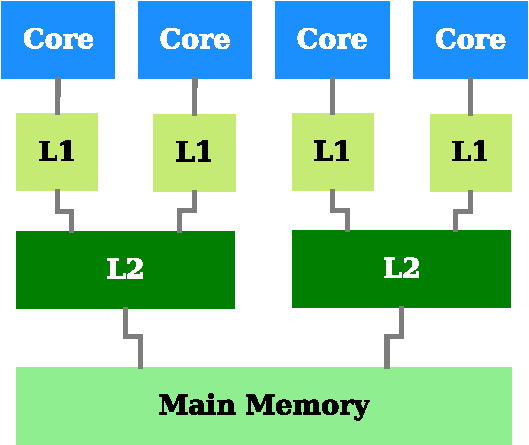
\includegraphics[width=0.45\textwidth]{figures/smp.pdf}
    \caption{A Symmetric Multiprocessor}\label{fig:smp}
\end{figure}

\paragraph{Non-Uniform Memory Access (NUMA)} processor has multiple cores and multiple memories with variable
access times to different memory locations based on the transport path between the processing cores and the
memory module.  In general, each core has a local memory module that provides fast access to its contents
while access to a non-local memory module (generally local to some other core) is accessed with a longer
access time.  Due to the higher access time for remote memory units, the common programming practice is to
maximize local memory accesses for a processor.  Compared to \emph{symmetric multiprocessors}, contention to
single memory does not necessarily increase when number of processors is increased in \emph{NUMA} systems.  As
a result, the latter system is capable of larger scale-up than SMP systems.  Figure \ref{fig:numa} illustrates
a typical NUMA system.

\begin{figure}
    \centering
    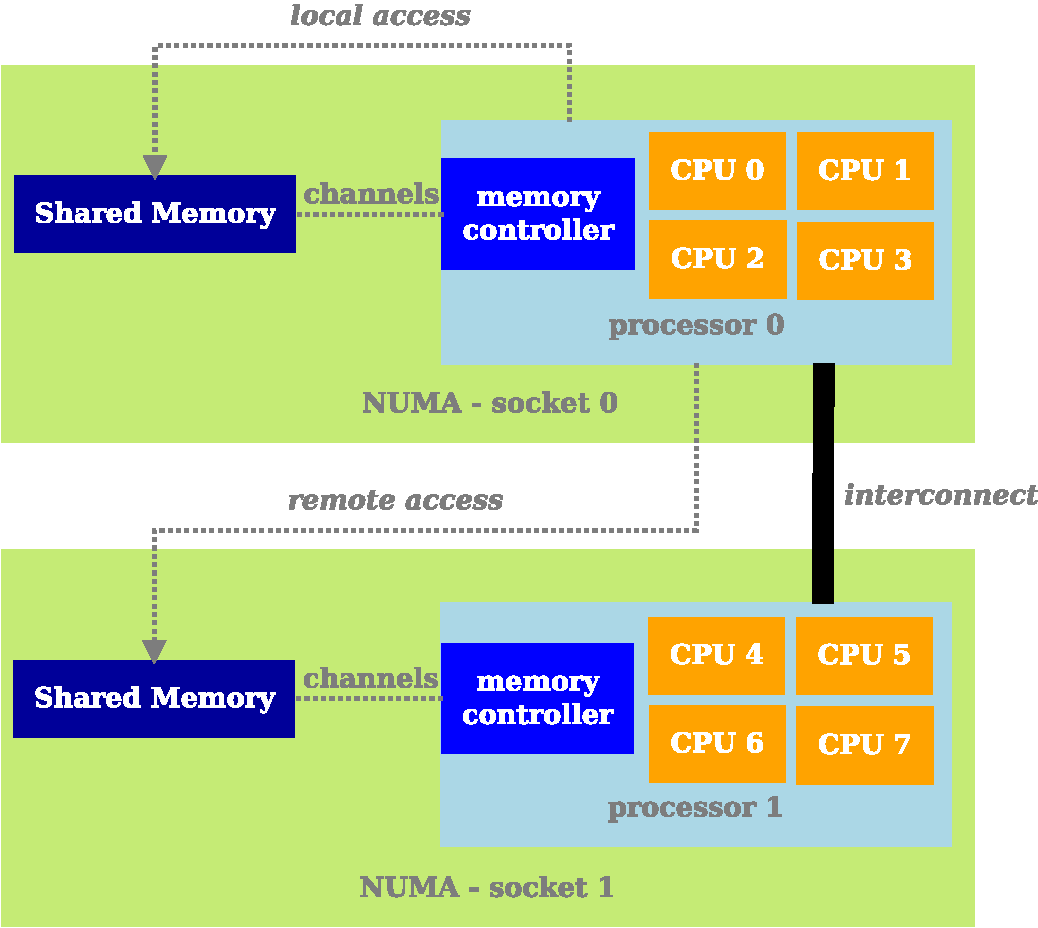
\includegraphics[width=0.75\textwidth]{figures/numa.pdf}
    \caption{A Non-Uniform Memory Access System}\label{fig:numa}
\end{figure}

\subsection{Clustered Systems}\label{subsec:clustered_systems}

A \emph{Beowulf Cluster} (or simply cluster) is a loosely coupled set of machines (also called nodes)
connected together over a local network.  It is designed to appear as a single machine to the user.  All nodes
on the cluster execute the same program concurrently by launching multiple processes on each machine.  A
cluster allows the program currently being processed to communicate among processes using some type of message
passing.  This message passing is generally handled by a parallel communication software such as \emph{Message
  Passing Interface (MPI)} \cite{gropp-94} or \emph{Parallel Virtual Machine (PVM)} \cite{geist-94}.  Figure
\ref{fig:beowulf} illustrates a commonly used version of the \emph{Beowulf cluster}.

\begin{figure}
    \centering
    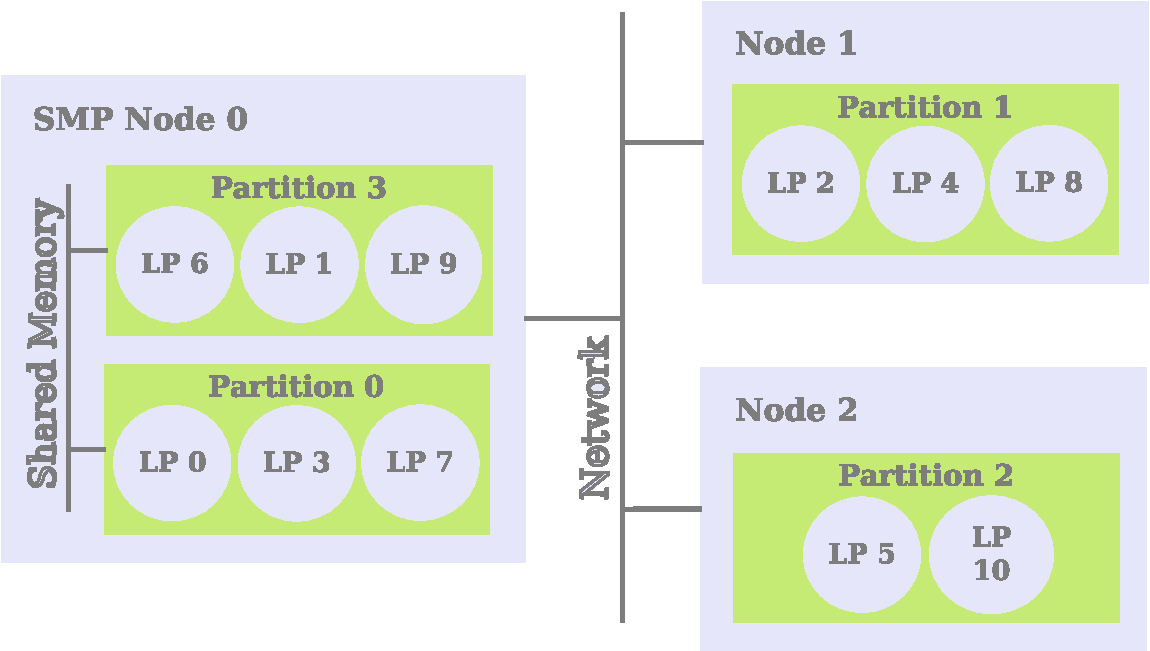
\includegraphics[width=0.75\textwidth]{figures/beowulf.pdf}
    \caption{Beowulf Cluster}\label{fig:beowulf}
\end{figure}

\section[\textsc{Communication}]{Communication in Parallel Systems}\label{sec:parallel_sys_comm}

Any application capable of parallel and independent execution on multiple processes/threads may
need to exchange information between these processes/threads.  Processes/threads can communicate
amongst themselves in either of these two ways:

\begin{itemize}

\item \emph{Message Passing}: explicitly pass messages to each other using well defined message formats, or

\item \emph{Shared Memory}: shared data structures accessible to all processes/threads.

\end{itemize}.

\noindent
There are fundamental differences between these two communication methods and both have their strengths and
weaknesses.  Sections \ref{subsec:msg_passing} and \ref{subsec:shared_memory} explore these two communication
models in further details.

\subsection{Message Passing}\label{subsec:msg_passing}

Processes communicate only through serialized messages in a message passing system.  These messages can be
passed either in \emph{synchronous mode} or in \emph{asynchronous mode}.  To enable the sender and receiver to
communicate via serialized messages, the format of the messages must be pre-defined.

\paragraph{Synchronous message passing} requires a specific ordering of the send/receive operations
for each process so that the sender/receiver processes can operate together in synchronized fashion.  Until a
message is received by the receiver, a sender's send operation will remain blocked.  Similarly, a receiver's
receive operation will remain blocked until the sent message is fully received.  These strict rules make every
process follow a predictable and synchronized communication pattern.  The whole system might suffer from a
slow down since processes are not allowed to execute other operations while communication operations are
ongoing.

\paragraph{Asynchronous message passing} allows processes to continue with routine executions
without blocking immediately after the start of send/receive operations.  All pending operations are held in
temporary queues and can be processed at any time and in any order.  As a result, these processes do not have
to follow a predictable communication pattern when communicating in asynchronous mode.

If the workload can be partitioned sensibly to keep remote communication at a minimum, the number of
cooperating processes can be scaled to essentially any size.  This is the chief advantage of \emph{message
  passing}.  These processes can utilize separate address spaces on different machines while communicating
over the local network.  However, it takes time to serialize, deserialize, and copy messages.  This latency is
significantly higher when compared to the processing speed of modern processors.  This latency is the chief
disadvantage of remote messaging.  There might be further delays when processes use an interconnection network
because of extra communication latency.  Fine-grained parallel applications need to send and receive lots of
small messages which is not something message passing is ideally suited.  Message passing is illustrated
in Figure \ref{fig:message_passing}.

\begin{figure}
    \centering
    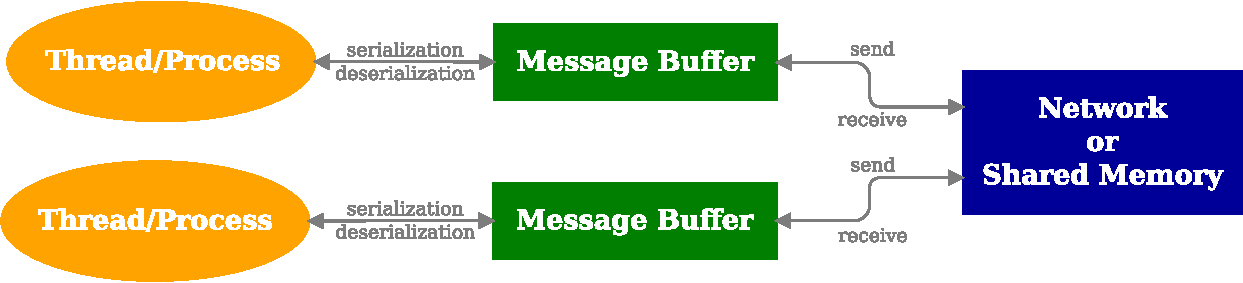
\includegraphics[width=0.9\textwidth]{figures/message_passing.pdf}
    \caption{Message Passing Communication Model}\label{fig:message_passing}
\end{figure}

\subsubsection{Message Passing Interface (MPI)}\label{subsec:mpi}

\emph{MPI} \cite{gropp-94} is an extensive and popular message passing standard popularly used for parallel
applications.  It supports both synchronous and asynchronous forms of communication and is a standard
specified for developers and other MPI users.  Several implementations of the MPI library exist, most popular
among them being \emph{MPICH} and \emph{OpenMPI}.

\subsection{Shared Memory}\label{subsec:shared_memory}

In parallel applications, it is possible for processes to communicate via shared data structures and share a
common address space.  A producer can be allowed to insert data directly into the data structures of a remote
machine and the consumers can then remove this data for usage.  Compared to message passing schemes, data
transmission via this shared data structure scheme takes less time.  Pointers can be also be used instead of
copying large datasets to further improve the speed.  To prevent multiple processes from corrupting the stored
data by simultaneously performing read-modify-write operations on the same data, access to the shared data
structures is protected usually using lock synchronization mechanisms.  Locks protect entire sections of code
that are executed by different processes when accessing the same data structures such as mutexes or
semaphores.  If too many processes contend for the lock simultaneously, the performance of shared memory data
structures may be adversely affected.  This makes it difficult to scale systems that use shared memory only as
means of communication. A simple shared memory system is illustrated in Figure \ref{fig:shared_memory}.

\begin{figure}
    \centering
    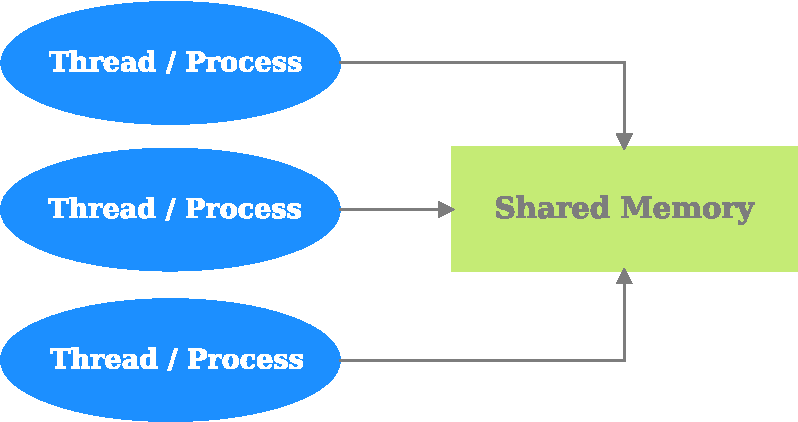
\includegraphics[width=0.55\textwidth]{figures/shared_memory.pdf}
    \caption{Shared Memory Communication Model}\label{fig:shared_memory}
\end{figure}

\chapter{Related Work}\label{chapter:related_work}

There are several popular implementations of Time Warp synchronized parallel simulation engines.  An overview
of some of the most popular ones is presented in this chapter.

\section{Georgia Tech Time Warp (GTW)}

Georgia Tech Time Warp \cite{das-94} (GTW) is a general purpose Time Warp Simulator that is not used anymore.
However, it is significant in that it was one of the most popular shared-memory PDES engine available.  The
shared memory multiprocessors such as the SparcStation and SGI PowerChallenge that \emph{GTW} was designed for
are now obsolete.  Inspite of being out-dated, \emph{GTW} set the template for most modern Time Warp
simulators in use today.  A single multi-threaded process runs a simulation model in \emph{GTW}.
Communication between threads is handled via shared data structures bound to a single processor.

A thread processes events from a statically allocated LP group in a simulation model.  This ensures that the
same processing core is used for processing events from a LP.  Each thread has its own set of data structures
to manage the distributed pending event set for its assigned LP group.  The pending event set for each
processor consists of three main data structures listed below \cite{das-94}:

\begin{enumerate}

\item \emph{Message Queue} is a linked list that holds positive messages for LPs.  Each message is mapped to
  the processor that handles that LP\@. Tasks running on any processor can access this shared data
  structure.  Access is usually synchronized via lock.

\item \emph{Cancel Queue} is similar to \emph{Message Queue} but, instead of positive messages, it holds
  negative messages (also known as anti-messages).  This queue also requires a lock for synchronized access.

\item \emph{Event Queue} is a composite data structure that is used to directly schedule events for
  processing.  It holds both unprocessed and processed events.  The event queue consists of two data
  structures, one each for processed and unprocessed events.  A doubly linked list holds the processed events
  while a priority queue holds the unprocessed events.  The priority queue can be configured by the user to be
  either a calendar queue or a skew heap.

\end{enumerate}

\noindent
Positive messages sent between LPs are inserted directly into the \emph{Message Queue} while negative ones are
directly inserted into the \emph{Cancel Queue}.  In order to process events, each thread first moves events
from the \emph{Message Queue} to the \emph{Event Queue} and then processes the rollbacks.  Messages from the
\emph{Cancel Queue} are removed next for event cancellations and any associated rollbacks are processed.  The
thread then processes one or more of the smallest events from the \emph{Event Queue} and adds those events to
the processed event list.  The procedure mentioned above is repeated by all processors until the end of the
simulation.  Figure \ref{gtw_processing} presents the pseudo-code for \emph{GTW's} main event processing loop.

\begin{algorithm}
\DontPrintSemicolon
    \While{Event Queue is not empty} {
        Transfer messages from Message Queue to Event Queue\;
        Process any rollbacks\;
        Remove anti-messages from Cancel Queue\;
        Cancel events and process associated rollbacks\;
        Remove one or more smallest events from unprocessed event pool in Event Queue\;
        process those events and move them to processed event pool\;
    }
\caption{Event Processing in GTW\cite{das-94,fujimoto-94}\label{gtw_processing}}
\end{algorithm}

Threads can remove multiple events from the \emph{Message Queues} and \emph{Cancel Queues} in order to avoid
frequent contention for access to these queues.  This type of processing is called batch processing and the
number of events in any batch represents the batch interval.  All events in a batch are processed serially
without consideration for rollbacks or cancellations.

In \emph{GTW}, there is no need to send anti-messages explicitly since all communication is over shared
memory.  \emph{GTW} calls its cancellation method \emph{direct cancellation} because only a pointer to the
event is needed for event cancellation.  GVT calculation also becomes faster on a shared memory platform since
shared data structures can be used more effectively instead of messages passed between processors.  This
approach, however, limits the use of \emph{GTW} to only a single multiprocessor machine, that too optimized
for specific architectures.

The developer of a simulation model is responsible for partitioning the LPs among processors.  This
partitioning must be done during initialization of the simulation model.  This is an unreasonable expectation.
To effectively partition the LPs, the model developer would need to understand some the features of the
underlying architecture such as the number of processors.  Additionally, this static partitioning approach
does not allow dynamic run-time balancing as there are no separate input queues for each LP\@.  All
unprocessed events for each processor are held within a single message queue.

\section{Clustered Time Warp (CTW)}

Clustered Time Warp \cite{avril-95} (CTW) employs a novel hybrid approach to processing events in
\emph{clusters}.  Events within a LP group (or \emph{cluster}) are processed sequentially while
synchronization between different clusters is via the Time Warp mechanism.  CTW was developed primarily to
support digital logic simulation.  Digital logic simulation tends to have localized computation within LP
groups and is suited for the computational framework of \emph{CTW}\@.  In addition, some simulation models
such as digital logic have events with fine computational granularity and lots of LPs.  In a Time Warp
simulator, this can cause significant increase in rollback count and memory footprint.  Although \emph{CTW}
supports shared memory multiprocessors, it only uses shared memory with a custom message passing system.
Thus, \emph{CTW} is best suited for NUMA architectures and is not recommended for execution on a Beowulf
Cluster.

Each LP cluster contains a timezone table, an output queue, and a set of LPs.  Each LP has an input queue and
a state queue.  Based on events received from different LP clusters, the timezones (and timestamps) are
recorded in the timezone table.  A new timezone is added to the timezone table when an event is received from
a remote cluster.  Since anti-messages can only be sent between clusters and between LPs inside a cluster, a
single output queue per cluster is sufficient.

\emph{CTW}'s rollback scheme is called \emph{clustered rollback}.  When a cluster receives a straggler event,
rollback will occur for all intra-cluster LPs that have processed events with timestamps greater than the
straggler event.  \emph{Local rollback}, which is an alternative to \emph{clustered rollback}, allows the
straggler event to be inserted into the input queue of the receiver LP\@.  The LP will trigger a rollback when
it detects this straggler event.  Even though \emph{clustered rollbacks} may slow down computation by
triggering rollbacks unnecessarily in some LPs, it eliminates the need to store processed events.  This
reduced memory footprint led \emph{CTW}'s designers to prefer \emph{clustered rollbacks}.

The timezone table in \emph{CTW} is used to determine the frequency of state savings.  Here the timezone of
the last processed event is looked up before processing an event.  The state is saved if this event belongs to
a different timezone.  This infrequent approach can broadly be classified into two categories, namely
\emph{local} and \emph{clustered} checkpointing.  In \emph{local checkpointing}, all LPs save their state
every time an event is processed in a new timezone, even if the event was received from a remote cluster.  In
\emph{clustered checkpointing}, only the LP that receives an event from a remote cluster saves its state. A
higher state saving frequency of the latter approach means more events must be saved for coast forwarding
during state restoration.  This increase in rollback computation and higher memory consumption was the reason
why \emph{CTW}'s designers preferred the \emph{local checkpointing} approach.

\section[\textsc{ross}]{Rensselaer's Optimistic Simulation System (ROSS)}

Rensselaer's Optimistic Simulation System (ROSS) \cite{carothers-00} is a general purpose simulator that
started life as a re-implementation of \emph{GTW}.  Its capabilities were enhanced steadily over the years and
now it can run both conservatively and optimistically synchronized parallel simulations as well as sequential
simulations.  It is widely used as a Timewarp-synchronized optimistic parallel simulator.

Although the event scheduling mechanism is similar to \emph{GTW}, \emph{ROSS} supports several priority queue
implementations.  There are also choices for algorithms used in fossil collection, state saving, and GVT
calculation.  A major difference between \emph{GTW} and \emph{ROSS} lies in the latter's use of processes
instead of threads.  \emph{ROSS} uses MPI-based message passing instead of shared memory for inter-process
communication.

\emph{ROSS}, borrowing ideas from \emph{GTW}, maps every LP to a process.  Each process contains its own
pending event set data structures and since these are not shared among processes, locks are unnecessary.
Although similar to the data structures in \emph{GTW}, \emph{ROSS} uses different naming convention as
mentioned below:

\begin{enumerate}

\item \emph{Event Queue} for a process holds all the positive events for all LPs linked to that process.  In
  addition, all remote events, both positive and negative, are held in the \emph{Event Queue}.  The structure
  is implemented as a linked list and is analogous to the \emph{Message Queue} in \emph{GTW}.

\item \emph{Cancel Queue} is similar to the data structure used in \emph{GTW} but without the lock (which is
  unnecessary here).  It is a linked list that holds negative events for all LPs for the corresponding
  process.

\item \emph{Priority Queue} holds events in increasing order of timestamp.  \emph{ROSS} allows the user to
  configure the type of implementation, options available are Calendar Queue \cite{brown-88}, heap
  \cite{williams-64}, Splay Tree \cite{sleator-85}, or AVL tree \cite{andelson-62}.  The \emph{Priority Queue}
  is analogous to the \emph{unprocessed event queue} in \emph{GTW}.

\end{enumerate}

\emph{ROSS} partitions the LPs on any process into groups called \emph{Kernel Processes (KPs)} in order to
reduce the time taken to fossil collect LPs.  Similar to \emph{clustered rollback} in \emph{CTW}, all LPs in a
\emph{KP} undergo rollback and fossil collection together.

Instead of relying solely on traditional copy state saving to rollback LPs to a previous state, 
\emph{ROSS} also uses \emph{reverse computation} \cite{carothers-99}.  

\subsection{ROSS-MT}

ROSS-MT \cite{jagtap-12} is a multi-threaded version of \emph{ROSS}.  Unlike the latter, \emph{ROSS-MT} is
optimized to use shared memory for inter-thread communication.  As message passing using MPI is completely
absent, all events are directly inserted into the \emph{event queues}.  \emph{Event Queues} are further
divided by possible senders in order to reduce the added contention on them.  The memory management in
\emph{ROSS-MT} suits NUMA architecture.

\section{\textsc{warped}}

\textsc{warped} \cite{martin-96,ramanan-98-iscope} is a general-purpose discrete event simulator.  It follows
Jefferson's classic model unlike the Time Warp simulators that came before it.  Here each LP has its own
input, output, and state queues.  \textsc{warped} was initially a process-based solution with communication
via message passing only.  With the development of multicore processors, in order to improve concurrent
processing of events, each process was extended into multiple threads.  The complexity of \textsc{warped}
became unmaintainable after few years because multiple researchers kept adding new features and algorithms to
it.  Though configurable and modular in design, \textsc{warped} became too complex for new developers to learn
and enhance.

This has led to the development of \textsc{warped2}, which is based on the design and architecture 
of \textsc{warped}. Chapter \ref{chapter:warped2_overview} provides a detailed overview of
\textsc{warped2}.

\section[\textsc{root-sim}]{The ROme OpTimistic Simulator (ROOT-Sim)}

The ROme OpTimistic Simulator \cite{pellegrini-11} (ROOT-Sim), a general purpose Time Warp simulator,
shares several common characteristics with \textsc{warped}.  Both use MPI-based message passing and can be
classified as classic Time Warp implementations since each LP has its own \emph{input}, \emph{state} and
\emph{output} queues.  ROOT-Sim is distinctly different from other Time Warp simulators when it comes to
internal instrumentation.  Memory usage can be optimized using \emph{Dynamic Memory Logger and Restorer
  (DyMeLoR)}.  \emph{DyMeLoR} analyzes the performance of simulation models to understand which is a better
fit --- \emph{copy-state saving} or \emph{incremental state saving}.  It can also transparently make a runtime
switch between these two state savings strategies.

Committed and Consistent Global Snapshot (CCGS) is a service that ROOT-Sim introduced for transparently
rebuilding the global snapshot of all LP states after each GVT calculation.  During every GVT calculation,
each LP has access to its portion of the global snapshot.  This service allows any simulation model to
implement its own custom global snapshot algorithm.

\emph{ROme} simulator does not advocate the use of shared memory event processing pool for the threads on an
SMP node\cite{vitali-12a,vitali-12b}.  Instead, it relies heavily on a partitioned pending event structure
with dynamic thread count in each kernel instance.  Depending on the current workload, the number of threads
can be scaled up or down.

In some of their recent papers \cite{marotta-16a,marotta-16b,ianni-17,marotta-17}, they have explored how all
threads can fully share the workload of events by loosely coupling simulation objects and threads.  Though
this fully shared pending event pool will allow concurrent processing of any event, it is necessary to design
parallel ``insertion'' and ``dequeue'' operations that are efficient.  Loosely based on the Calendar Queue
\cite{brown-88}, they claim that this scalable lock-free event pool is accessible concurrently with
\emph{O(1)} amortized time complexity for both ``insert'' and ``dequeue'' operations.

Speculative processing and rollback techniques are currently used for \emph{causality maintenance} by several
Time Warp-based PDES systems.  Pellegrini \emph{et al} \cite{pellegrini-17} question the effectiveness
of this approach and propose an alternative preemptive approach which requires the CPU to be dynamically
reassigned to past unprocessed events (or operations such as \emph{rollback}). According to the results they
present, this approach allows the simulation to deviate less from the critical path by reacting promptly to
the causal violations.  This reduces the overall number of \emph{causality violation} and is ideal for
multi-core \emph{x86-64} platforms.

\chapter[\textsc{warped2}]{The \textsc{warped2} Simulation Kernel}\label{chapter:warped2_overview}

\textsc{warped2} is a C++-based Time Warp synchronized parallel discrete event simulation kernel.  It is
extensively used for research on parallel simulations on multi-core processors and clusters.  The kernel also
provides a complete set of APIs that anyone can use to construct a simulation model.  However, a fair amount
of knowledge about Time Warp concepts is necessary at the beginning due to the low-level nature of some of the
APIs (\emph{e.g.,} state definition and copy constructors for the state).  The \textsc{warped2} kernel and
model git repositories are publicly available at \url{https://github.com/wilseypa/warped2} and
\url{https://github.com/wilseypa/warped2-models}. \textsc{warped2} supports two types of simulation, namely:

\begin{itemize}

\item sequential simulation, and 

\item Time Warp synchronized parallel simulation.

\end{itemize}

\section{Conceptual Overview}\label{sec:conceptual_overview}

In order to make \textsc{warped2} easy to configure, extend and maintain, the simulation kernel uses a modular
design.  At startup, all components are configured and created individually.  The sub-components are accessed
through pointers.  The kernel's event dispatcher supports both \emph{Sequential} and Time Warp
simulation.  Sequential simulator is a fairly simple software as it contains only a single list of unprocessed
events and does not require integration of any other component.  On the other hand, the Time Warp event
dispatcher requires integration of several components.  Each component provides specialized algorithms that
deals with one of the following:

\begin{itemize}
    \item event scheduling
    \item state saving
    \item cancellation
    \item GVT
    \item termination
    \item interprocess communication
    \item statistics
\end{itemize}

\noindent
Figure \ref{fig:warped2_architecture} illustrates the \textsc{warped2} implementation of Time Warp.

\begin{figure}
    \centering
    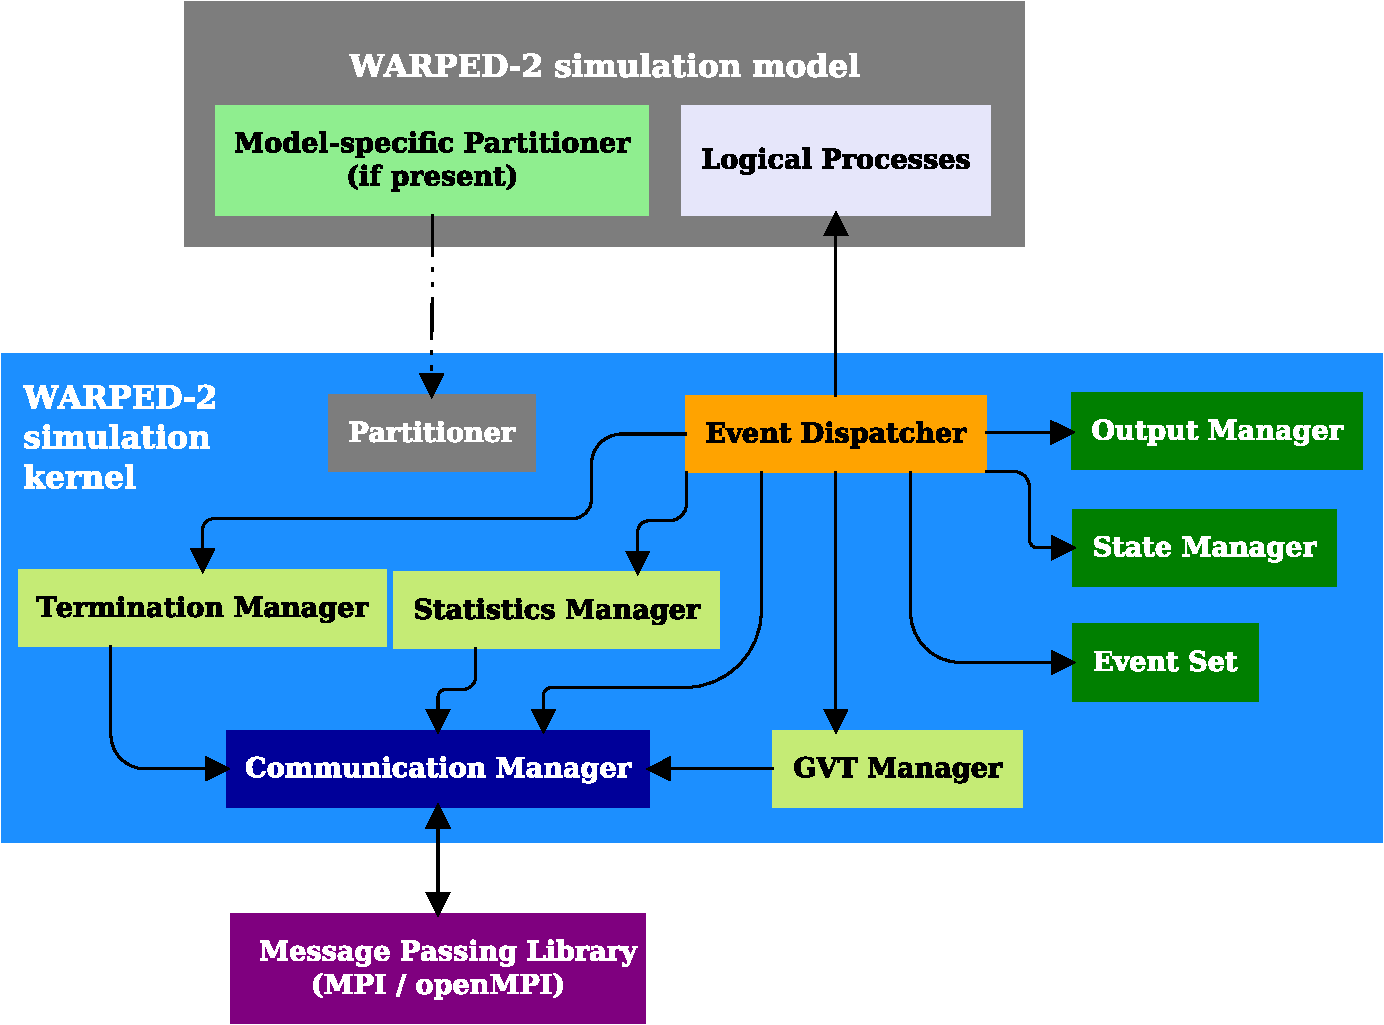
\includegraphics[width=0.9\textwidth]{figures/warped2_architecture.pdf}
    \caption{Time Warp Components in \textsc{warped2}}\label{fig:warped2_architecture}
\end{figure}

The components in Time Warp can be broadly classified as either \textbf{local} or
\textbf{global}. \emph{Local} components are responsible for controlling the node-specific
activities of all LPs on that node, namely event processing, rollbacks and fossil collection.
\emph{Global} components, on the other hand, are responsible for cluster-wide control
issues such as GVT, termination detection and calculation of statistics.  Communication to all
processes in a cluster environment is essential for determination of global state of the
system.

\subsection{Local Time Warp Components}\label{subsec:local_comporents}

The principle local components of \textsc{warped2} are:

\begin{itemize}

\item The \textbf{Event Set} contains all \emph{unprocessed} and \emph{processed} events for the LPs on a
  node. The important data structures include:
    
  \begin{itemize}
  \item \emph{Input Queue} for each LP, and 
  \item \emph{Schedule Queue} for events waiting to be processed soon.
  \end{itemize}
    
  \noindent
  The \emph{Event Set} is responsible for storage and scheduling of unprocessed events for execution.  It also
  processes rollbacks, and takes care of fossil collection for processed events.  The \emph{Event Set} has
  been designed for a multi-threaded environment and so the data structures that store pending events are
  designed for thread-safe concurrent or serialized access.

\item The \textbf{Output Manager} is the module that holds all the \emph{Output Queues} necessary for storage
  and tracking of outgoing events.  \textsc{warped2} supports only \emph{aggressive cancellation}
  \cite{fujimoto-90}.  The \emph{Output Manager} allows the kernel to do the following:
    
  \begin{itemize}
  \item add newly generated events to its output queues,
  \item dequeue events from output queues for processing a rollback, and 
  \item fossil collection of old output events to free up space on the output queues.
  \end{itemize}
  
\item The \textbf{State Manager} is the module that holds all the saved \emph{LP states} inside its state
  queues.  \textsc{warped2} supports only \emph{periodic state saving} \cite{fleischmann-95}. The \emph{State
    Manager} allows the kernel to do the following:
    
  \begin{itemize}
  \item saving the state of an LP,
  \item restore the state of an LP in case of a rollback, and
  \item fossil collection of old states in order to free up space in the state queues.
  \end{itemize}

\end{itemize}

\subsection{Global Time Warp Components}\label{subsec:global_componenets}

The major global components of \textsc{warped2} are:

\begin{itemize}

\item The \textbf{GVT Manager} is the module responsible for tracking the global progress of any simulation.
  The progress of a simulation is measured in terms of \emph{Global Virtual Time (GVT)} which can be
  calculated using either shared memory or message passing algorithms
  \cite{mattern-93,bellenot-90,fujimoto-94}.  In \textsc{warped2}, the GVT is calculated via a hybrid
  approach:

  \begin{enumerate}

  \item [Step 1:] multiple worker threads on each node regularly report the lowest timestamp for that node,
    and

  \item [Step 2:] nodes communicate their locally calculated lowest timestamp to other nodes for computation
    of the global progress as a minimum of these reported timestamps.

  \end{enumerate}
    
  \noindent
  \textsc{warped2} currently supports the following two GVT calculation modes:

  \begin{itemize}
  \item Synchronous \cite{fujimoto-94} mode focuses on synchronized global reduction between all threads from
    all processes, and 
  \item Asynchronous \cite{mattern-93} mode uses Mattern's message passing algorithm \cite{mattern-93} and
    Fujimoto's shared memory algorithm \cite{fujimoto-94}.
  \end{itemize}

  \noindent
  A more detailed explanation of the GVT algorithms of \textsc{warped2} are available in \cite{weber-16}.

\item \textbf{Termination Manager} is the module in \textsc{warped2} that initiates termination when it
  realizes all processes in the simulation have become inactive.  Similar to the \emph{GVT Manager}, the
  \emph{Termination Manager} requires a hybrid approach involving worker threads and \emph{Communication
    Manager}.

\item \textbf{Statistics Manager} records local statistics on a distributed simulation.  It also provides
  reduction methods to allow \textsc{warped2} use the local statistics to compute and report consolidated
  statistics for the whole simulation.

\end{itemize}

\subsection{Communication Manager}\label{subsec:communication_manager}

The \emph{Communication Manager} is the module that facilitates connection between the global Time Warp
components and the underlying message passing library.  In \textsc{warped2}, the entire interprocess
communication, including remote events sent to or received from another process, is channeled through the this
Communication Manager.  The manager accepts registration from any class that needs interprocess communication.
This registration requires the class to inform the message type and provide a callback function for receiving
events.

\subsection{Partitioner}\label{subsec:partitioner}

The \emph{Partitioner} is a module responsible for dividing the logical processes of a simulation into groups
(or partitions).  At the time of initialization, the \emph{Partitioner} is asked to create a defined number of
partitions from a provided list of LPs using a partitioning technique.  The \textsc{warped2} kernel provides
support for the following types of partitioning strategies:

\begin{itemize}

\item \emph{Round Robin} partitioning is cyclic binning of LPs into different partitions.  Figure
  \ref{fig:round_robin} illustrates this algorithm.

\item \emph{Profile-Guided} partitioning is a network statistics driven partitioning strategy. Alt \emph{et
  al} \cite{alt-14} studied how this partitioning can be done to minimize the number of remote messages sent
  in a distributed environment. They presented data that showed the effectiveness of \emph{METIS}
  \cite{karypis-98} as an effective partitioning tool for the LPs. The \emph{profile-guided} partitioning in
  \textsc{warped2} is done by partitioning a weighted LP network graph using \emph{METIS}, where weight is the
  count of events (or messages) exchanged between any two LPs. Section \ref{subsec:bags} explains the
  \emph{event bag scheduling} technique which relies on \emph{modular communities} of LPs found by the
  \emph{Louvain} partitioning algorithm \cite{blondel-08}.
    
\item Users can define \emph{Custom} partitioning strategies to suit the needs for the simulation model they
  are building.

\end{itemize}

\begin{figure}
    \centering
    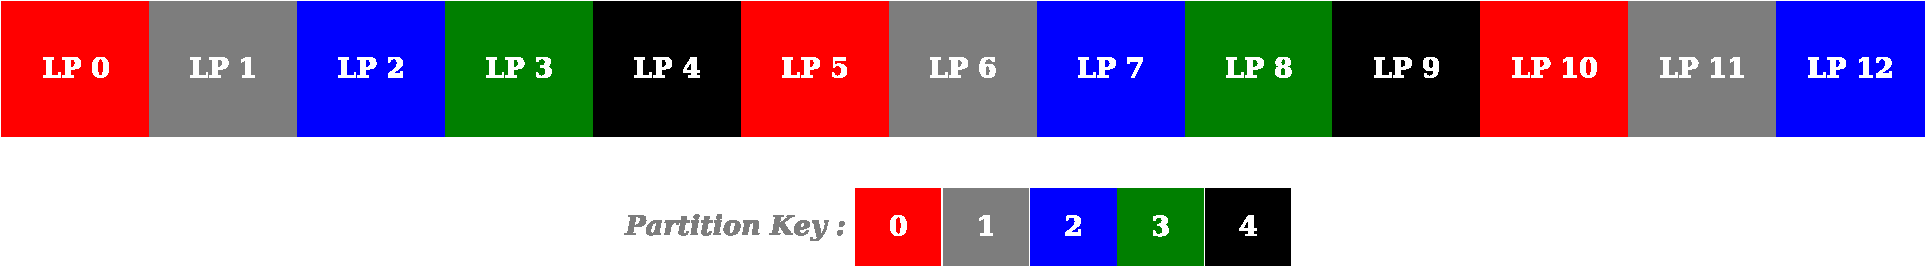
\includegraphics[width=1\textwidth]{figures/round_robin_partitions.pdf}
    \caption{Round Robin Partitioning in \textsc{warped2}}\label{fig:round_robin}
\end{figure}

\emph{Partitioning} is an effective way to distribute workload across a parallel computing platform,
especially if the simulation size is too large for any individual machine.  Figure \ref{fig:beowulf} shows how
different \emph{partitions} can be distributed on different nodes in a \emph{Beowulf cluster}.

\section{Journey of an Event}\label{sec:journey_of_event}

\subsection{How are Events Ordered?}\label{subsec:event_order}

The implicit assumption for Time Warp is that every event is tagged with a totally ordered clock value based
on virtual time \cite{jefferson-85}.  This is essential to ensure that results from different simulation runs
are deterministic \cite{ronngren-99}.  Having a global tag for each event ensures the preservation of causal
dependencies.

\noindent
In order to ensure total ordering of events, \textsc{warped2} uses the following 4-tuple scheme:

\begin{enumerate}
    \item Receive Timestamp
    \item Send Timestamp
    \item Name of Sender LP
    \item Generation
\end{enumerate}

\noindent
For practical purposes, the \textbf{Receive Timestamp} is the tagged clock value for each event.  In
situations where multiple events share the same \emph{Receive Timestamp} value, the last three event
parameters allow those events to be ordered.

\paragraph{Send Timestamp} for virtual time systems is analogous to Lamport's logical clock
\cite{lamport-78} in real time distributed systems.  It can ensure correct ordering of events as long as an LP
sends only one event with a unique combination of \emph{Send Timestamp}, \emph{Receive Timestamp} and
\emph{Receiver LP}.  Otherwise, strict ordering of events would not be preserved and \textsc{warped2} forbids
that.

\paragraph{Name of Sender LP} is necessary when \emph{Send Timestamp} fails to order all
events correctly.  Events received with the same combination of \emph{Receive Timestamp} and \emph{Send
  Timestamp} from different senders can be ordered using \emph{Name of the Sender LP}.  If this is not
implemented, it is possible to get different results from different runs of the simulation \cite{ronngren-99}.

\paragraph{Generation} is a per-LP counter that keeps track of the number of events sent
from a particular LP\@.  In distributed memory systems, this counter value helps to differentiate between the
same event which might get re-sent after a \emph{rollback} \cite{ronngren-99}.  Each event is tagged with a
\emph{Generation id} before being sent.  This value is then used at the receiver's end for resolving any
conflicts in the event order.

\subsection{Pending Event Set}\label{subsec:pending_event_set}

The set of events that are waiting to be processed is referred to as \emph{Pending Event Set}.  In
\textsc{warped2}, each process maintains a pending event set for its dedicated set of LPs.  This pending event
set is logically separate from that of other processes.  Events generated by a LP can either be sent
\emph{locally} to a LP present on the same process (or node) or can be sent to a LP on a \emph{remote}
process. \emph{Local events} are inserted directly into the pending event set while \emph{remote events} are
inserted into a \emph{remote event send queue}.  The \emph{manager thread} present on each process removes
these \emph{remote events} from the queue, forms \emph{event messages} and sends these messages to the
intended receiver process.  The \emph{manager thread} at the other end, on receiving an \emph{event message},
unpacks this message to re-form the event and then inserts this event into the \emph{pending event set} of the
receiver.  Each LP in the \emph{pending event set} has its own \emph{Input Queue} which temporarily holds all
incoming events for that LP till they are processed.  This queue is directly accessible to all threads and is
protected by a lock.

The \emph{Input Queue} holds both positive events and negative events (or anti-messages) and keeps all stored
events sorted in increasing order at all times.  In terms of sorting order, \emph{anti-messages} have priority
over their \emph{positive} counterparts.  This mechanism ensures \emph{anti-messages} are noticed first and,
while processing it, the positive counterpart (if present in the \emph{Input Queue}) can be \emph{cancelled}.
This helps to eliminate `preventable' rollbacks \cite{lubachevsky-89}.  The \emph{Input Queue} only stores
pointers to unprocessed events which ensures events are not unnecessarily copied.  Event data replication will
lead to an excessive use of available memory.

The \emph{Schedule Queue} is a secondary data structure that is part of \textsc{warped2}'s pending event set.
The original design of \textsc{warped2} assumes that this \emph{Schedule Queue} is a \emph{LTSF (Lowest
  TimeStamp First) Queue} (similar to an \emph{Input Queue}) because it sorts lowest timestamped events from
multiple LPs in increasing order.  One event from each LP is \emph{scheduled} into a common \emph{Schedule
  Queue}.  Scheduling an event here implies copying of event pointer into the \emph{Schedule Queue}.  The
event is not removed from the \emph{Input Queue} while it is \emph{scheduled}.  A worker thread ``dequeues''
the smallest event available in the \emph{Schedule Queue} for processing.  One or more \emph{Schedule Queues}
may be available for each process (or node).  Since multiple worker threads can access a particular
\emph{Schedule Queue}, access to this data structure is serialized using a lock.

For each LP, it is necessary to keep track of the event that has been scheduled for the following
reasons:

\begin{itemize}

\item It provides a way to identify whether the smallest event from an LP has been scheduled.  When an event
  is into the \emph{Input Queue} of an LP, it can be compared against the currently scheduled event.  If it
  turns out that the newly inserted event is smaller, the new event can then be scheduled in place of the
  already scheduled event.

\item It prevents multiple worker threads from processing events in the same LP.  This might lead to an
  undetected case of \emph{causality violation} causing out of order event commits to happen without
  corrections via rollback.

\end{itemize}

\noindent
Figure \ref{fig:timewarp_pending_event_set} depicts the pending event set data structures used in
\textsc{warped2}.

\begin{figure}
    \centering
    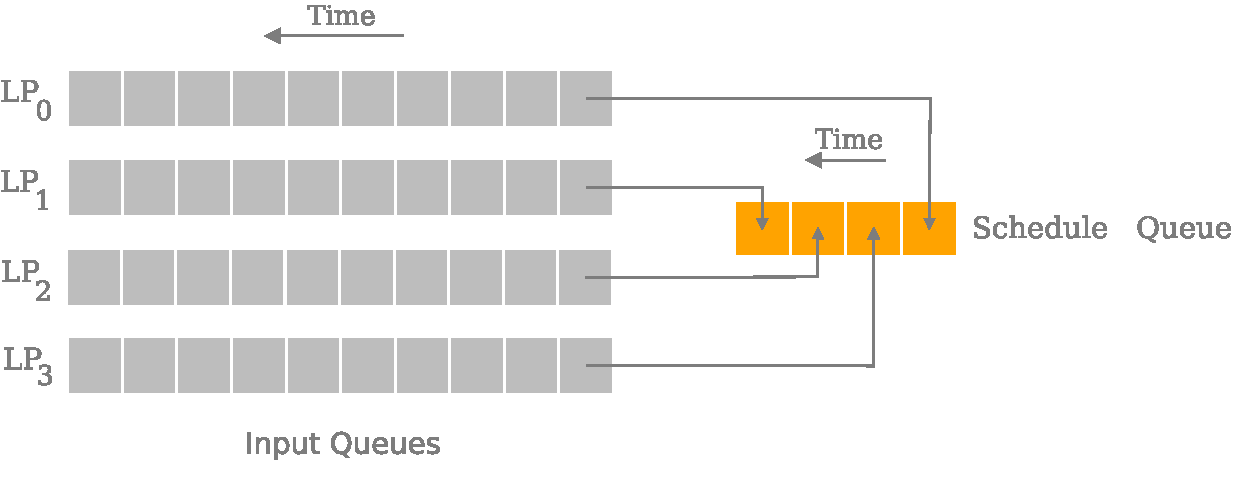
\includegraphics[width=0.9\textwidth]{figures/timewarp_pending_event_set.pdf}
    \caption{\textsc{warped2} Pending Event Set}\label{fig:timewarp_pending_event_set}
\end{figure}

\subsection{Processing of Events}\label{subsec:event_processing}

At the start of simulation, each \emph{Schedule Queue} is allocated one or more worker threads.  Each thread
processes events following the exact same procedure.  A scheduled event is ``dequeued'' from a \emph{Schedule
  Queue} but remains stored in the \emph{Input Queue} until that event has been either processed or cancelled
out.  In order to ensure the dequeued event is not a \emph{straggler}, it is first compared against the last
processed event for that receiving LP.  If it turns out to be a straggler, rollback procedure is initiated for
that LP.  A \emph{straggler} may also be an \emph{anti-message} if its \emph{positive} counterpart has already
been processed.  Due to the manner in which \textsc{warped2} cancels positive event in \emph{Input Queue} on
receiving an \emph{anti-message}, it can be assumed that if the scheduled event is an \emph{anti-message}, it
is a \emph{straggler} and the LP needs to rollback.  If the scheduled event is a positive one and not a
\emph{straggler}, then it is processed normally and the \emph{LP State} is saved.  Any new events that were
generated are sent to the intended LPs.  The recently processed event is then stored in the \emph{Processed
  Queue} and a new event is scheduled from the LP into the \emph{Schedule Queue}.  Algorithm
\ref{algo:event_loop} summarizes the worker thread event processing loop.  In general, the algorithm proceeds
as follows: before an event is inserted into the \emph{Input Queue}, it is compared to the event that is
currently scheduled for that LP.  The new event is immediately scheduled if the corresponding LP has currently
scheduled event or if the new event is smaller than the currently scheduled event.  This prompt initiative
prevents a rollback from occurring.

\begin{algorithm}
\DontPrintSemicolon
\SetKw{Continue}{continue}
\SetKwFunction{getNextScheduledEvent}{getNextScheduledEvent}

    \While{signal to terminate not detected}{
        $e \gets \getNextScheduledEvent{}$\;
        $LP \gets$ receiver of $e$\;\;

        \If{$e <$ last processed event for $LP$}{
            Rollback $LP$\;
        }
        \;
        \If{$e$ is an anti-message}{
            Cancel event with $e$ (if possible)\;
            Schedule new events for $LP$\;
            \Continue\;
        }
        \;
        Process event $e$\;
        Save state of $LP$\;
        Send newly generated events to their destinations\;\;

        Move $e$ to Processed Queue\;
        Replace scheduled event for $LP$ with an event from the Input Queue
        (if available)\;
    }

\caption{\textsc{warped2} Event Processing Loop}\label{algo:event_loop}
\end{algorithm}

\subsection{Rollbacks \& Cancellation}\label{subsec:rollbacks}

According to Jefferson \cite{jefferson-85}, three data structures are necessary for the rollback and event
cancellation process, namely: the \emph{Input Queue}, the \emph{Output Queue}, and the \emph{State Queue}.
The data structures used in \textsc{warped2} are based on Jefferson's description.  But while Jefferson's
approach requires the \emph{Input Queue} to hold both unprocessed and processed events, separate data
structures are maintained in \textsc{warped2} for ease of scheduling.

A 3-tuple value is stored for each entry in the \emph{State Queue}.  The tuple attributes are:

\begin{itemize}

\item The address of the memory location holding the saved copy of the LP state.
    
\item The address of event that produced the LP State.  If there is a rollback, this event will be compared
  against the straggler event for identifying the restore point.  It will also be compared against the GVT
  value during fossil collection.
    
\item In order to ensure deterministic results, state of the LP's random number generator is saved.  A linked
  list holds these states and are restored during a rollback.

\end{itemize}

\noindent
Each entry into the \emph{Output Queue} is a tuple similar to that in a \emph{State Queue}.
The tuple attributes are:

\begin{itemize}
\item address of the source event, and
\item address of the sent event.
\end{itemize}

\noindent
In order to figure out which sent events need to be cancelled out via anti-messages in case of a rollback, the
source event is compared against the straggler event. \emph{Processed Queue} of an LP holds the addresses of
events processed from that LP.

\chapter[\textsc{Pending Event Set}]{Optimizing \textsc{warped2}'s Pending Event Set}\label{chapter:event_scheduling}

This chapter is a continuation of the discussion on \emph{Pending Event Set} started in Section
\ref{subsec:pending_event_set}.  As mentioned in that section, the \emph{Schedule Queue} is a data structure
that stores lowest unprocessed pending events from all of the LPs in sorted order.  Worker threads contest for
dedicated access to this shared data structure in order to ``dequeue'' events for processing.  Conventional
designs visualize this \emph{Schedule Queue} as a priority queue where events are arranged in increasing order
of their timestamp.  However, in this chapter, alternative ideas on sorting data structures and scheduling
techniques will be presented to show it is not always necessary to fully sort all pending events.  The
remainder of this chapter is organized as follows.  Section \ref{sec:data_structures} presents the different
data structures that can be used as \emph{Schedule Queue} in \textsc{warped2}.  Section
\ref{sec:scheduling_techniques} presents some scheduling techniques which, when used in combination with the
data structures discussed in Section \ref{sec:data_structures}, can boost the performance of the
\textsc{warped2} simulator.

\section[\textsc{Data Structures}]{Data Structures for Scheduling Pending Events}\label{sec:data_structures}

Ronngren \emph{et al} \cite{ronngren-93} proposed that all unprocessed and processed events along with each
event's execution status can be stored inside a common data structure called \emph{Linear List}.  The
\emph{Linear List} is a doubly linked list \cite{newell-57} that is simple to implement.  Though rollbacks and
fossil collection become more efficient when using \emph{Linear List}, the authors \cite{ronngren-93} state
that \emph{Linear List} struggles to insert events into a large event pool.  As an alternative to linear list,
they suggest that the improved skew heap \cite{sleator-86} is a promising alternative.

Prasad \emph{et al} \cite{prasad-95a,prasad-95b} proposed that, for medium to coarse-grained simulations,
parallelized Calendar Queues \cite{brown-88} can be used.  Each processor maintains its own separate Calendar
Queue.  The result from their experiment showed that arranging the pending events into queues locally does not
adversely impact the balance of the simulator when compared to the standard global queue-based arrangement.

Santoro \emph{et al} \cite{santoro-10} proposed a modified version of the Calendar Queue that uses an array
and a hierarchical bitmap.  They show that this modification allows the priority queue to access its stored
events in constant-time with low overhead.

In \textsc{warped2}, several different data structures have previously been explored for managing the pending
event set.  Similar to the aforementioned research on priority queues, a reduction of the overhead involved in
sorting events remains a major motivating factor.  However, the advent of multi-core processors and the
subsequent analysis of the contention issues involved in using shared data structures has raised concerns
about the current design.  In Sections \ref{subsec:stl_multiset_splaytree}, \ref{subsec:ladderq},
\ref{subsec:unsorted_bottom} and \ref{subsec:lockfree} several different data structures are explored for
creating an effective \emph{Schedule Queue} in \textsc{warped2}.

\subsection{STL MultiSet and Splay Tree}\label{subsec:stl_multiset_splaytree}

The \emph{C++ STL MultiSet} and \emph{Splay Tree} are both well-known tree-based implementations of a priority
queue and are used extensively in different applications.  \emph{STL MultiSet} is a sorted multiple
associative container present in the Standard Template Library \cite{musser-89} which is similar to a
\emph{Set} container but, unlike the latter, allows multiple instances of any element.  It permits lookup,
insertion, and removal of an element in \emph{O(log n)} amortized time and is ideal for quickly verifying
whether an element is present inside the container. The STL MultiSet has been implemented using
\emph{Red-Black Tree} \cite{cormen-01}, a self-balancing binary search trees and supports bidirectional
iterators.

Similar to the \emph{STL MultiSet}, the \emph{Splay Tree} \cite{sleator-85} is also a variation of
self-adjusting binary search tree that allows for quick access to recently accessed elements.  It can insert,
lookup, and remove an element in \emph{O(log n)} amortized time.  The \emph{Splay Tree} used in
\textsc{warped2} is a faithful implementation of the original data structure described in \cite{sleator-85}.

\subsection{Ladder Queue}\label{subsec:ladderq}

The \emph{Ladder Queue} \cite{tang-05} is a priority queue which utilizes the bucket-based sorting philosophy
of a Calendar Queue \cite{brown-88}.  In case of a Calendar Queue, each bucket stores events within a certain
time-window (or month) and the entire data structure must sometimes be resized at regular intervals in order
to balance the changing range of event timestamp across the buckets.  The Ladder Queue avoids the need for the
resizing of buckets by dynamically splitting only the bucket with earliest event timestamps into multiple
buckets once the number of events stored in that particular bucket exceed a pre-defined threshold.  Figure
\ref{fig:ladderq_sorted} illustrates the principle components of a Ladder Queue.

\begin{figure}
    \centerline{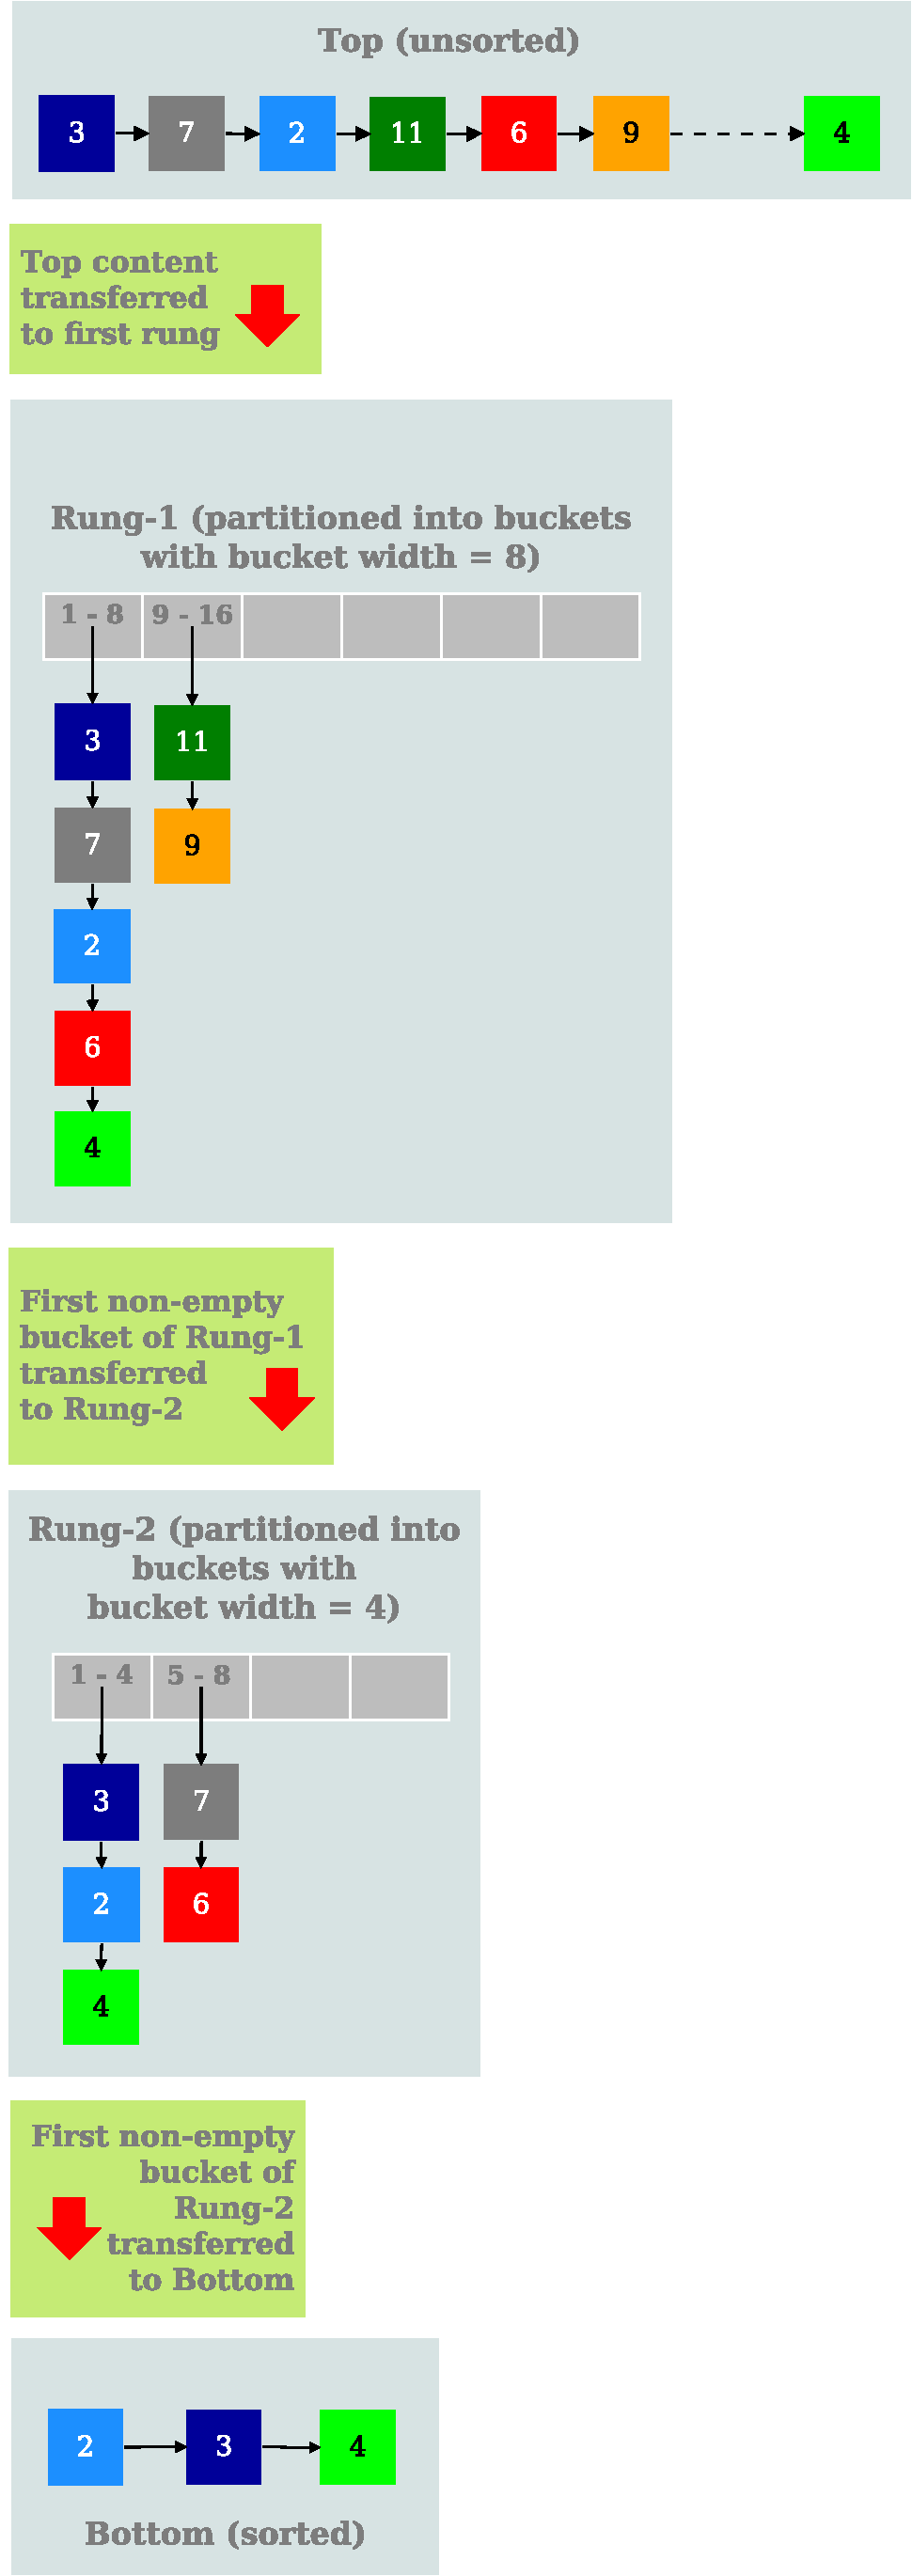
\includegraphics[width=0.41\textwidth]{figures/ladderq_sorted.pdf}}
    \caption{The Ladder Queue Structure}
    \label{fig:ladderq_sorted}
\end{figure}

Initially the Ladder Queue data structure is empty.  Incoming events are inserted into the \emph{Top}
structure without sorting.  The minimum and maximum timestamp values for events stored inside Top are updated
(if needed) when any new event is inserted there.  On receiving the first ``dequeue event'' request, the
events in Top are transferred to $Rung_1$.  The total bucket count in $Rung_1$ is configurable dynamically.
The time window of events transferred from Top is uniformly partitioned into all the buckets available in
$Rung_1$.  The buckets store events without sorting in $Rung_1$ and there is an upper threshold for the number
of events that can be stored in each bucket.  When the number of events in the first non-empty bucket of the
current rung exceed this threshold, a new lower rung is created.  Events from the first non-empty bucket are
then transferred to this new rung by splitting the bucket's time window uniformly across all buckets in the
new rung.  Figure \ref{fig:ladderq_sorted} illustrates how this process works.  Here events from the first
non-empty bucket in $Rung_1$ is transferred to $Rung_2$ by splitting the time window of the bucket uniformly.
Thus, the bucket size (defined as the number of elements in the bucket) of each bucket in $Rung_2$ is a
sub-range of the bucket size in $Rung_1$.

The final step in the ``dequeue event'' process is transfer of the first non-empty bucket (which holds events
with the smallest timestamps) to \emph{Bottom}.  The Bottom is a priority queue which sorts events in
increasing order of their timstamp.  The ``dequeue'' operation is then able to pull the smallest event stored
in Bottom.  Bottom then holds the smallest events available to the \emph{Ladder Queue}.  Events can be
dequeued from Bottom until it becomes empty.  Any new dequeue request at this point initiates another transfer
of events from the rungs.  The first non-empty bucket of the lowest available rung is transferred to the
Bottom.  When the events in the rungs and Bottom of the ladder are exhausted, these ladder elements are
replenished by transferring events from the Top.  Algorithm \ref{algo:ladderq_dequeue} explains how events are
dequeued from the Ladder Queue.

\begin{algorithm}
\DontPrintSemicolon
\SetKw{Return}{return}
\SetKwFunction{timestamp}{timestamp}
\SetKwFunction{minTS}{minTS}
\SetKwFunction{maxTS}{maxTS}
\SetKwFunction{bucketWidth}{bucketWidth}
\SetKwFunction{size}{size}

    \If{Bottom not empty}{
        event $e \gets$ dequeue event from head of $Bottom$\;
        \Return $e$\;
    }
    \;
    \If{Rung(s) exist}{
        Find first non-empty bucket $k$ in the lowest available rung $x$\;
        Transfer events from bucket $k$ in rung $x$ to $Bottom$\;
        Delete rung $x$ if it has no non-empty buckets left\;
        event $e \gets$ dequeue event from head of $Bottom$\;
        \Return $e$\;
    }
    \;
    \textit{/* Transfer events from Top into Rung(s) and Bottom */}\;
    \;
    $Rung[1].\bucketWidth \gets \frac{Top.\maxTS - Top.\minTS}{Top.\size}$\;
    \;
    $Rung[1].\minTS \gets Top.\minTS$\;
    Transfer $Top$ into $Rung[1]$\;
    $Top.\minTS \gets Top.\maxTS$\;
    Find first non-empty bucket $k$ in $Rung[1]$\;
    Transfer events from bucket $k$ in $Rung[1]$ to $Bottom$\;
    Delete $Rung[1]$ if it has no non-empty buckets left\;
    \;
    event $e \gets$ dequeue event from head of $Bottom$\;
    \Return $e$\;
    \;
\caption{\textsc{Ladder Queue} Dequeue Operation}\label{algo:ladderq_dequeue}
\end{algorithm}

After the initial events to the Ladder Queue are pulled from Top into the ladder rungs, any new incoming
events are inserted into that element of the Ladder Queue (Top, Rungs, or Bottom) based on the value of its
timestamp as consistent with the current timestamp ranges contained in those elements.  That is, if an event's
timestamp lies within the time window of any rung, it is inserted into a specific bucket on that rung; the
event is inserted into Bottom if the timestamp is lower than any of the available rungs; and finally any
incoming event with timestamp greater than $Rung_1$'s time window is inserted into \emph{Top}.  Algorithm
\ref{algo:ladderq_insert} explains the ``insert event'' operation in details.

\begin{algorithm}
\DontPrintSemicolon
\SetKw{Return}{return}
\SetKwFunction{timestamp}{timestamp}
\SetKwFunction{sizeThreshold}{sizeThreshold}
\SetKwFunction{minTS}{minTS}
\SetKwFunction{bucketWidth}{bucketWidth}
\SetKwFunction{size}{size}

    \If{$e\rightarrow\timestamp{} \geq Top.\minTS$}{
        Insert event $e$ into tail of $Top$\;
        \Return\;
    }
    \;
    \While{$e\rightarrow\timestamp{} < Rung[x].\minTS$}{
        x++\;
    }
    \;
    \If{$x \in$ valid rung}{
        \;
        bucket $k \gets \frac{e\rightarrow\timestamp{} - Rung[x].\minTS}{Rung[x].\bucketWidth}$\;
        \;
        Insert event $e$ into tail of bucket $k$ of rung $x$\;
        \Return\;
    }
    \;
    \If{$Bottom.\size > Bottom.\sizeThreshold$}{
        \;
        Create new rung whose index is $y$\;
        Transfer events from $Bottom$ to $Rung[y]$\;
        \;
        \textit{/* Insert event e into the Rung[y] */}\;
        \;
        bucket $k \gets \frac{e\rightarrow\timestamp{} - Rung[y].\minTS}{Rung[y].\bucketWidth}$\;
        \;
        Insert event $e$ into tail of bucket $k$ of rung $y$\;
        \Return\;
    }
    \;
    Insert event $e$ into $Bottom$\;
    \Return\;
    \;
\caption{\textsc{Ladder Queue} Insert Operation}\label{algo:ladderq_insert}
\end{algorithm}

\subsubsection{What is exciting about the Ladder Queue?}\label{subsubsec:why_ladder}

From a conceptual standpoint, the Ladder Queue is able to store events from different
\emph{epochs}\footnote{Each pull of events from Top into the Rungs and Bottom of the ladder queue is termed a
  new epoch.} separately in its different sub-structures.  Events from one epoch (whose timestamps fall in the
range $t$ and $t+\Delta t$) are held in the Bottom and Rung elements while events from the next epoch
(timestamps above $t+\Delta t$) are held in the Top element.  Any incoming event is inserted into one of these
three Ladder Queue elements based on its timestamp.  When there are no more events left inside Bottom and
Rung(s), a ``dequeue'' operation moves the ladder queue to its next epoch.  The events in Top are then
transferred to the Rung(s) and Bottom.  The time window of an epoch ($t$ to $t+\Delta t$) is defined by the
minimum and maximum timestamp of events pulled from Top.  The \emph{Calendar Queue} \cite{brown-88} can also
coarsely sort events into buckets based on time window (or epoch) but needs manual intervention to re-evaluate
the time window's $\Delta t$ interval.  Manual intervention is not needed in Ladder Queue because its inherent
design characteristics force the time window to be split whenever the event count in a Rung bucket or Bottom
exceeds a certain threshold.  Through experimental evaluation, Tang \emph{et al} \cite{tang-05} proposed that
the ideal value for this threshold is \emph{50}.  This setting will be revisited in the experimental
assessment section of this dissertation (Chapter \ref{chapter:experiments}).

\subsubsection{Is it necessary to split Bottom when its event count exceeds threshold?}\label{subsubsec:why_no_bottom_split}

Algorithm \ref{algo:ladderq_insert} shows how the events in the Bottom element are split between Rungs and
Bottom when Bottom's event count exceeds a specified threshold.  In a Ladder Queue, the stimulus for all
dynamic adjustments to time window is \emph{event count}.  However, in the Pending Event Set of Time Warp, it
turns out that event count in this context is insignificant.  The focus here is to group all events which are
within a certain time window.  While dynamic splitting of time windows in the Ladder Queue is essential for
scheduling an optimal group of events for execution, the hypothesis of this dissertation is that over-reliance
on event count can lead to excessive and unnecessarily time-wasting splits.  The time window splits and
transfer of events from Top to Rungs and between Rungs are computationally not so expensive when compared to
the split of Bottom and transfer of events from Bottom to the lowest Rung.  Algorithm
\ref{algo:ladderq_modified_insert} shows how the ``insert event'' operation can be modified to eliminate the
need for splitting the Bottom in case of an event overflow.  This is the ``insert event'' operation used in
Ladder Queue implementation of \textsc{warped2}.

\begin{algorithm}
\DontPrintSemicolon
\SetKw{Return}{return}
\SetKwFunction{timestamp}{timestamp}
\SetKwFunction{sizeThreshold}{sizeThreshold}
\SetKwFunction{minTS}{minTS}
\SetKwFunction{bucketWidth}{bucketWidth}
\SetKwFunction{size}{size}

    \If{$e\rightarrow\timestamp{} \geq Top.\minTS$}{
        Insert event $e$ into tail of $Top$\;
        \Return\;
    }
    \;
    \While{$e\rightarrow\timestamp{} < Rung[x].\minTS$}{
        x++\;
    }
    \;
    \If{$x \in$ valid rung}{
        \;
        bucket $k \gets \frac{e\rightarrow\timestamp{} - Rung[x].\minTS}{Rung[x].\bucketWidth}$\;
        \;
        Insert event $e$ into tail of bucket $k$ of rung $x$\;
        \Return\;
    }
    \;
    Insert event $e$ into $Bottom$\;
    \Return\;
    \;
\caption{\textsc{Ladder Queue} Modified Insert Operation}\label{algo:ladderq_modified_insert}
\end{algorithm}

\subsection{Ladder Queue with Unsorted Bottom}\label{subsec:unsorted_bottom}

\begin{figure}
    \centerline{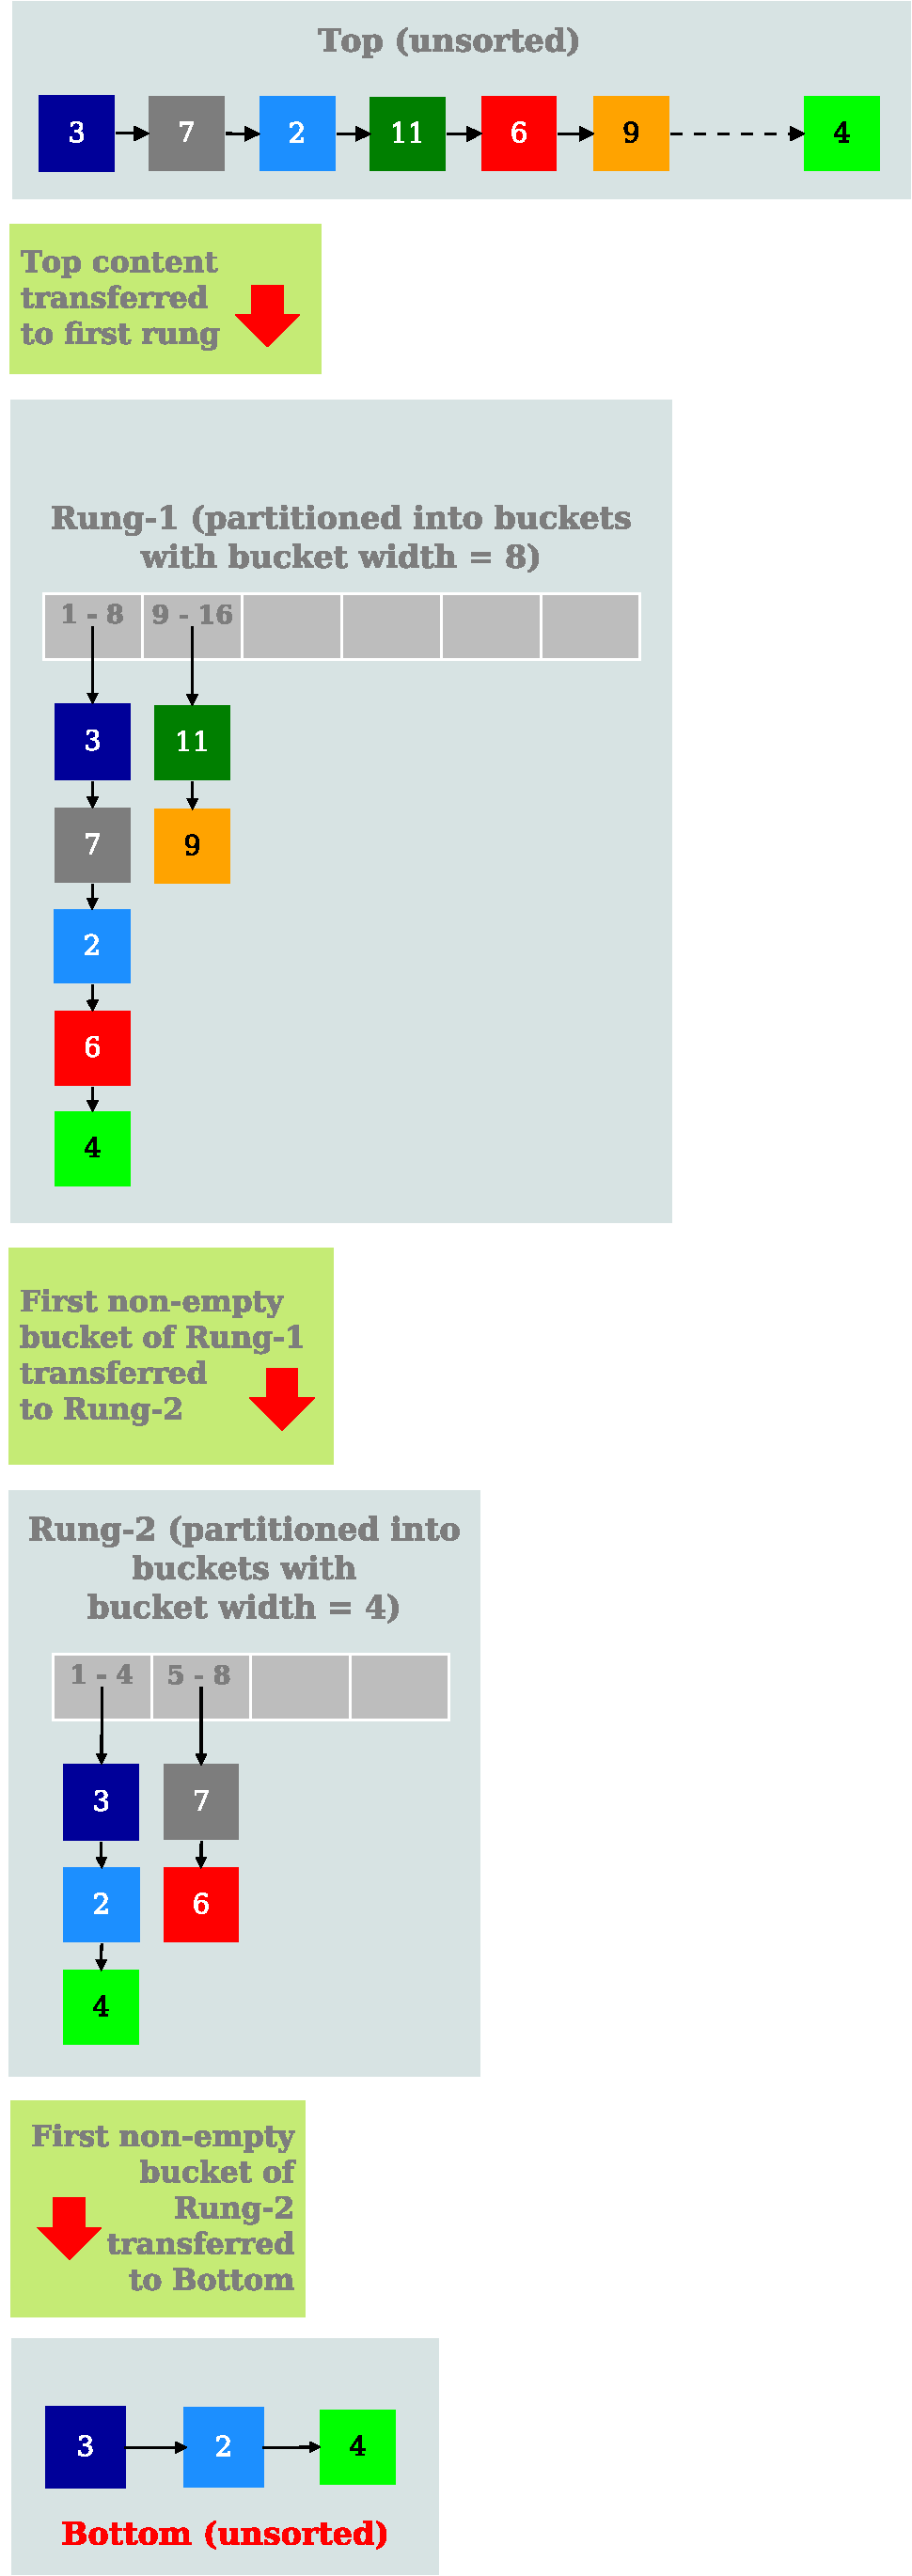
\includegraphics[width=0.39\textwidth]{figures/ladderq_unsorted_bottom}}
    \caption{\textsc{Ladder Queue} with Unsorted Bottom}
    \label{fig:unsorted_bottom}
\end{figure}

Extending the narrative in Section \ref{subsec:ladderq}, the Ladder Queue \cite{tang-05} structure can be
modified for use as a partially sorted priority queue. Since the Ladder Queue efficiently groups events within
a small time interval, Bottom most likely contains events that are causally independent.  Any Time
Warp-synchronized PDES simulator greedily processes events and has the ability to recover from causal
violations (events processed out-of-order in an LP) if detected within a reasonable time interval.  Under
ideal circumstances, events inside Bottom would be causally independent and it should be possible to process
them without the need to sort them based on their timestamp.  Replacing the priority queue in the Bottom
structure with any unsorted container should allow the simulator to process events without incurring frequent
rollbacks and also save valuable time that otherwise would have been wasted on sorting. Even though
\emph{Unsorted Bottom} may not be an effective event scheduling strategy for a wide spectrum of simulation
models, results presented in \cite{gupta-14} indicate that it is suited for Time-Warp compatible models.

Similar to the modifications proposed to the ``insert event'' operation in Section \ref{subsec:ladderq},
Bottom is not split any further when the event count there exceeds a specified threshold.  Separate algorithms
for ``insert'' and ``dequeue'' event are not presented in this section since it is mostly similar to
Algorithms \ref{algo:ladderq_modified_insert} and \ref{algo:ladderq_dequeue} in Section \ref{subsec:ladderq}.

\subsubsection{How to track the minimum event timestamp for GVT calculation?}\label{subsubsec:min_ts_for_gvt}

Section \ref{subsec:global_componenets} gives an overview of the \emph{GVT} estimation algorithm of
\textsc{warped2}.  In order to track the progress made by any individual node, it is necessary to track the
lowest timestamp of events currently present in the \emph{Schedule Queue(s)} on that node.  If the Schedule
Queue is a fully sorted priority queue (such as STL MultiSet, Splay Tree or Ladder Queue), each ``dequeue
event'' operation is sufficient to figure out what is the smallest event present inside the Schedule Queue.
However, for \emph{Ladder Queue with Unsorted Bottom}, the ``dequeue event'' operation is not a reliable
source for reading the lowest timestamp.  This is because the Bottom structure is not sorted.  In order to
track the minimum timestamp, a record is kept of the minimum timestamp whenever a bucket is transferred from
the lowest rung to the Bottom.  This record is updated every time the Bottom runs out of events and another
bucket is transferred to Bottom.  This record is also updated if the ``insert event'' operation inserts an
event into Bottom whose timestamp is smaller than the recorded minimum timestamp.

\subsection{Ladder Queue with Lock-free Unsorted Bottom}\label{subsec:lockfree}

In \textsc{warped2}, locks (Mutex \cite{dijkstra-65} or Ticket Lock \cite{mellor-91}) regulate access to the
shared Schedule Queue(s).  Algorithm \ref{algo:detailed_event_loop} shows that \texttt{lockScheduleQueue()}
and \texttt{unlockScheduleQueue()} are used to regulate access to the Schedule Queue when worker threads try
to access it for dequeuing and inserting events.  This coarse-grained locking strategy works efficiently for
concurrent access to priority queues which do not have any hierarchical internal arrangement.  However, when
hierarchically-structured Ladder Queue with Unsorted Bottom is used as the Schedule Queue, a fine-grained
locking strategy may improve the efficiency of concurrent operations on the queue.  Based on the hypothesis
proposed in Section \ref{subsec:unsorted_bottom} that eliminates the need to sort pending events inside
Bottom, a \emph{Lock-Free Unsorted List} \cite{fomitchev-04,valois-95,harris-01, zhang-13} could serve as
Bottom while the rest of the Ladder Queue (Top and Rungs) is protected by a common lock.

Survey of the literature available on non-blocking and lock-free data structures reveals several options for
lock-free lists and queues \cite{valois-95, michael-95, michael-96, michael-98, michael-02, michael-04,
  fomitchev-04, zhang-13, harris-01}.  Among these choices, a promising option is the \texttt{LFList}, a
lock-free list developed by Zhang \emph{et al} \cite{zhang-13}.  The LFList is easy to adopt into the Ladder
Queue library but it lacks a ``dequeue'' mechanism.  A modified version of the LFList, proposed by Gupta
\emph{et al} \cite{gupta-14}, provides this dequeue functionality and also eliminates features which are
unnecessary for \textsc{warped2}.  The LFList uses backward link (\texttt{prev}) and thread ID (\texttt{tid})
which are relevant for doubly linked lists and for a wait-free queue derivative respectively.  Such features
are an overkill for unsorted Bottom in the Ladder Queue and requires only a singly-linked list to store
unsorted events within a small time window.  Preliminary results presented in \cite{gupta-14} highlights the
potential performance benefits of this approach.

The Ladder Queue (shown in Figures \ref{fig:ladderq_sorted} and \ref{fig:unsorted_bottom}) allows three basic
operations for manipulation of the pending event set, namely:

\begin{enumerate}
\item \emph{Insert} a newly scheduled event from an Input Queue to the Schedule Queue,
\item \emph{Dequeue} a scheduled event from the Schedule Queue for processing, and
\item \emph{Erase} a scheduled event from the Schedule Queue when a straggler or anti-message is detected.
\end{enumerate}

In the default design of \textsc{warped2}, a Schedule Queue lock makes these operations thread-safe for each
Schedule Queue.  As the number of worker threads per Schedule Queue increases, contention for this lock also
increases.  A lock-free list, on the other hand, uses compare-and-swap (CAS) instructions and can scale
significantly better than a lock-protected queue as the number of threads increase.  As mentioned above,
Bottom can be implemented as a lock-free list but a common lock still needs to protect the internal Ladder
structures, namely Top and Rung(s).  This arrangement will allow threads to atomically dequeue from Bottom
while another thread can acquire the lock in parallel and insert an event into Top or Rung(s) and re-organize
the buckets.  The set of Schedule Queue operations needed for a Ladder Queue with Lock-free Unsorted Bottom
can be further simplified as follows:

\begin{enumerate}

\item If a newly scheduled event needs to be \emph{inserted} into the lock-free Bottom, it can be inserted at
  the head of the list using one CAS operation.  Threads will still have to contest for access to the common
  lock if this new event has to be inserted into Top or Rungs instead of Bottom.

\item A scheduled event can be \emph{dequeued} from head of the lock-free Bottom using one CAS operation.  If
  the Bottom is empty, threads will need access to the common lock for pulling events down from Top or Rungs
  into Bottom.  The transfer of events from the chosen rung bucket to Bottom will be done using lock-free
  operations.
    
\item \emph{Erase} is not a necessary operation for Time Warp.  The simulation can rollback to a consistent
  state if a scheduled event is not immediately removed from the Schedule Queue when a straggler or
  anti-message is detected.  The erase operation is a relatively complex operation for lock-free lists and
  this complexity is avoidable for Time Warp-synchronized simulators at the expense of delayed rollbacks of
  longer length.

\end{enumerate}

\subsubsection{Lock-Free List in \textsc{warped2}}\label{subsubsec:lockfree_list}

The Lock-Free List used to create the \emph{Unsorted Bottom} for the Ladder Queue is a simple singly-linked
list.  Each node on this list has two attributes: \texttt{DATA} for storing the event and \texttt{NEXT} for
storing the address of the next node on that list.  The lock-free list only supports ``insert'' and
``dequeue'' operations on the \texttt{HEAD} of the list.  Figures \ref{fig:lockfree_insert} and
\ref{fig:lockfree_dequeue} illustrate these operations. Algorithms \ref{algo:lockfree_insert} and
\ref{algo:lockfree_dequeue} provide further details.

\begin{figure}
    \centering
    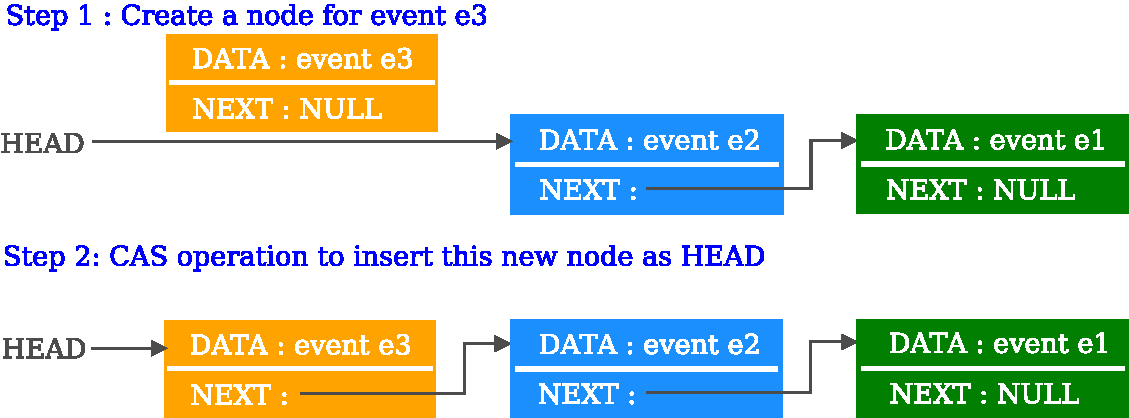
\includegraphics[width=0.7\textwidth]{figures/insert_lockfree.pdf}
    \caption{Insert Operation on Lock-Free List}\label{fig:lockfree_insert}
\end{figure}

\begin{algorithm}
\DontPrintSemicolon
\SetKwFunction{cas}{CAS}
\SetKwFunction{success}{SUCCESS}

    Create a new node $x$\;
    $x\rightarrow$DATA $\gets$ event $e$\;
    \;
    node $m \gets$ HEAD\;
    $x\rightarrow$NEXT $\gets m$\;
    \While{$\cas{\&HEAD, \&m, x} \neq \success$}{
        $m \gets$ HEAD\;
        $x\rightarrow$NEXT $\gets m$\;
    }
    \;
\caption{Lock-Free List Insert Event}\label{algo:lockfree_insert}
\end{algorithm}

\begin{figure}
    \centering
    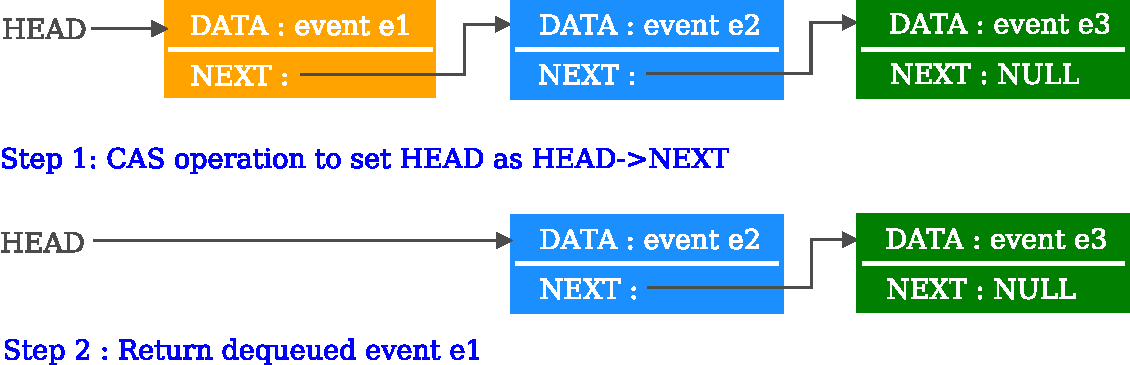
\includegraphics[width=0.7\textwidth]{figures/dequeue_lockfree.pdf}
    \caption{Dequeue Operation on Lock-Free List}\label{fig:lockfree_dequeue}
\end{figure}

\begin{algorithm}
\DontPrintSemicolon
\SetKw{Return}{return}
\SetKwFunction{cas}{CAS}
\SetKwFunction{success}{SUCCESS}

    node $m \gets$ HEAD\;
    \If{$m \in$ NULL}{
        $\Return$ NULL\;
    }
    \;
    \While{$\cas{\&HEAD, \&m, m$\rightarrow$NEXT} \neq \success$}{
        $m \gets$ HEAD\;
        \If{$m \in$ NULL}{
            $\Return$ NULL\;
        }
    }
    \Return $m\rightarrow$DATA\;
    \;
\caption{Lock-Free List Dequeue Event}\label{algo:lockfree_dequeue}
\end{algorithm}

Algorithms \ref{algo:ladderq_lockfree_insert} and \ref{algo:ladderq_lockfree_dequeue} show how the ``insert''
and ``dequeue'' operations will work when a Lock-Free List is used to create a Ladder Queue with Lock-Free
Unsorted Bottom.  The \texttt{lock()} and \texttt{unlock()} functions acquire and release the common lock
respectively and protects access to Top and any available Rungs.

\vspace{0.4in}
\begin{algorithm}
\DontPrintSemicolon
\SetKw{Return}{return}
\SetKwFunction{timestamp}{timestamp}
\SetKwFunction{sizeThreshold}{sizeThreshold}
\SetKwFunction{minTS}{minTS}
\SetKwFunction{bucketWidth}{bucketWidth}
\SetKwFunction{size}{size}
\SetKwFunction{lock}{lock}
\SetKwFunction{unlock}{unlock}

    \lock{}\;
    \If{$e\rightarrow\timestamp{} \geq Top.\minTS$}{
        Insert event $e$ into tail of $Top$\;
        \unlock{}\;
        \Return\;
    }
    \;
    \While{$e\rightarrow\timestamp{} < Rung[x].\minTS$}{
        x++\;
    }
    \;
    \If{$x \in$ valid rung}{
        \;
        bucket $k \gets \frac{e\rightarrow\timestamp{} - Rung[x].\minTS}{Rung[x].\bucketWidth}$\;
        \;
        Insert event $e$ into tail of bucket $k$ of rung $x$\;
        \unlock{}\;
        \Return\;
    }
    \unlock{}\;
    \;
    Insert event $e$ into lock-free $Bottom$\;
    \Return\;
    \;
\caption{\textsc{Ladder Queue} Lock-Free Insert Operation}
\label{algo:ladderq_lockfree_insert}
\end{algorithm}

\begin{algorithm}
\DontPrintSemicolon
\SetKw{Return}{return}
\SetKwFunction{timestamp}{timestamp}
\SetKwFunction{minTS}{minTS}
\SetKwFunction{maxTS}{maxTS}
\SetKwFunction{bucketWidth}{bucketWidth}
\SetKwFunction{size}{size}
\SetKwFunction{lock}{lock}
\SetKwFunction{unlock}{unlock}

    event $e \gets$ dequeue from lock-free $Bottom$\;
    \If{$e \in$ valid event}{
        \Return $e$\;
    }
    \;
    \lock{}\;
    \If{Rung(s) exist}{
        Find first non-empty bucket $k$ in the lowest available rung $x$\;
        Transfer events from bucket $k$ in rung $x$ to $Bottom$\;
        Delete rung $x$ if it has no non-empty buckets left\;
        \unlock{}\;
        \;
        event $e \gets$ dequeue event from lock-free $Bottom$\;
        \Return $e$\;
    }
    \;
    \textit{/* Transfer events from Top into Rung(s) and Bottom */}\;
    \;
    $Rung[1].\bucketWidth \gets \frac{Top.\maxTS - Top.\minTS}{Top.\size}$\;
    \;
    $Rung[1].\minTS \gets Top.\minTS$\;
    Transfer $Top$ into $Rung[1]$\;
    $Top.\minTS \gets Top.\maxTS$\;
    Find first non-empty bucket $k$ in $Rung[1]$\;
    Transfer events from bucket $k$ in $Rung[1]$ to $Bottom$\;
    Delete $Rung[1]$ if it has no non-empty buckets left\;
    \unlock{}\;
    \;
    event $e \gets$ dequeue event from lock-free $Bottom$\;
    \Return $e$\;
    \;
\caption{\textsc{Ladder Queue} Lock-Free Dequeue Operation}
\label{algo:ladderq_lockfree_dequeue}
\end{algorithm}

\section[\textsc{Scheduling Techniques}]{Techniques for Scheduling Pending Events}\label{sec:scheduling_techniques}

The \emph{Pending Event Set} in \textsc{warped2} uses a two-level hierarchical arrangement.  Figure
\ref{fig:timewarp_pending_event_set} illustrates this design and Section \ref{subsec:pending_event_set}
provides detailed explanation for the different different data structures that combine together to form the
\emph{pending event set}.  However, Algorithm \ref{algo:event_loop} only provides a simplistic overview of how
events are processed in \textsc{warped2}.  It does not provide any details about how locks are implemented to
serialize access by multiple threads to the \emph{Input Queue} and \emph{Schedule Queue}.  Algorithm
\ref{algo:detailed_event_loop} presents the missing details which will be needed to continue the discussion in
later sections of this chapter.

\begin{algorithm}
\DontPrintSemicolon
\SetKw{Continue}{continue}
\SetKwFunction{getNextScheduledEvent}{getNextScheduledEvent}
\SetKwFunction{lockScheduleQueue}{lockScheduleQueue}
\SetKwFunction{unlockScheduleQueue}{unlockScheduleQueue}
\SetKwFunction{timestamp}{timestamp}
\SetKwFunction{reportMinTimeForGVT}{reportMinTimeForGVT}
\SetKwFunction{lockInputQueue}{lockInputQueue}
\SetKwFunction{unlockInputQueue}{unlockInputQueue}

    \While{signal to terminate not detected}{
        $\lockScheduleQueue{}$\;
        $e \gets \getNextScheduledEvent{}$\;
        $\unlockScheduleQueue{}$\;
        \;
        $LP \gets$ receiver of $e$\;
        \;
        $\reportMinTimeForGVT(\ thread\_id\ ,\ e\rightarrow\timestamp{}\ )$\;
        \;
        \If{$e <$ last processed event for $LP$}{
            Rollback $LP$\;
        }
        \;
        \If{$e$ is an anti-message}{
            Cancel event with $e$ (if possible)\;
            Schedule new events for $LP$\;
            \Continue\;
        }
        \;
        Process event $e$\;
        Save state of $LP$\;
        Send newly generated events to their destinations\;
        \;
        Call $\lockInputQueue{}$ for the $LP$\;
        \;
        Move $e$ to Processed Queue\;
        \;
        $\lockScheduleQueue{}$\;
        Replace scheduled event for $LP$ with an event from the Input Queue
        (if available)\;
        $\unlockScheduleQueue{}$\;
        \;
        Call $\unlockInputQueue{}$ for the $LP$\;\;
    }

\caption{\textsc{warped2} Event Processing Loop (Detailed)}\label{algo:detailed_event_loop}
\end{algorithm}

As shown in Algorithm \ref{algo:detailed_event_loop}, \texttt{lockInputQueue()} and
\texttt{lockScheduleQueue()} protects access to the Input Queues and the Schedule Queue respectively.  Each
thread reports the timestamp of the event it is currently processing using \texttt{reportMinTimeForGVT()} for
\emph{GVT} estimation.

\subsubsection{\textbf{Should \textsc{warped2} process pending events in \emph{groups} or in
\emph{parallel} instead of one at a time?}}
\label{subsubsec:should_parallelize}

Due to the rapid growth in number of on-chip cores, contention for shared data structures has increased
\cite{ghuloum-09}.  Multiple threads attempt to access the \emph{Pending Event Set} data structures for
scheduling the next event for execution.  Event executions are generally fine-grained in parallel simulation.
This quickly leads to non-trivial contention for the pending event set.  If threads are provided the option to
process events in either groups or in parallel, they will spend less time in waiting for access to these
shared data structures.

Section \ref{subsec:multiple_scheduleq} describes a ``divide-and-conquer'' strategy of partitioning the
\emph{pending event set} into multiple \emph{Schedule Queues} in order to boost parallel processing of pending
events.  Sections \ref{subsec:chains}, \ref{subsec:block_scheduling} and \ref{subsec:bags} proposes techniques
for scheduling pending events in groups.

\subsection{Multiple Schedule Queues}\label{subsec:multiple_scheduleq}

\begin{figure}
    \centering
    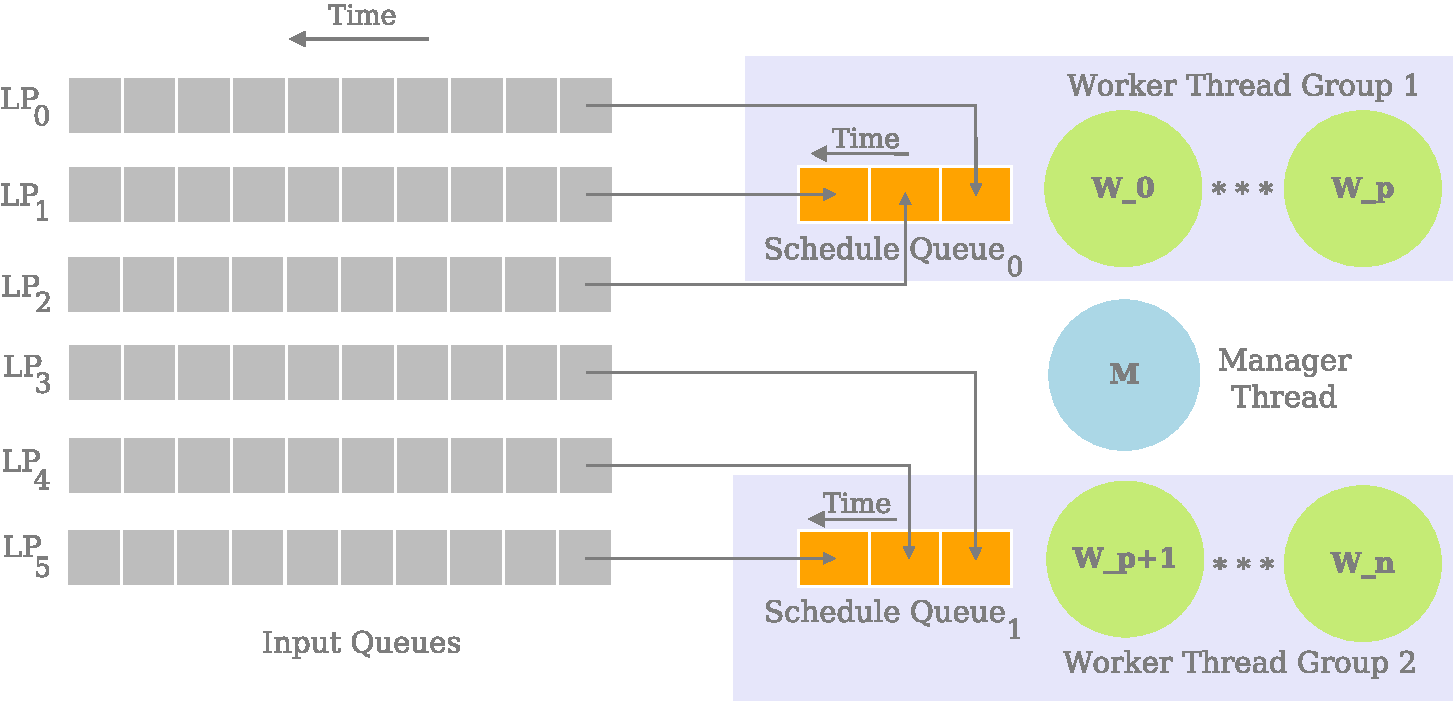
\includegraphics[width=0.95\textwidth]{figures/multiple_scheduleq.pdf}
    \caption{Multiple Schedule Queues in \textsc{warped2}}\label{fig:multiple_scheduleq}
\end{figure}

In order to reduce the contention for common \emph{Schedule Queue} on a multi-core processing platform,
Dickman \emph{et al} \cite{dickman-13} proposed the use of multiple \emph{Schedule Queues} in
\textsc{warped2}.  The \emph{Input Queues} are split into groups where each LP group has its own
\emph{Schedule Queue} and \emph{Schedule Queue Lock}.  The thread pool is also split into groups with each
\emph{Schedule Queue} having access to its own private pool of threads.  Algorithm
\ref{algo:multiple_scheduleq_event_loop} shows how events can be processed using this arrangement.

\begin{algorithm}
\DontPrintSemicolon
\SetKw{Continue}{continue}
\SetKwFunction{getNextScheduledEvent}{getNextScheduledEvent}
\SetKwFunction{lockScheduleQueue}{lockScheduleQueue}
\SetKwFunction{unlockScheduleQueue}{unlockScheduleQueue}
\SetKwFunction{getScheduleQueueId}{getScheduleQueueId}
\SetKwFunction{timestamp}{timestamp}
\SetKwFunction{reportMinTimeForGVT}{reportMinTimeForGVT}
\SetKwFunction{lockInputQueue}{lockInputQueue}
\SetKwFunction{unlockInputQueue}{unlockInputQueue}

    \While{signal to terminate not detected}{
        \;
        $schedule\_queue\_id \gets \getScheduleQueueId(thread\_id)$\;
        $\lockScheduleQueue(schedule\_queue\_id)$\;
        $e \gets \getNextScheduledEvent{schedule\_queue\_id}$\;
        $\unlockScheduleQueue(schedule\_queue\_id)$\;
        \;
        $LP \gets$ receiver of $e$\;
        \;
        $\reportMinTimeForGVT(\ thread\_id\ ,\ e\rightarrow\timestamp{}\ )$\;
        \;
        \If{$e <$ last processed event for $LP$}{
            Rollback $LP$\;
        }
        \;
        \If{$e$ is an anti-message}{
            Cancel event with $e$ (if possible)\;
            Schedule new events for $LP$\;
            \Continue\;
        }
        \;
        Process event $e$\;
        Save state of $LP$\;
        Send newly generated events to their destinations\;
        \;
        Call $\lockInputQueue{}$ for the $LP$\;
        \;
        Move $e$ to Processed Queue\;
        \;
        $\lockScheduleQueue(schedule\_queue\_id)$\;
        Replace scheduled event for $LP$ with an event from the Input Queue
        (if available)\;
        $\unlockScheduleQueue(schedule\_queue\_id)$\;
        \;
        Call $\unlockInputQueue{}$ for the $LP$\;\;
    }

\caption{\textsc{warped2} Event Processing Loop for Multiple Schedule Queues}
\label{algo:multiple_scheduleq_event_loop}
\end{algorithm}

There is a greater risk of events being processed out-of-order in this arrangement.  Multiple \emph{Schedule
  Queues} processing events independently might process events ``too greedily'' and throw the scheduling
mechanism off-balance.  If that happens, the Time Warp mechanism will identify any causal violation and
initiate the recovery process via \emph{rollbacks}.  The motivation behind splitting the common Schedule Queue
is to aim for overall gain in computing time by reducing contention for the \emph{Schedule Queue lock}.
Imbalance, which is a side-effect of this arrangement, may lead to loss of computing time due to extra
rollbacks.  As long as this loss does not override the gains made from reduction in lock contention, this
arrangement would be a promising option on multi-core processing platforms.

\subsection{Chains}\label{subsec:chains}

\subsubsection{Inferences drawn from Quantitative Analysis}\label{subsubsec:inferences}

As evident from the details presented so far in this thesis, one of the the key areas of focus for
\textsc{warped2} is \emph{contention management} in the pending event set.  Chapter
\ref{chapter:event_scheduling} presents the various avenues that have been explored to date.  In addition,
some foundational studies were also conducted in the past few years on partitioning of simulation models
\cite{alt-14} and transactional memory-based access to the pending event set \cite{hay-15}, but with only
limited success.

\begin{figure}
    \centering
    \begin{subfigure}{.48\textwidth}
        \centering
        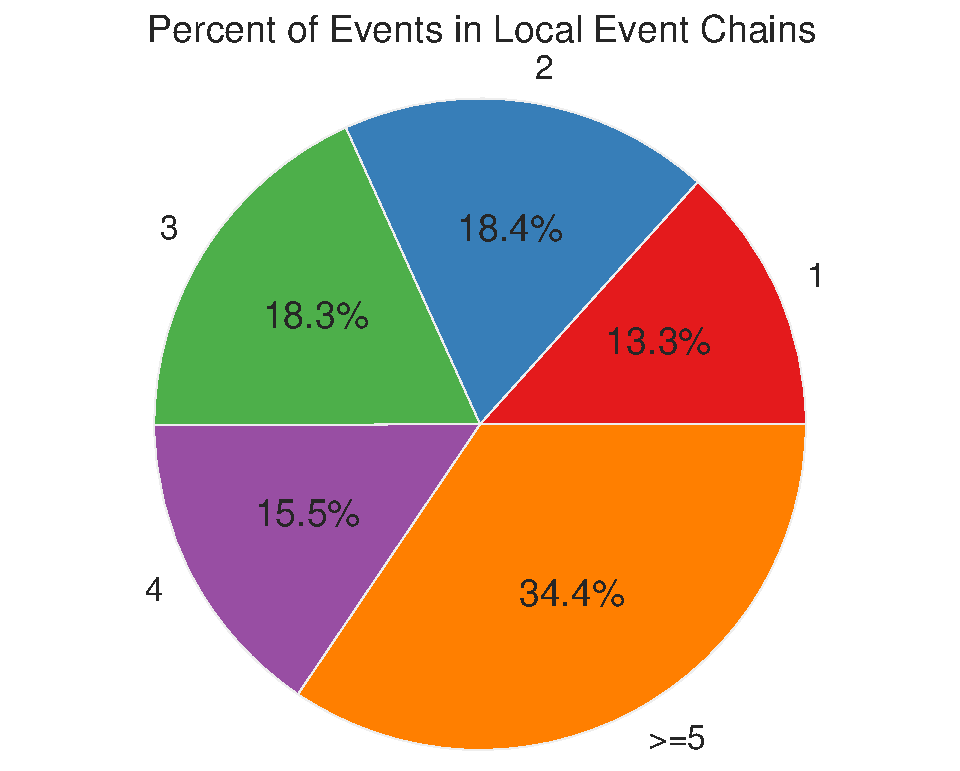
\includegraphics[width=1\textwidth]{figures/local_event_chain/traffic_total.pdf}
    \end{subfigure}
    \begin{subfigure}{.48\textwidth}
        \centering
        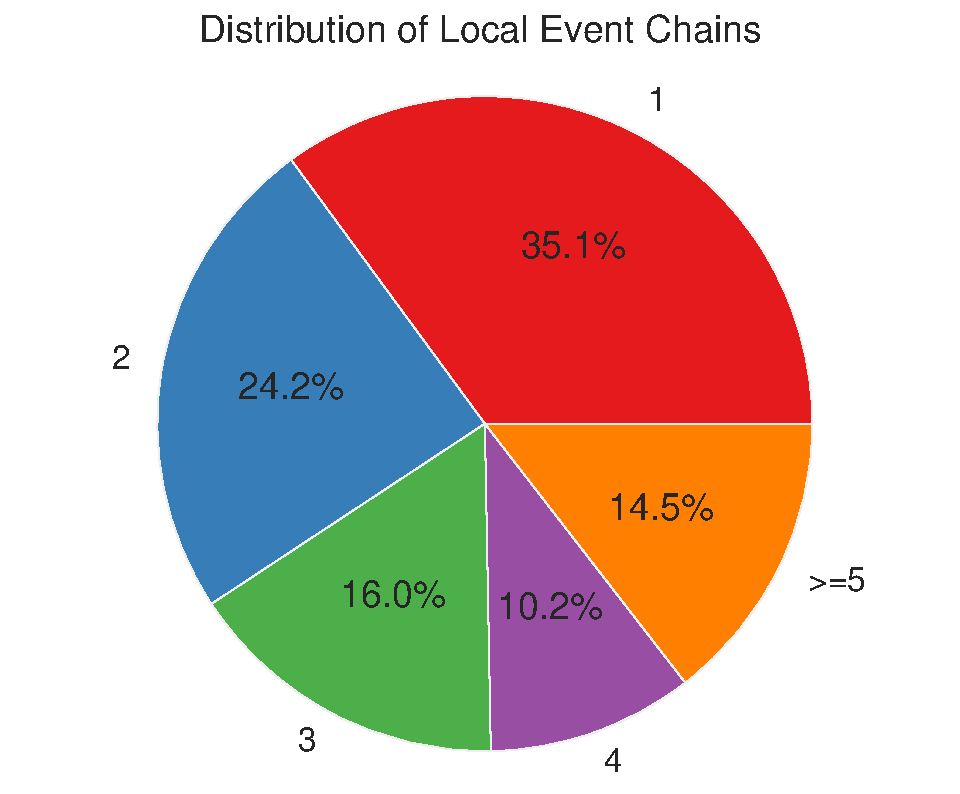
\includegraphics[width=1\textwidth]{figures/local_event_chain/traffic_summary.pdf}
    \end{subfigure}
    \caption{Traffic Model : Local Event Chains}
    \label{fig:local_event_chain:traffic}
\end{figure}

\begin{figure}
    \centering
    \begin{subfigure}{.48\textwidth}
        \centering
        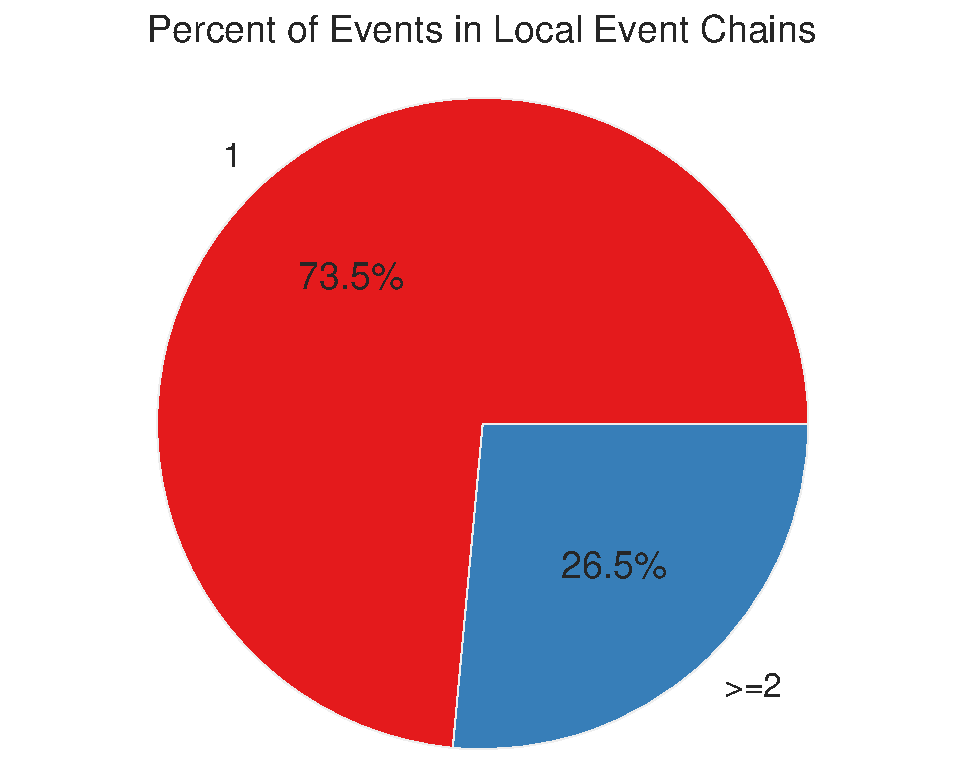
\includegraphics[width=1\textwidth]{figures/local_event_chain/epidemic_total.pdf}
    \end{subfigure}
    \begin{subfigure}{.48\textwidth}
        \centering
        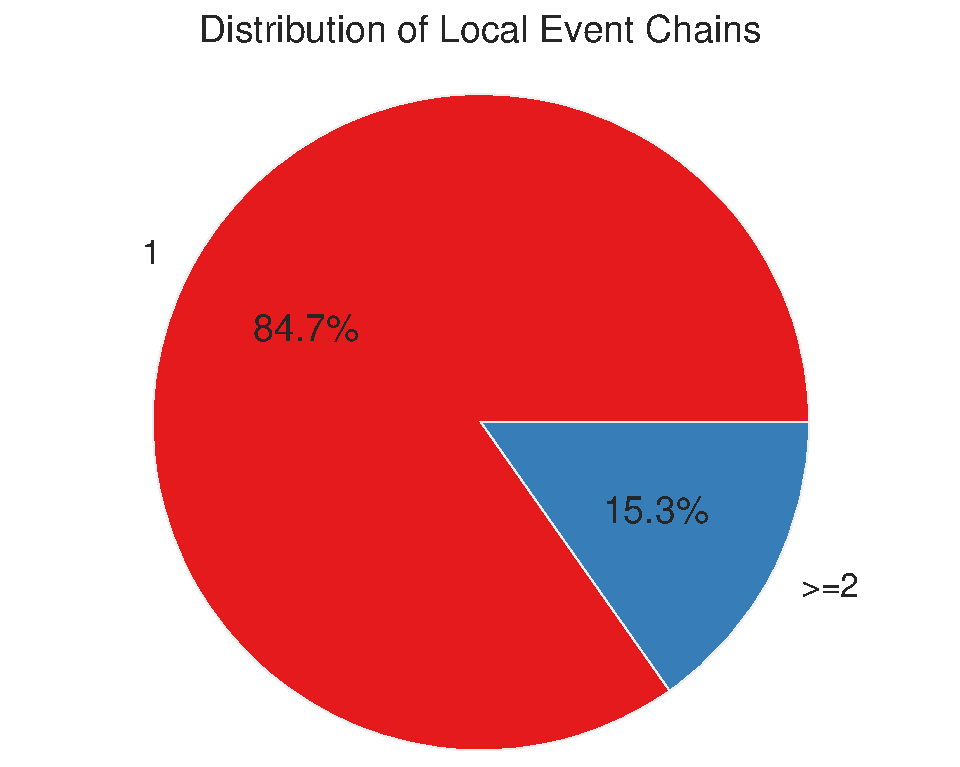
\includegraphics[width=1\textwidth]{figures/local_event_chain/epidemic_summary.pdf}
    \end{subfigure}
    \caption{Epidemic Disease Propagation Model : Local Event Chains}
    \label{fig:local_event_chain:epidemic}
\end{figure}

\begin{figure}
    \centering
    \begin{subfigure}{.48\textwidth}
        \centering
        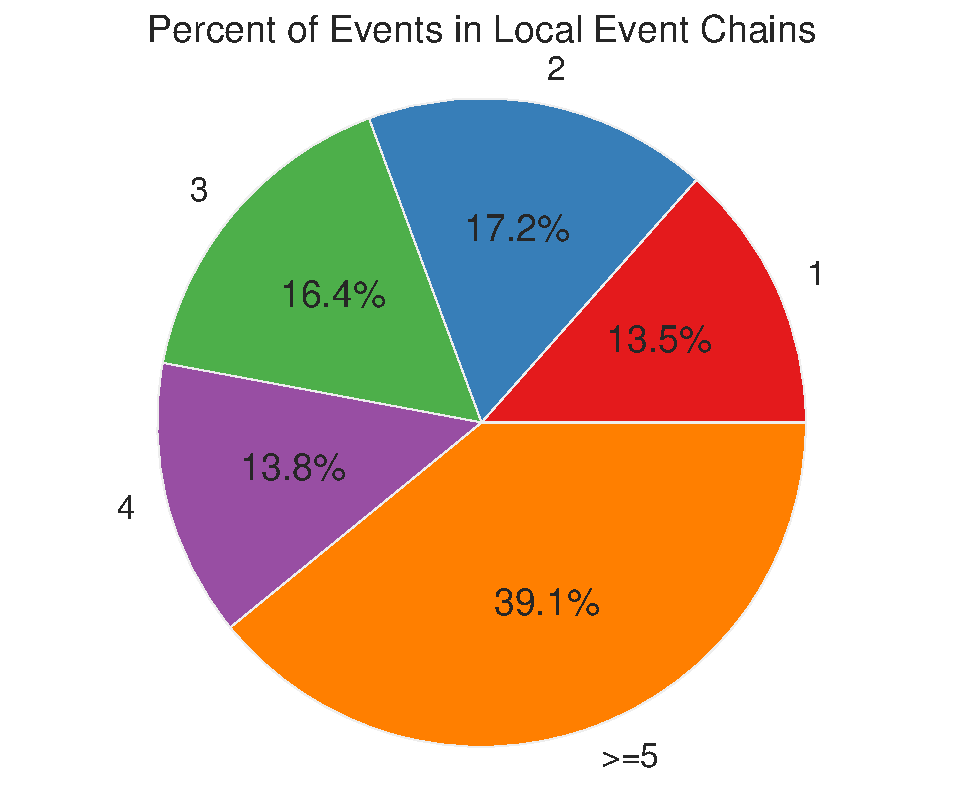
\includegraphics[width=1\textwidth]{figures/local_event_chain/pcs_total.pdf}
    \end{subfigure}
    \begin{subfigure}{.48\textwidth}
        \centering
        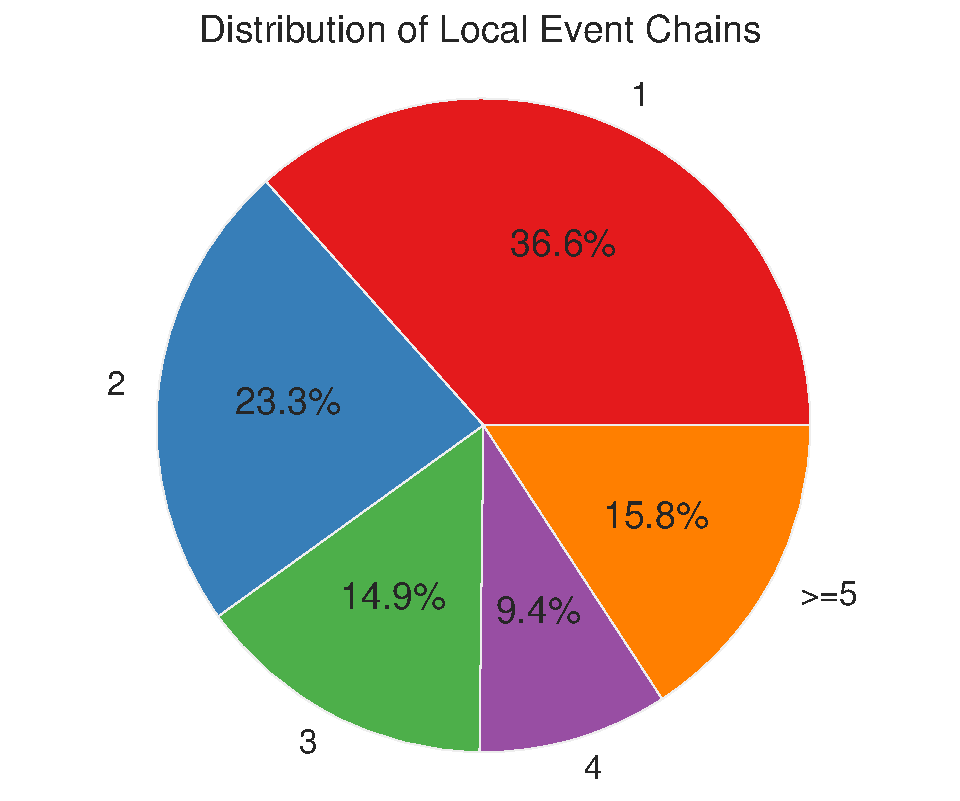
\includegraphics[width=1\textwidth]{figures/local_event_chain/pcs_summary.pdf}
    \end{subfigure}
    \caption{Portable Cellular Service Model : Local Event Chains}
    \label{fig:local_event_chain:pcs}
\end{figure}

Wilsey \cite{wilsey-16} published a quantitative study on the runtime profile of events generated from the
simulation traces of events processed.  A key metric in that study was the \emph{event chain}, which is a
collection of pending events from an LP that could potentially be executed as a group.  The rationale is, at
any point in the simulation, an event chain would contain all events from an LP that are available for
immediate execution in the pending event set.  The event chain of an LP is treated as a single entity and the
scheduling mechanism progresses to the next event once all events in the current chain are processed.  Chains
can be classified into three categories \cite{wilsey-16}, namely: \emph{local}, \emph{linked}, and
\emph{global}.  However, for this discussion, only the local chains are of interest.

If multi-event sized chains are a majority, multiple events can be dequeued for execution by each processing
thread.  Plots on the left side in Figures \ref{fig:local_event_chain:traffic},
\ref{fig:local_event_chain:pcs}, and \ref{fig:local_event_chain:epidemic} show the percentages of total events
in local event chains.  This data is from a previous study \cite{wilsey-16} and it shows that majority of
events in \emph{Portable Cellular Service (PCS)} and \emph{Traffic} models are part of event chains whose
length exceeds 1.  However, only about 27\% of events in \emph{Epidemic} model are part of chains whose length
exceeds 1.  Based on this observation, it would be better from a performance standpoint if pending events from
\emph{PCS} and \emph{Traffic} are scheduled in groups.  For detailed description of the above-mentioned
simulation models, please refer to Section \ref{sec:simulation_models}.

The event chain data also helps us identify chains of variable lengths available at different points during
the simulation.  This helps us quantify the percentages of multi-event scheduling opportunities available.
Plots on the right in Figures \ref{fig:local_event_chain:traffic}, \ref{fig:local_event_chain:epidemic} and
\ref{fig:local_event_chain:pcs} show the fraction of chains of length 1--4 and higher.  If events from
\emph{Traffic} and \emph{PCS} models are scheduled for processing in groups of size $\geq$ 2, the simulator
may have to deal with causality violation 36\% of the time.  The \emph{Epidemic} model has 85\% chance of
suffering causality violations when chain size is $\geq$ 2.

As evident from the discussion above, some models benefit by scheduling events in groups from the pending
event set.  This study presents a conservative snapshot of the event's availability.  Time Warp
synchronization, on the other hand, benefits from the delayed approach to enforcement of causal order.  Thus,
performance of a Time Warp simulation when events are scheduled in groups may exceed what the profile data
suggests.

\subsubsection{Chain Scheduling}\label{subsubsec:chain_scheduling}

\begin{figure}
    \centering
    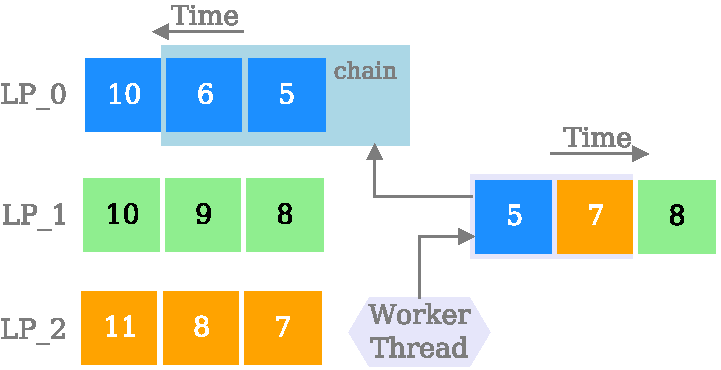
\includegraphics[width=0.6\textwidth]{figures/chain.pdf}
    \caption{\textsc{warped2} Scheduling Technique : Chains}\label{fig:chains}
\end{figure}

\emph{Chain Scheduling} technique is an attempt to understand the extent of parallelism available when a set
of smallest available events from a LP are scheduled for processing.  The goal is to schedule this set (or
\emph{chain}) of events without adversely hampering the performance of \textsc{warped2} due to too many causal
violations.  Each ``dequeue event'' request will remove multiple events from the LP's \emph{Input Queue} along
with the event at the head of the \emph{Schedule Queue}.  These dequeued events are then processed in serial
order.

It would be too optimistic to expect there will not be any causal violations when a chain of events is
processed.  However, Time Warp is a ``checkpointing-and-rollback'' based mechanism that can detect and rectify
itself when it detects causal violations.  This extra workload will add some delay to the overall computing
time.  On the other hand, ``dequeuing'' a set of events from the \emph{Input Queue} saves valuable computing
time that would otherwise be wasted on the wait to acquire the \emph{Schedule Queue Lock} had all events been
scheduled via the \emph{Schedule Queue}.  Thus, \emph{Chain Scheduling} is a compromised design choice which
can out-perform \textsc{warped2}'s default scheduling mechanism (discussed in Section
\ref{subsec:event_processing}) if the computing time saved by reduced lock contention exceeds the time lost
due to extra rollbacks.

There are two approaches for how the output events, generated as a result of this processing, can be
inserted back into the simulation as pending events. These are:

\begin{itemize}

\item Wait till all events from the chain have been processed and then all the output events are inserted back
  into the simulation in bulk.  This approach allows for efficient contention management since worker threads
  will not need to acquire locks inside pending event set frequently.  However, any causal violation (due to
  delay in insertion of output events) will not be detected till at a later time.  This could result in
  \emph{rollbacks} of longer duration.  While testing, this approach proved to be hugely inefficient compared
  to the approach discussed next.  Therefore, \textsc{warped2} does not currently support bulk sending of
  stored output events.  A detailed study is available in \cite{gupta-17}.

\item Insert the output events into the simulation as soon as they are generated.  This approach will increase
  the contention overhead in the shared data structures of the pending event set but will allow the simulator
  to detect causality violations quicker than the the former approach.  A detailed study is available in
  \cite{gupta-17}.

\end{itemize}

After all the ``dequeued events'' in a chain have been processed, the \emph{Schedule Queue} is replenished
with the smallest available unprocessed event from the LP whose events were present in that chain.  The
configurable parameter \emph{chain size} is vital for adjusting the sliding time window within which events
are processed in bulk.  Thus, \emph{chain size} impacts the performance of \textsc{warped2} by affecting the
frequency of rollbacks.

Algorithm \ref{algo:chain_scheduling} shows how chains are scheduled in \textsc{warped2}.  The smallest
available event from the \emph{Schedule Queue} is dequeued using \texttt{getNextScheduledEvent()} and then the
$n$ smallest available events from the corresponding \emph{Input Queue} are read to form the
\emph{chain}.  Another interesting point to note here is that each thread uses \texttt{reportMinTimeForGVT()}
to report the smallest event timestamp for \emph{GVT} calculation.  Normally this would be a simple operation
when scheduling only one event at a time for processing, but here only the timestamp of the smallest event in
the chain is reported.  In this case it happens to be the first event stored inside the \texttt{event\_chain}.

\begin{algorithm}
\DontPrintSemicolon
\SetKw{Continue}{continue}
\SetKw{Break}{break}
\SetKwFunction{getNextScheduledEvent}{getNextScheduledEvent}
\SetKwFunction{lockScheduleQueue}{lockScheduleQueue}
\SetKwFunction{unlockScheduleQueue}{unlockScheduleQueue}
\SetKwFunction{getScheduleQueueId}{getScheduleQueueId}
\SetKwFunction{timestamp}{timestamp}
\SetKwFunction{reportMinTimeForGVT}{reportMinTimeForGVT}
\SetKwFunction{lockInputQueue}{lockInputQueue}
\SetKwFunction{unlockInputQueue}{unlockInputQueue}

    \While{signal to terminate not detected}{
        \;
        $schedule\_queue\_id \gets \getScheduleQueueId(thread\_id)$\;
        $\lockScheduleQueue(schedule\_queue\_id)$\;
        $e \gets \getNextScheduledEvent{schedule\_queue\_id}$\;
        $\unlockScheduleQueue(schedule\_queue\_id)$\;
        \;
        $LP \gets$ receiver of $e$\;
        $LP\rightarrow\lockInputQueue{}$\;
        $event\_chain \gets$ read $n$ events from the Input Queue\;
        $LP\rightarrow\unlockInputQueue{}$\;

        $\reportMinTimeForGVT(\ thread\_id\ ,\ event\_chain[0]\rightarrow\timestamp{}\ )$\;
        \;
        \While{$event\ e \in event\_chain$}{
        
            \If{$e <$ last processed event for $LP$}{
                Rollback $LP$\;
                \Break\;
            }
            \;
            \If{$e$ is an anti-message}{
                Cancel event with $e$ (if possible)\;
                \Continue\;
            }
            \;
            Process event $e$\;
            Save state of $LP$\;
            Send newly generated events to their destinations\;\;
        }
        \;
        Call $\lockInputQueue{}$ for the $LP$\;\;
        Move processed events to Processed Queue\;
        \;
        $\lockScheduleQueue(schedule\_queue\_id)$\;
        Replace scheduled event for $LP$ with an event from the Input Queue
        (if available)\;
        $\unlockScheduleQueue(schedule\_queue\_id)$\;
        \;
        Call $\unlockInputQueue{}$ for the $LP$\;\;
    }

\caption{\textsc{warped2} Event Processing Loop for Chain Scheduling}
\label{algo:chain_scheduling}
\end{algorithm}

\subsection{Block Scheduling}\label{subsec:block_scheduling}

\begin{figure}
    \centering
    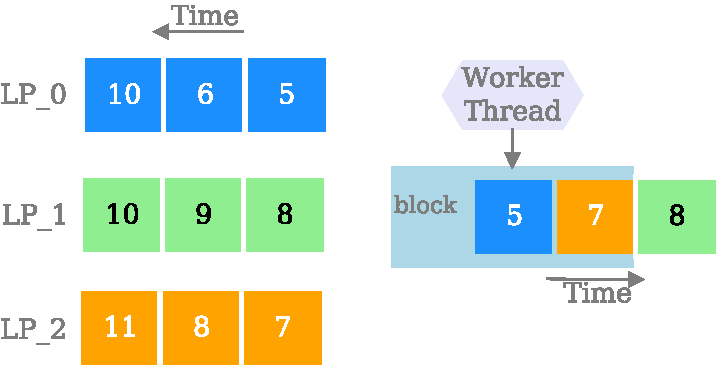
\includegraphics[width=0.6\textwidth]{figures/block.pdf}
    \caption{\textsc{warped2} Scheduling Technique : Blocks}\label{fig:blocks}
\end{figure}

The \emph{Block Scheduling} technique is an attempt to understand the extent of parallelism available when a
set of smallest available pending events from the \emph{Schedule Queue} are scheduled for processing.  The
goal is to process this set (or \emph{block}) of events in serial order without adversely hampering the
performance of \textsc{warped2} due to too many causal violations.  No two events in this \emph{block} belong
to the same LP.

It would be too optimistic to expect there will not be any causal violations when a block of events is
processed.  Fortunately, the Time Warp is a ``checkpointing-and-rollback'' based mechanism that can detect and
rectify itself when it detects causal violations.  This extra workload will add some delay to the overall
computing time.  On the other hand, ``dequeuing'' a set of events from the \emph{Schedule Queue} saves
valuable computing time that would otherwise be wasted on the wait to acquire the \emph{Schedule Queue Lock}
for every scheduled event.  Thus, \emph{Block Scheduling} is a compromised design choice which can out-perform
\textsc{warped2}'s default scheduling mechanism (discussed in Section \ref{subsec:event_processing}) if the
computing time saved by reduced lock contention exceeds the time lost due to extra rollbacks.

In block scheduling, each ``dequeue event'' request will remove multiple events from the \emph{Schedule
  Queue}.  These dequeued events are then processed sequentially. There are two approaches as to how the
output events, generated as a result of this processing, can be inserted back into the simulation as pending
events.  These are:

\begin{itemize}

\item Wait till all events from the block have been processed and then all the output events are inserted back
  into the simulation in bulk.  This approach allows for efficient contention management since worker threads
  will not need to acquire locks inside pending event set frequently.  However, any causal violation (due to
  delay in insertion of output events) will not be detected till at a later time.  This could result in
  \emph{rollbacks} of longer duration.  While testing, this approach proved to be hugely inefficient compared
  to the approach discussed next.  Thus, \textsc{warped2} does not currently support bulk sending of stored
  output events.  A detailed study is available in \cite{gupta-17}.

\item Insert the output events into the simulation as soon as they are generated.  This approach will increase
  the contention overhead in the shared data structures of the pending event set but will allow the simulator
  to detect causality violations quicker than the the former approach.  A detailed study is available in
  \cite{gupta-17}.

\end{itemize}

After all the ``dequeued events'' in a block have been processed, the \emph{Schedule Queue} is replenished
with the smallest available unprocessed event from each of the LPs whose events were present in that block.
Bulk replenishment of the \emph{Schedule Queue} after processing a \emph{block} of events would help reduce
time wasted on contention management in the pending event set.  Similar to \emph{chain size}, the configurable
parameter \emph{block size} is vital for adjusting the sliding time window within which events are processed
in bulk.  That is, \emph{block size} impacts the performance of \textsc{warped2} by affecting the frequency of
rollbacks.

Algorithm \ref{algo:block_scheduling} shows how blocks are scheduled in \textsc{warped2}.  The
\texttt{getNextEventBlock()} dequeues $n$ smallest available events from the \emph{Schedule Queue}.  Each
thread reports the smallest event timestamp for \emph{GVT} calculation using \texttt{reportMinTimeForGVT()}.
Normally this would be a simple operation when scheduling only one event at a time for processing, but here
only the timestamp of the smallest event in the block is reported.  In this case, it happens to be the first
event stored inside the \texttt{event\_block}.

\begin{algorithm}
\DontPrintSemicolon
\SetKw{Continue}{continue}
\SetKwFunction{getNextEventBlock}{getNextEventBlock}
\SetKwFunction{lockScheduleQueue}{lockScheduleQueue}
\SetKwFunction{unlockScheduleQueue}{unlockScheduleQueue}
\SetKwFunction{getScheduleQueueId}{getScheduleQueueId}
\SetKwFunction{timestamp}{timestamp}
\SetKwFunction{reportMinTimeForGVT}{reportMinTimeForGVT}
\SetKwFunction{lockInputQueue}{lockInputQueue}
\SetKwFunction{unlockInputQueue}{unlockInputQueue}

    \While{signal to terminate not detected}{
        \;
        $schedule\_queue\_id \gets \getScheduleQueueId(thread\_id)$\;
        $\lockScheduleQueue(schedule\_queue\_id)$\;
        $event\_block \gets \getNextEventBlock{schedule\_queue\_id}$\;
        $\unlockScheduleQueue(schedule\_queue\_id)$\;
        \;
        $\reportMinTimeForGVT(\ thread\_id\ ,\ event\_block[0]\rightarrow\timestamp{}\ )$\;
        \;
        Create an empty $LP\_list$\;
        \While{$event\ e \in event\_block$}{
            $LP \gets$ receiver of $e$\;
            Insert $LP$ into $LP\_list$\;
            \;
            \If{$e <$ last processed event for $LP$}{
                Rollback $LP$\;
            }
            \;
            \If{$e$ is an anti-message}{
                Cancel event with $e$ (if possible)\;
                \Continue\;
            }
            \;
            Process event $e$\;
            Save state of $LP$\;
            Send newly generated events to their destinations\;\;
        }
        \;
        \For{$ LP \in LP\_list\ $}{
            Call $\lockInputQueue{}$ for the $LP$\;
        }
        \;
        $\lockScheduleQueue(schedule\_queue\_id)$\;
        \For{$ LP \in LP\_list\ $}{
            Move $e$ to Processed Queue\;
            Replace scheduled event for $LP$ with an event from the Input Queue
            (if available)\;
        }
        $\unlockScheduleQueue(schedule\_queue\_id)$\;
        \;
        \For{$ LP \in LP\_list\ $}{
            Call $\unlockInputQueue{}$ for the $LP$\;
        }
        \;
    }

\caption{\textsc{warped2} Event Processing Loop for Block Scheduling}
\label{algo:block_scheduling}
\end{algorithm}

\subsection{Bags}\label{subsec:bags}

\subsubsection{Why are bags an interesting option for scheduling pending events?}\label{subsubsec:why_bag}

Extending the theme set by chain and block scheduling techniques, contention management is the key motivating
factor for organizing pending events into bags.  The goal of this design is to enable threads to process
events from different bags in parallel without long waits for access to the shared data structures.  This
design relies on the hypothesis that pending events grouped into profile-driven partitions will mostly retain
causal order even when these event partitions are processed in parallel.  Thus, in theory, processing bags in
parallel combines the best of both worlds: low contention for shared resources and minimal performance
trade-off due to marginal increase in rollbacks.

\subsubsection{The Louvain Partitioner}\label{subsubsec:louvain}

The \emph{Louvain} method \cite{blondel-08} is a greedy optimization method that can partition large weighted
networks into communities.  Its output is a dendogram that captures the hierarchies of communities.

\emph{Modularity} \cite{newman-06} is a metric used to quantify how effectively the network was partitioned
into different communities (or clusters).  Its value ranges between \emph{-1} and \emph{1} and is a measure of
edge density inside communities compared to edges outside communities.  A high modularity index indicates
dense intra-community nodal connections along with sparse inter-community nodal connections.

Though optimization should in theory yield the best possible solution, it is impractical due to the sheer
volume of cluster combinations possible.  As a result, the \emph{Louvain} method uses a 2-step heuristic
approach to iteratively optimize the \emph{modularity} of partitions:

\begin{enumerate}
\item search for ``small'' communities through local optimization of modularity, and 
\item group together nodes belonging to the same community and construct a secondary network between
  communities.
\end{enumerate}

\begin{figure}
    \centering
    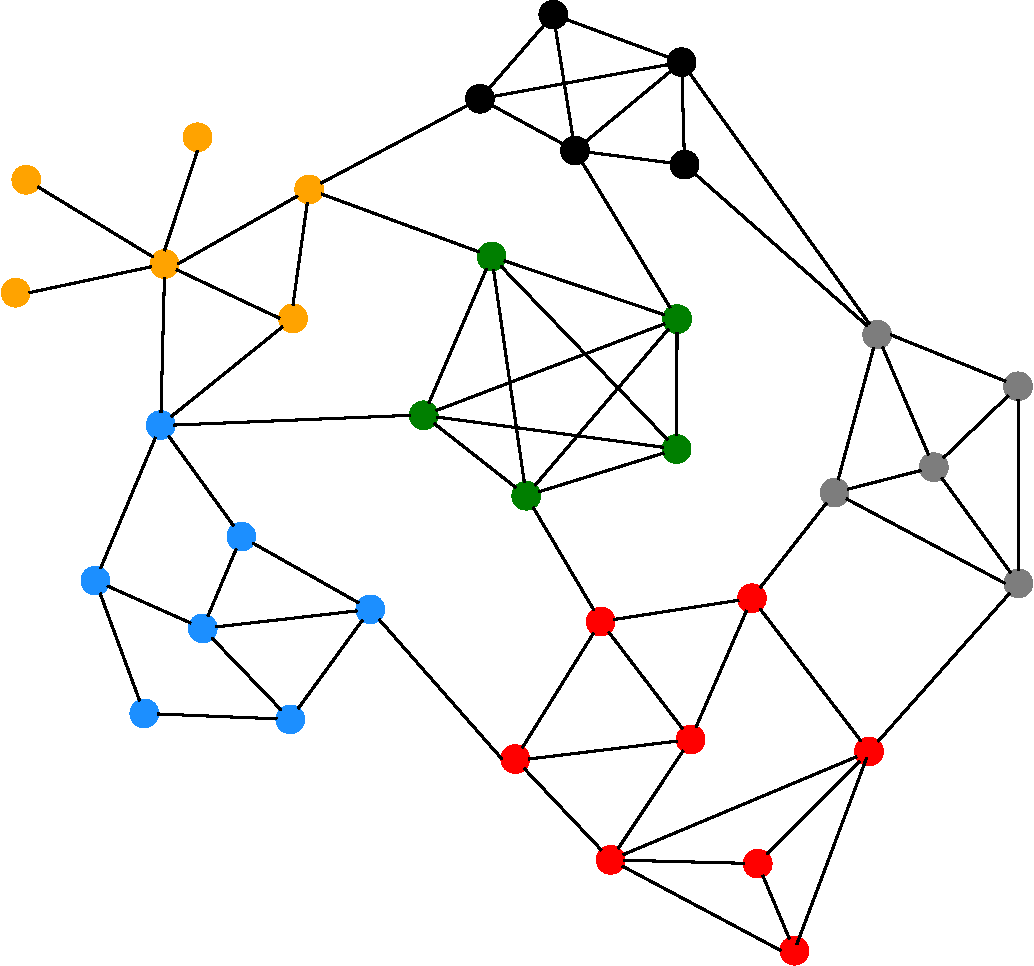
\includegraphics[width=0.4\textwidth]{figures/louvain.pdf}
    \caption{Louvain-based Partitions (shown in different colors)}
    \label{fig:louvain_partitioning}
\end{figure}

Accurate modularity optimization is considered to be a \emph{NP-hard} problem.  However, estimates suggest
that the \emph{Louvain} method has \emph{O(n log n)} amortized time complexity \cite{blondel-08}.  Figure
\ref{fig:louvain_partitioning} illustrates a network partitioned into different communities (each color
indicates a different community).

Crawford \emph{et al} \cite{crawford-17} analyzed the distribution of communities in a simulation of epidemic
disease propagation for \emph{10,000} LPs (refer to Section \ref{subsec:epidemic} for details regarding the
Epidemic model).  They found \emph{54} communities whose LP counts were distributed in the range \emph{50-425}
with the mean at approximately \emph{190}.  Figure \ref{fig:communities} shows this distribution of
communities.

\begin{figure}
    \centering
    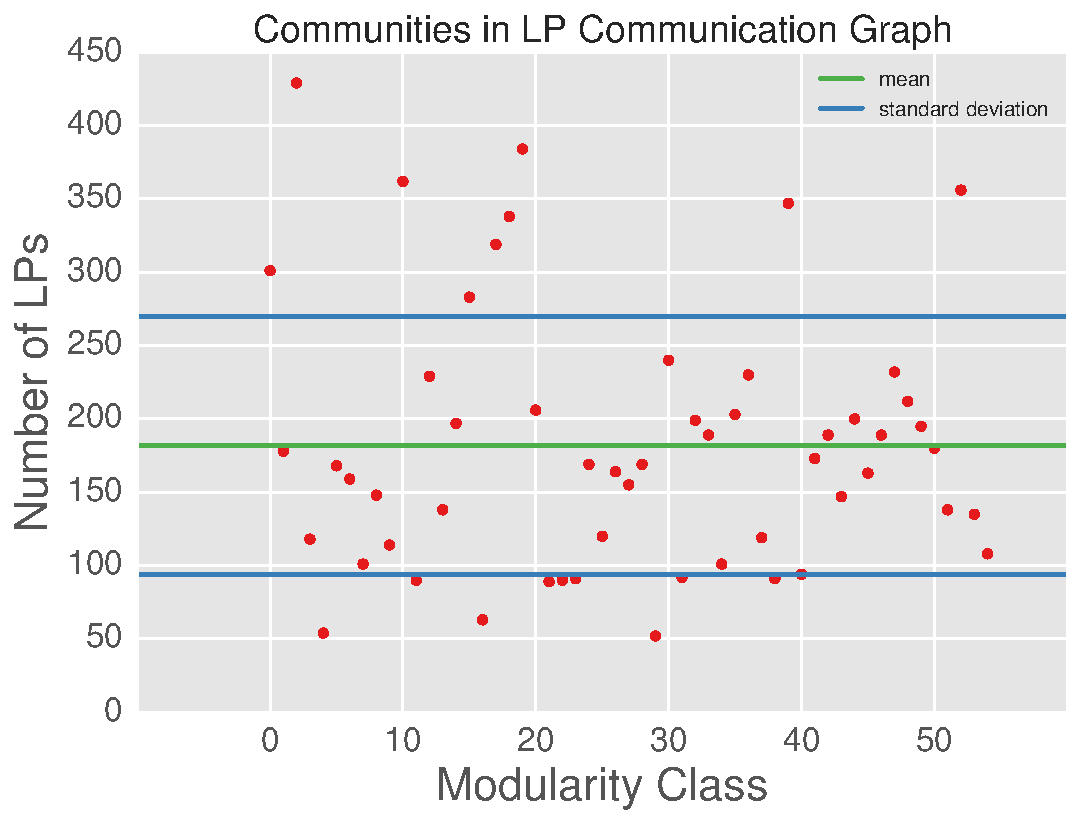
\includegraphics[width=0.7\textwidth]{figures/communities.pdf}
    \caption{Distribution of Communities in `epidemic-10k-ws' model (refer to Table
        \ref{table:epidemic_configs} for model specifications)}
    \label{fig:communities}
\end{figure}

\subsubsection{Organizing Partitions into Bags}\label{subsubsec:bag_organization}

From the perspective of \emph{Discrete Event Simulation}, let us assume that each node in Figure
\ref{fig:louvain_partitioning} represents a Logical Process (LP).  The weight of any edge in the network
equals number of events exchanged between the two LPs connected by that edge.  A network partition (or
community) with high modularity index ideally has dense connections between LPs inside a partition and sparse
connections to LPs outside the partition.  The hypothesis is that densely connected LPs are more likely to
generate events which are \emph{causally linked} than events generated by LPs which are sparesly connected.
Based on this assumption, the LPs from each community can be grouped together to form a \emph{bag} for that
community.  Figure \ref{fig:bag_scheduling} presents a static \emph{Circular Array} whose each element points
to a bag of LPs.  The color and size of each \emph{bag} in Figure \ref{fig:bag_scheduling} matches those of
the corresponding \emph{community} in Figure \ref{fig:louvain_partitioning}.

\begin{figure}
    \centering
    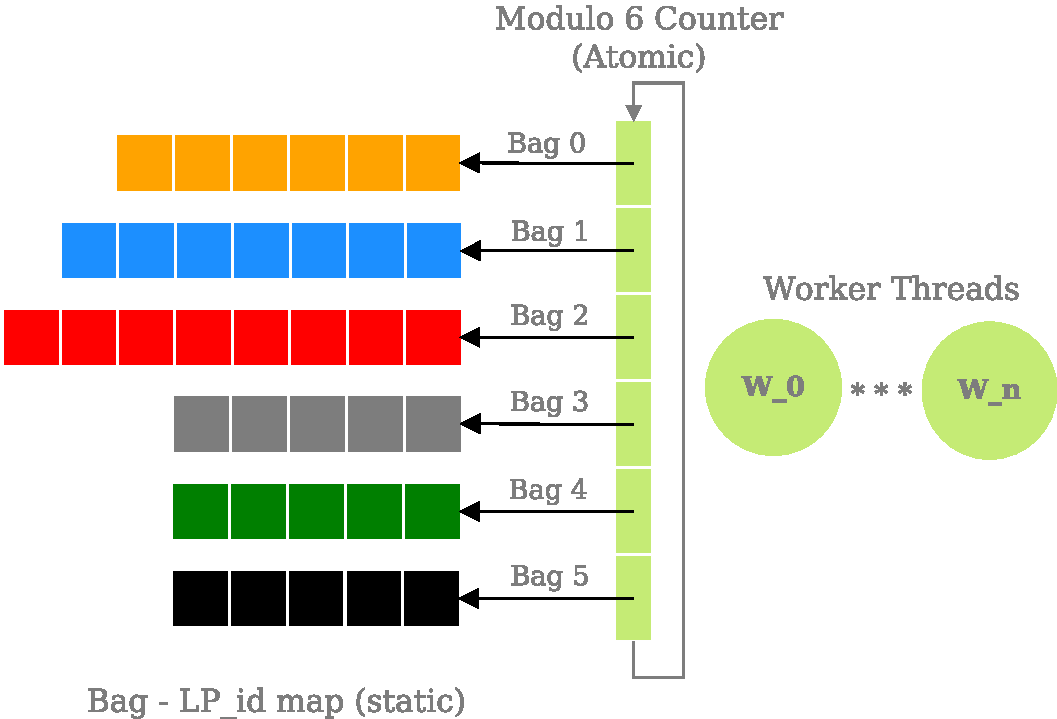
\includegraphics[width=0.75\textwidth]{figures/bags.pdf}
    \caption{\textsc{warped2} Scheduling Technique : Bags}\label{fig:bag_scheduling}
\end{figure}

Each worker thread requests the \emph{modulo N atomic counter} for access to the next available bag in the
circular array.  The size of the static circular array (also called \emph{carousel}) equals the number of bags
(\emph{N}).  Once the thread gets access to a bag, it locks access to that bag and copies the smallest
available unprocessed event from the \emph{Input Queue} of each LP mapped to that bag into an \emph{array}.
It then schedules a part or whole of this unsorted array for processing.  There are three potential benefits
to organizing LPs in the aforementioned way:

\begin{enumerate}

\item The LPs in one bag generally share sparse connections to LPs in other bags.  Assuming this sparse
  connection means events in one bag are more likely to be causally independent of events in other bags over a
  large time window, different threads should be able to process events from different bags in parallel
  without a drastic increase in rollbacks.  The \emph{modulo N counter}, built using \emph{CAS} atomic
  operation, can allow a thread to access a bag from the carousel without the need for any central lock.

\item Dense connections between LPs inside a bag may signify that some or all events in the above-mentioned
  \emph{array} are causally linked.  However, as discussed in Section \ref{subsec:unsorted_bottom}, it is
  reasonable to assume that events within a relatively small time window are causally independent of each
  other.  Therefore, instead of processing all events from the \emph{array}, a worker thread can only process
  those events whose timestamps are within a specified time window.  Much like the \emph{Unsorted Bottom} in
  the Ladder Queue, the events within this time window are not sorted before being processed.  During every
  event processing cycle in \textsc{warped2}, the worker thread calculates the time window's lower and upper
  bounds using one of the following two configurable parameters: T
  \begin{itemize}
  \item \emph{Window Size ($TS_{window}$)} :
    \begin{equation}
      \begin{multlined}
        \interval{\ TS_{min}\ }{\ TS_{min} + TS_{window}\ }, ~~ \text{where}\\
        TS_{min} = \text{timestamp of smallest event in the array.}
      \end{multlined}
      \label{eq:bag_window}
    \end{equation}
    
  \item \emph{Fraction of Bag's Total Window Size ($frac_{\textsc{bag}}$)} :
    \begin{equation}
      \begin{multlined}
        \interval{\ TS_{min}\ }{\ TS_{min} + (TS_{max} - TS_{min}) \times
          frac_{\textsc{bag}}\ }, ~~ \text{where}\\
        TS_{min} = \text{timestamp of smallest event in the array , and}\\
        TS_{max} = \text{timestamp of largest event in the array.}
      \end{multlined}
      \label{eq:bag_fraction}
    \end{equation}
  \end{itemize}
  
\item The carousel and the bags linked to it are static structures.  This means there is no loss of
  performance due to memory allocation and deallocation after initialization.  Even the \emph{array} used to
  temporarily copy the smallest unprocessed events for the bag can be reused for processing the next bag.  This
  drastically reduces the fluctuations in memory usage and boosts performance through reduced need for memory
  I/O.

\end{enumerate}

After the worker thread finishes processing all events scheduled from a bag, it moves these events from the
\emph{Input Queue} to the \emph{Processed Queue} of the corresponding LPs.  It unlocks the bag it was
currently processing and request the atomic counter for the next available bag in the carousel.  It is worth
noting here that the lock for a bag is an atomic flag that is used to prevent multiple worker threads from
accessing a particular bag at the same time.  It is unlikely that there is any significant contention for this
flag because the modulo counter ensures serialized allocation of bags to waiting threads.  Even if a thread is
forced to wait while another thread finishes processing events from a bag, this wait is unlikely to be long
since the thread currently holding the lock is processing events for the previous cycle, but was delayed due
to some reason.

\subsubsection{Distributed Tracking of Simulation's Progress}\label{subsubsec:distributed_time}

The distributed organization of bags complicates how worker threads can asynchronously report the smallest
event timestamp for calculation of the \emph{GVT}.  As mentioned in Section \ref{subsec:global_componenets},
worker threads in \textsc{warped2} work for a process and regularly report the lowest timestamp for that
process.  A worker thread learns the smallest timestamp among events in a bag when it acquires access to that
bag.  A \emph{GVT cycle} for bags is considered complete when worker threads have processed events from all
bags in the carousel in that cycle.  Depending on the speed at which events are processed, a worker thread may
process multiple bags during any GVT cycle but it only reports the smallest timestamp among all events it
processed during that cycle.  During an ongoing GVT cycle, the worker thread reports its minimum timestamp as
the one recorded in the \emph{previous} GVT cycle.

In order to keep track of the minimum timestamp among events processed during any ongoing GVT cycle while also
retaining the minimum timestamp recorded in the previous cycle, each worker thread uses a data structure
called \texttt{minTS\_record} with the following attributes:

\begin{itemize}

\item Current GVT Cycle Count (\texttt{curr\_cycle\_count})
\item Minimum Timestamp recorded during the previous GVT cycle (\texttt{minTS\_prev})
\item Minimum Timestamp recorded during the ongoing GVT cycle (\texttt{minTS\_curr})

\end{itemize}

Algorithm \ref{algo:bags_event_loop} presents how events are processed in bags.  Some of the event set
functions used here have been explained below:

\begin{itemize}

\item \texttt{lockInputQueue()} and \texttt{unlockInputQueue()} controls access to the Input Queues.

\item \texttt{getBag()} fetches the next available bag from the carousel and locks it.  It also increments the
  modulo N atomic counter using Compare-and-Swap (CAS) operation.  If the \texttt{curr\_cycle\_count} is
  smaller than the current GVT cycle count, the worker thread realizes it has entered a new GVT cycle.  In
  that case, it transfers \texttt{minTS\_curr} to \texttt{minTS\_prev} and updates \texttt{curr\_cycle\_count}
  to the current GVT cycle count.

\item \texttt{releaseBag()} releases the lock a worker thread acquired on a bag before processing events from
  that bag.

\item \texttt{fetchLPs()} fetches the list of LPs from the static \emph{carousel} for a particular bag.

\item \texttt{getEvent()} find the smallest available event from the Input Queue of an LP.  The worker thread
  compares this event's timestamp to \texttt{minTS\_curr} and updates the latter if the event's timestamp is
  smaller.

\item \texttt{reportMinTimeForGVT()} is used by each thread to report the smallest timestamp for GVT
  calculation.

\end{itemize}

\begin{algorithm}
\DontPrintSemicolon
\SetKw{Continue}{continue}
\SetKwFunction{lockInputQueue}{lockInputQueue}
\SetKwFunction{unlockInputQueue}{unlockInputQueue}
\SetKwFunction{getBag}{getBag}
\SetKwFunction{releaseBag}{releaseBag}
\SetKwFunction{getEvent}{getEvent}
\SetKwFunction{fetchLPs}{fetchLPs}
\SetKwFunction{timestamp}{timestamp}
\SetKwFunction{reportMinTimeForGVT}{reportMinTimeForGVT}

    \While{signal to terminate not detected}{
        \;
        $bag\_id \gets \getBag{}$\;
        $LP\_list \gets \fetchLPs(bag\_id)$\;
        \;
        $buffer$ := array for temporarily storing events\;
        \For{$ LP \in LP\_list\ $}{
            Call $\lockInputQueue{}$ for the $LP$\;
            $e \gets \getEvent{LP}$\;
            Call $\unlockInputQueue{}$ for the $LP$\;
            Insert $e$ into $\ buffer$\;
        }
        \;
        $min\_ts \gets$ minimum timestamp from the previous GVT cycle for this thread\;
        $\reportMinTimeForGVT(\ min\_ts\ )$\;
        \;
        Calculate the upper limit ($TS_{upper}$) for admissible events. Refer to Equations
        \ref{eq:bag_window} and \ref{eq:bag_fraction}.\;
        \;
        \While{event $e \in buffer$}{
            \If{$e\rightarrow\timestamp{} > TS_{upper}$}{
                \Continue\;
            }
            \;
            \If{$e <$ last processed event for $LP$}{
                Rollback $LP$\;
            }
            \;
            \If{$e$ is an anti-message}{
                Cancel event with $e$ (if possible)\;
                \Continue\;
            }
            \;
            Process event $e$\;
            Save state of $LP$\;
            Send newly generated events to their destinations\;
            \;
            Call $\lockInputQueue{}$ for the $LP$\;
            Move $e$ to Processed Queue\;
            Call $\unlockInputQueue{}$ for the $LP$\;
        }\;
        \releaseBag($bag\_id$)\;\;
    }

\caption{\textsc{warped2} Event Processing Loop for Bags}
\label{algo:bags_event_loop}
\end{algorithm}

\chapter{Experiments}\label{chapter:experiments}

\section{Setup}\label{sec:setup}

The focus of this thesis is to explore different options to explore how the performance of the \emph{pending
  event set} can be improved in a Time Warp synchronized Discrete Event Simulator.  The goal is to reduce the
contention for shared data structures.  As mentioned in the introduction, the key aspects that amplify
contention for the shared data structures containing the pending event set are \emph{lock contention},
\emph{sorting}, and \emph{scheduling order}.  The ideas discussed in Chapter \ref{chapter:event_scheduling}
are closely tied to the architecture of SMP / NUMA nodes and how its performance is affected by thread
synchronization, and memory allocation.  Therefore, all experiments for this dissertation have been performed
on a single node NUMA machine.

Table \ref{table:warped2_setup} presents how the \textsc{warped2} kernel was configured for the experiments.

\begin{table}
    \centering
    \begin{tabular}{|| l | r ||}
        \hline
        Parameter                   &   Values\\ [0.5ex]
        \hline\hline
        Number of Worker Threads    &   4, 8, 16, 32 or 64\\
        Number of Schedule Queues   &   1, 2, 4, 8 or 16\\
        GVT Method                  &   Asynchronous\\
        GVT Period (milliseconds between each estimation)           &   1,000\\
        State Save Period (events processed between state saves)    &   32\\
        Bag Window Size             &   4, 16, 32, 64, 128, 256 or Full\\
        Fraction of Bag Window      &   0.05, 0.25, 0.5, 0.75 or Full\\
        Chain Size (events)         &   4, 8, 12 or 16\\
        Block Size (LPs)            &   32, 64, 128 or 256\\
        \hline
    \end{tabular}
    \caption{\textsc{warped2} setup}\label{table:warped2_setup}
\end{table}

The computational platform for the experiments performed and reported in this thesis is defined in Table
\ref{table:numa_setup}.

\begin{table}
    \centering
    \begin{tabular}{|| l | c | c ||}
    \hline
    & & Intel\textsuperscript{\textregistered} Xeon\textsuperscript{\textregistered}
            E5-2670\\ [0.5ex]
        \hline\hline
        \multirow{10}{*}{Processor}
            & ISA           & x86\_64   \\
            & \# Cores      & 8         \\
            & \# Threads    & 16        \\
            & \# Sockets    & 2         \\
            & Frequency     & 2.60 GHz  \\
            & L1 Data Cache & 32 kB     \\
            & L1 Inst Cache & 32 kB     \\
            & L2 Cache      & 256 kB    \\
            & L3 Cache      & 20 MiB    \\
            & Memory        & 64 GB     \\
        \hline
        \multirow{7}{*}{Runtime}
            & OS Kernel         & Linux 4.9.0-4-amd64           \\
            & C Library         & Debian GLIBC 2.24-11+deb9u3   \\ 
            & Compiler          & GCC v6.3.0                    \\
            & MPI               & MPICH v3.2                    \\
            & Python            & 2.7.13                        \\
            & Python-numpy      & 1.12.1                        \\
            & Python-networkx   & 1.11                          \\
        \hline
    \end{tabular}
    \caption{Experimental Setup}\label{table:numa_setup}
\end{table}

\section{Performance Metrics}\label{sec:metrics}

The performance metrics used in this study are:

\begin{itemize}

\item \textbf{Simulation Runtime (in seconds):}  This metric is useful for comparing performance of
  different configurations and to compare the effectiveness of different ideas discussed in Chapter
  \ref{chapter:event_scheduling}.

\item \textbf{Event Commitment Ratio} for a configuration equals
  \begin{equation*}
    \frac{\text{Total number of events processed for that configuration}} {\text{Total number of
        committed events}}
  \end{equation*}
  \noindent
  Total number of committed events is independent of the effects of different configurations.  This metric is
  useful to understand how different scheduling techniques (discussed in Chapter
  \ref{chapter:event_scheduling}) adversely impact performance of the simulation due to fluctuations in
  frequency of causal violations.

\item \textbf{Events Processing Rate (per second)} for a configuration equals
  \begin{equation*}
    \frac{\text{Total number of events processed for that configuration}} {\text{Simulation Runtime
        (in seconds)}}
  \end{equation*}
  \noindent
  This metric is a good indicator of the degree of contention that exists in the pending event set. A high
  value on this metric indicates lower contention and is useful for analyzing the effectiveness of group
  scheduling and bags.
\end{itemize}

\section[Benchmarks]{Simulation Models}\label{sec:simulation_models}

This section describes four \textsc{warped2} simulation models.  These models have been used as benchmarks to
study and compare the performance of the \textsc{warped2} kernel for the design hypotheses presented in
Chapter \ref{chapter:event_scheduling}.  Some of these models are based on simulation models developed
elsewhere and are commonly used as test-benches by \emph{Discrete Event Simulation} researchers.

\subsection{Epidemic Disease Propagation}\label{subsec:epidemic}

The \emph{Epidemic} model is a Discrete Event Simulation model that simulates how an infectious disease would
spread across a set of geographic locations.  It is based on a reaction-diffusion epidemic model proposed by
Perumalla \emph{et al} \cite{perumalla-12}.

In the simulation model, each \emph{location} represents an LP\@. It is home to a population in which each
individual has varying degree of susceptibility to the disease.  A probabilistic reaction function has been
used to model the intra-location transmission of the disease amongst its residents \cite{barrett-08}.  The
spread of disease within an individual has been modelled as a finite state machine called \emph{Probabilistic
  Timed Transition System (PTTS)} \cite{barrett-08}.  A diffusion network models the inter-location migration
of individuals between locations.  The design of diffusion network is based on one of these two available
options:

\begin{itemize}

\item \emph{$\beta$} model proposed by Watts \emph{et al} \cite{watts-98} because it allows the model to mimic
  the ``small-world'' properties of the \emph{human network}.

\item Some properties of the \emph{human network} mirror that of a ``scale-free'' network.  As a result, the
  \emph{diffusion network} can also be configured to use the \emph{Barabási-Albert} model \cite{barabasi-99}
  which is an algorithmic approximation of a ``scale-free'' network.

\end{itemize}

\noindent
A limitation of the \emph{$\beta$}-model \cite{watts-98} is that it produces an unrealistic degree
distribution.  Real networks, on the other hand, are often ``scale-free'' networks, in-homogeneous in degree,
and have hubs and a scale-free degree distribution.  Thus, real networks are better described by the
\emph{Barabási–-Albert (BA)} model \cite{barabasi-99} which supports preferential attachment.  However, unlike
the \emph{$\beta$}-model, the \emph{Barabási–-Albert} model cannot produce the high levels of clustering seen
in real networks.  Thus, neither the \emph{$\beta$} model nor the \emph{Barabási–-Albert} model are fully
realistic.  Figure \ref{fig:diffusion} compares the diffusive behavior of people when using these two networks
on a population of \emph{1,000,000}.  Both heatmaps show whether the population has increased, decreased or
remained fairly stable at each of the \emph{10,000} locations after the end of simulation.  It is evident from
the distribution of \emph{red} and \emph{green} across the simulation space that the \emph{Barabási–-Albert}
model has an in-homogeneous degree distribution and sparse clusters.  The \emph{$\beta$}-model, on the other
hand, has a fairly regular degree distribution and denser clustering.

\begin{figure}
    \centering
    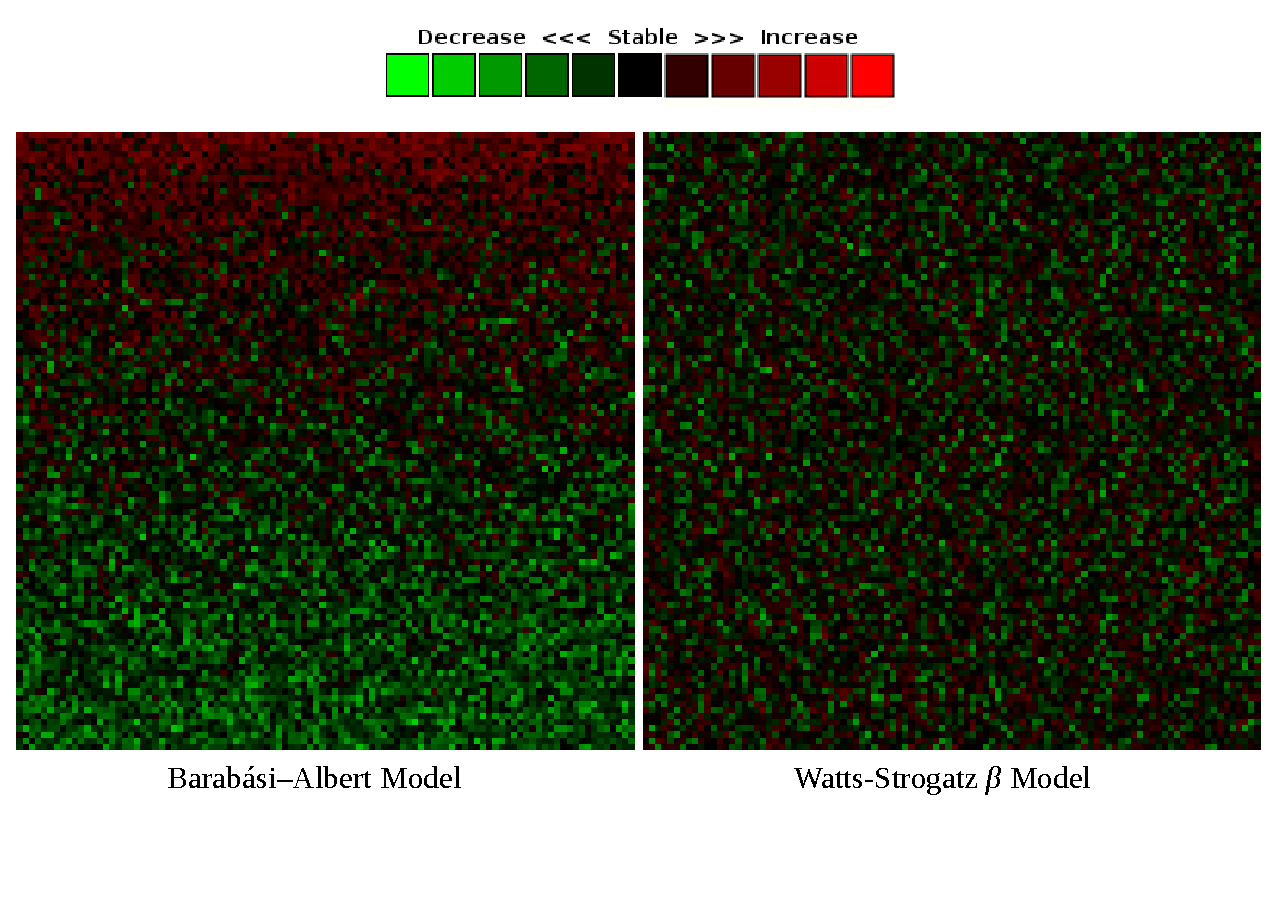
\includegraphics[width=0.87\textwidth]{figures/diffusion.pdf}
    \caption{Diffusion of Population} \label{fig:diffusion}
\end{figure}

\noindent
The LP state keeps track of the population residing in that location.  Individuals can leave one location and
travel to any of the connected locations.  The connections depends on the diffusion network layout.  The
following attributes are tracked in each individual:

\begin{itemize}
\item ID (unique for each individual in the entire population),
\item susceptibility to the disease (value $\in$ [0,1]),
\item vaccination status : \emph{yes / no}, and
\item \emph{PTTS} infection status (uninfected, latent, incubating, infectious, asympt or recovered). Refer to
  Figure \ref{fig:ptts} for details of the \emph{PTTS}.
\end{itemize}

\begin{figure}
  \centering
  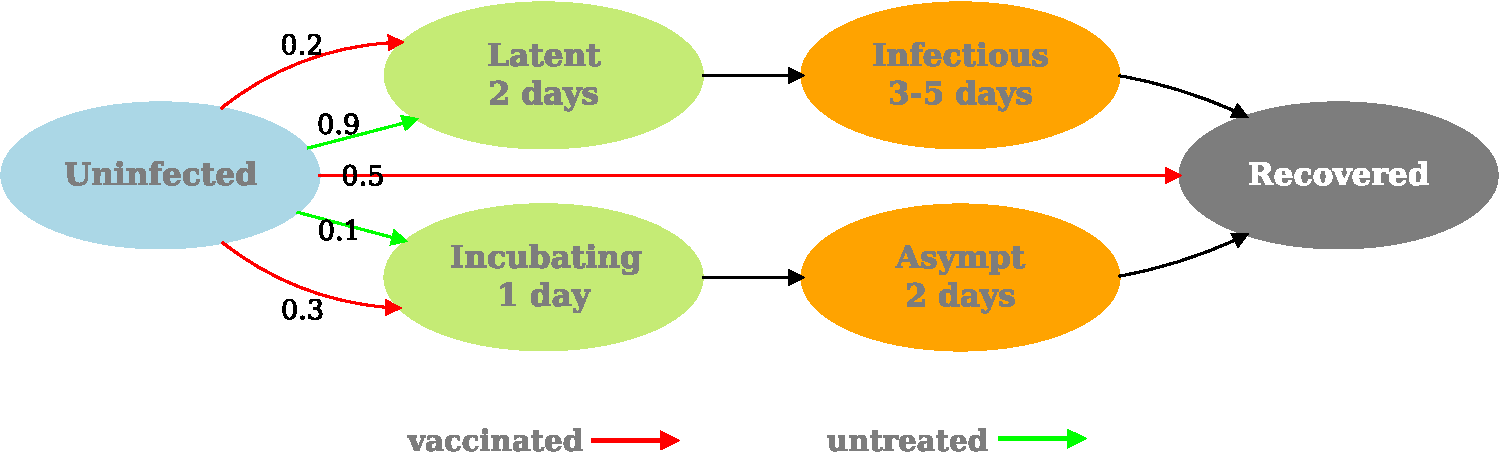
\includegraphics[width=0.85\textwidth]{figures/ptts.pdf}
  \caption{Probabilistic Timed Transition System}\label{fig:ptts}
\end{figure}

\begin{figure}
  \centering
  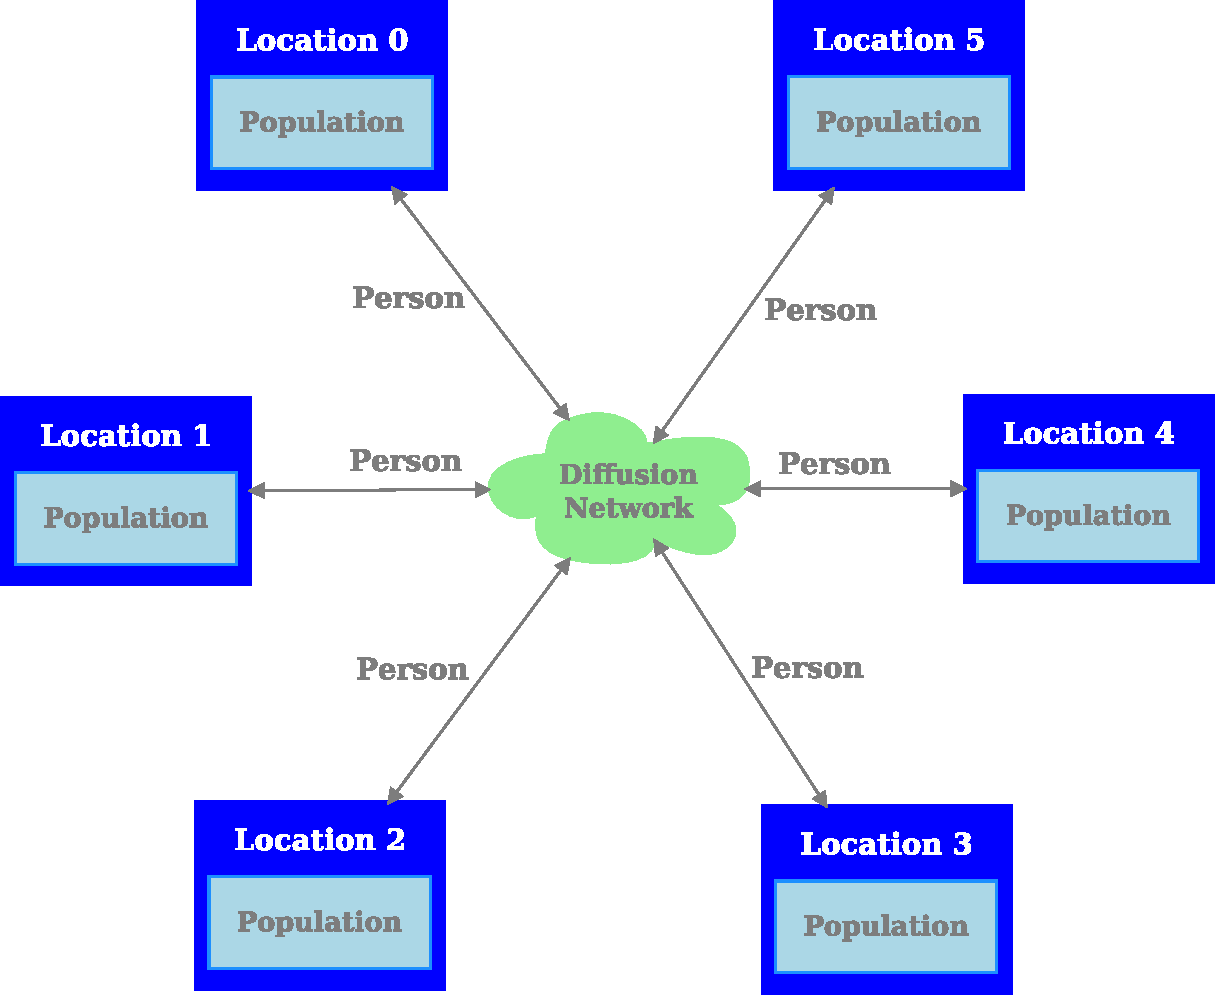
\includegraphics[width=0.75\textwidth]{figures/epidemic.pdf}
  \caption{Epidemic Model}\label{fig:epidemic}
\end{figure}

\noindent
An exponential distribution mimics the creation of events within the epidemic model.  The following are the
event types used in this simulation:

\begin{itemize}
\item \textbf{Disease Update Trigger}: self-initiated by the LP for updating the infection status of its
  resident population,
\item \textbf{Diffusion Trigger}: self-initiated by the LP for sending one resident to any neighboring
  location with uniform randomness, and
\item \textbf{Diffusion}: used when welcoming an arriving individual from a neighboring location.
\end{itemize}

Figure \ref{fig:epidemic} presents an illustration of the model.  Table \ref{table:epidemic_configs} shows the
different configurations of the epidemic model that have been used in Section \ref{sec:perf_analysis} and
appendix. Tables \ref{table:epidemic_10k_ws_config}, \ref{table:epidemic_10k_ba_config},
\ref{table:epidemic_100k_ws_config} and \ref{table:epidemic_100k_ba_config} provide the detailed configuration
for these models.

\begin{table}
    \centering
    \begin{tabular}{| l | c | c | r |}
        \hline
        \textbf{Configuration} & \textbf{Diffusion Network} & \textbf{Number of locations}
                & \textbf{Population}\\
        \hline
        epidemic-10k-ws     & Watts-Strogatz    &  10,000   & 1,000,000\\
        epidemic-10k-ba     & Barabasi-Albert   &  10,000   & 1,000,000\\
        epidemic-100k-ws    & Watts-Strogatz    &  100,000  & 500,000\\
        epidemic-100k-ba    & Barabasi-Albert   &  100,000  & 500,000\\
        \hline
    \end{tabular}
    \caption{List of Epidemic Configurations}\label{table:epidemic_configs}
\end{table}

\subsection{Portable Cellular Service (PCS)}\label{subsec:pcs}

This model simulates a wireless communication network capable of providing service to a number of subscribers
(or \emph{portables}).  The network service area comprises of \emph{cells}, each of which represents the
smallest building block in the simulation.  Each cell has a certain number of channels that can be used for
making or receiving calls.  Whenever there is an incoming or outgoing call, an available channel from the cell
is allocated.  In the event of channel unavailability, the call is \emph{blocked} \cite{lin-96-pcs}.  Each
cell represents a logical process in this simulation and they are organized as a rectangular grid (refer to
Figure \ref{fig:pcs}).  The test configuration uses a grid of size \emph{100 x 100} which translates to a LP
count of \emph{10,000}. Table \ref{table:pcs_10k_config} presents the configurations used for this model.

\begin{figure}
    \centering
    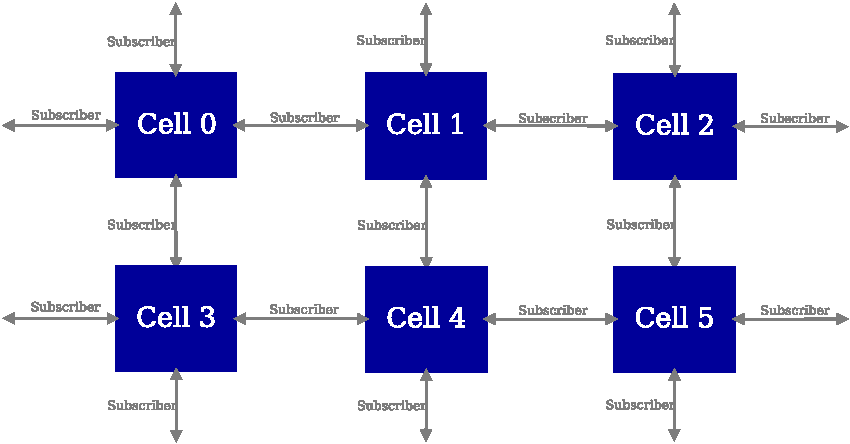
\includegraphics[width=0.9\textwidth]{figures/pcs.pdf}
    \caption{Portable Cellular Service Model}\label{fig:pcs}
\end{figure}

Portables can migrate to adjacent cells and there is a wrap around which occurs when a portable reaches one of
the edges.  Migration to an adjacent cell is a regular activity for portables and the time period is based on a
Poisson distribution.  A \emph{handoff block} happens for a migrating portable when the ongoing call is
dropped because all available channels are busy.  The state of Logical Process keeps track of the following
attributes for each cell:

\begin{itemize}
\item count of idle channels,
\item count of call attempts,
\item count of channel blocks, and
\item count of handoff blocks.
\end{itemize}

\noindent
Call requests to a portable follow a Poisson distribution.  The following are the types of events used in this
model:

\begin{itemize}
\item \emph{Next Call}: self-initiated by the cell to start a new call,
\item \emph{Call Completion}: self-initiated by the cell to set the call duration,
\item \emph{Portable Move Out}: self-initiated by the cell to send a portable to any of its adjacent cells
  with uniform randomness, and
\item \emph{Portable Move In}: receive a portable migrating from an adjacent cell.
\end{itemize}

\subsection{Traffic}\label{subsec:traffic}

The traffic model simulates how cars move through a grid of intersections in a city.  It models the nature of
traffic flow --- delays and choice of turns at intersections based on destination of the car.  The model
assumes that each road has three lanes in either direction and all intersections are four way.  This model has
been adapted from the \textsc{ROSS} \cite{carothers-00} simulator for \textsc{warped2}.

\begin{figure}
    \centering
    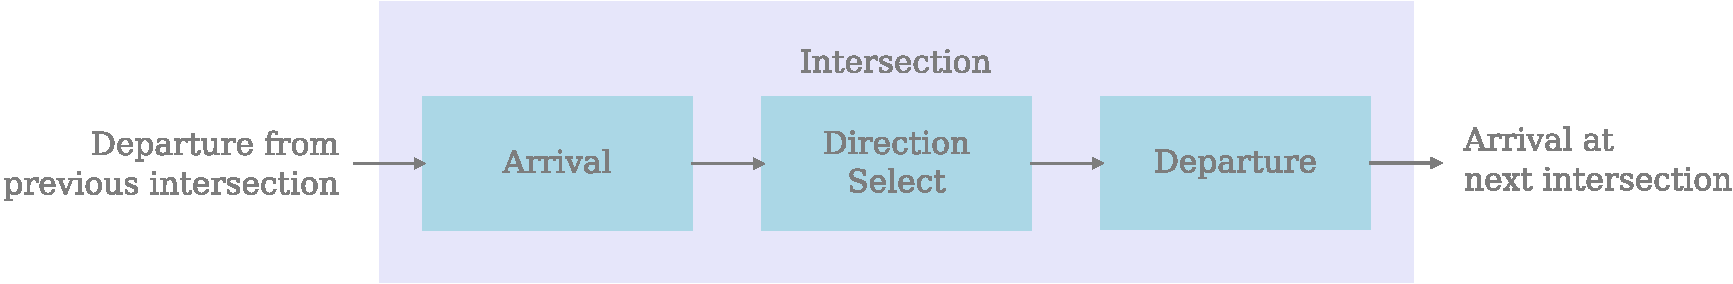
\includegraphics[width=1\textwidth]{figures/traffic_events.pdf}
    \caption{Sequence of events at each intersection}\label{fig:traffic_events}
\end{figure}

\noindent
Each intersection has been modeled as a Logical Processes and an event represents the movement
of cars through and between intersections.  Figure \ref{fig:traffic_events} shows the three
phases of an event at an intersection, namely :

\begin{itemize}
\item \emph{Arrival}: signifies the arrival of a car at an intersection from any of its adjacent intersection.
\item \emph{Direction Select} is a self-initiated event that helps the car to decide which direction to travel
  from the intersection it is currently at. This decision is based on the final destination the car is trying
  to reach and regulations controlling the flow of cars through that intersection.
\item \emph{Departure} is a self-initiated event which tells the intersection the car is currently located at
  that it is ready to travel to a different intersection.
\end{itemize}

The final destination for each car is a randomly assigned intersection.  At the initial stage, all available
cars are uniformly distributed across all intersections.  Once a car arrives at an intersection, it tries to
go in the direction that would get it closer to its target intersection.  There are thresholds in place to
help regulate and spread the flow of traffic.  This limits congestion on certain roads and may lead to a car
being denied permission to travel in the direction of its choice.  The car can randomly choose to either wait
or take an alternate route.  Events follow an exponential distribution and a new one is created when an
existing one is processed.

The status of traffic at each intersection at any point in time is tracked by the Logical Process state.  The
state has the following attributes which are used to decide whether a car can be allowed to travel in the
direction of its choice:

\begin{itemize}
\item number of cars arriving from each direction,
\item number of cars departing in each direction,
\item total number of cars arriving at the intersection, and
\item total number of cars departing from the intersection.
\end{itemize}

The grid has been modeled as a rectangular mesh to allow the traffic model to be scaled.  The traffic model in
\emph{ROSS} adopts a similar approach.  This grid arrangement is similar to the network structure used by
\emph{PCS} (as shown in Figure \ref{fig:pcs}).  Two configurations of traffic have been used for different
studies in this thesis.  Table \ref{table:traffic_configs} presents these two configurations and details for
each have been presented in Tables \ref{table:traffic_10k_config} and \ref{table:traffic_1m_config} respectively.

\begin{table}
    \centering
    \begin{tabular}{| l | c | r |}
        \hline
        \textbf{Configuration} & \textbf{Grid Dimension} & \textbf{Number of Cells}\\
        \hline
        traffic-10k     &  100 x 100    & 10,000\\
        traffic-1m      & 1024 x 1024   & 1,048,576\\
        \hline
    \end{tabular}
    \caption{List of Traffic Configurations}\label{table:traffic_configs}
\end{table}

\subsection{Abelian Sandpile}\label{subsec:sandpile}

The \emph{Abelian Sandpile} model or \emph{Bak-Tang-Wiesenfeld} model is a cellular automaton that is the
first discovered example of self-organized criticality in a dynamical system \cite{bak-87}.  The behavior is
considered Abelian because the final configuration is a function of the initial state, and is not affected by
the order in which the operations occur.  Each point on a finite square grid has an associated value which
represents the slope of the sandpile at that point.  This slope increases as "grains of sand" get randomly
added to the pile.  This growth continues till the slope exceeds a certain specified threshold at which point
it is considered unstable and it collapses.  This collapse transfers the collapsed sand equally to its
adjacent points, thereby increasing the slope of its neighbors.  The sand is steadily added to the center of
the grid and it spreads out in all directions due to the cascading behavior explained above.

Any point $(x,y)$ with $z(x,y) \geq 4$ is considered unstable and ready to topple.  That sends one grain of
sand to each of its four adjacent neighbors.  $z(x,y)$ represents the slope of the sandpile at point $(x,y)$.
The following equations represent how the sandpiles grow and collapse:

\begin{center}
  $z(x,y) \to z(x,y) - 4$\\
  $z(x\pm1,y) \to z(x\pm1,y) + 1$\\
  $z(x,y\pm1) \to z(x,y\pm1) + 1$\\
\end{center}

\noindent
Each point represents a logical process in the simulation. The state of each logical process has the following
attributes:

\begin{itemize}
\item height of the sandpile at point $(x,y)$ [ represented by $z(x,y)$ ], and
\item number of sandpile collapses at that point.
\end{itemize}

\begin{table}
    \centering
    \begin{tabular}{| l | c | r |}
        \hline
        \textbf{Configuration} & \textbf{Grid Dimension} & \textbf{Number of Cells}\\
        \hline
        sandpile-10k    & 100 x 100     & 10,000\\
        sandpile-1m     & 1000 x 1000   & 1,000,000\\
        \hline
    \end{tabular}
    \caption{List of Sandpile Configurations}\label{table:sandpile_configs}
\end{table}

\noindent
Table \ref{table:sandpile_configs} presents the test configurations used in this thesis. Tables
\ref{table:sandpile_10k_config} and \ref{table:sandpile_1m_config} presents a detailed view for each configuration.
Figure \ref{fig:sandpile} presents a magnified view of the output of an Abelian sandpile (sandpile-1m in Table
\ref{table:sandpile_configs}) where the colors indicate the slope of the points.

\begin{itemize}
\item \emph{Black}: point has never suffered a collapse and is empty,
\item \emph{Green}: point has collapsed in the past, but is now empty,
\item \emph{Yellow}: point with $slope = 1$,
\item \emph{Red}: point with $slope = 2$, and 
\item \emph{White}: point with $slope = 3$.
\end{itemize}

\begin{figure}
    \centering
    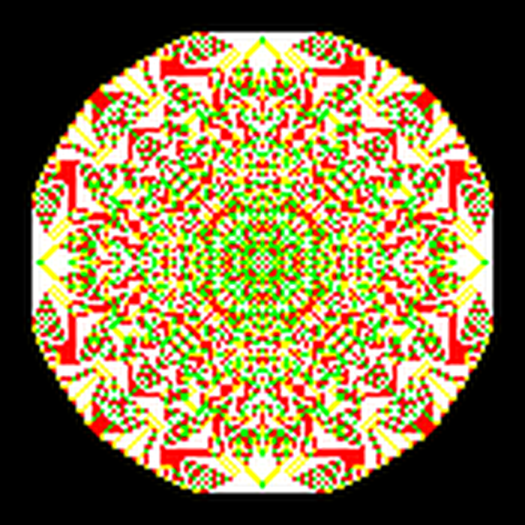
\includegraphics[width=0.5\textwidth]{figures/sandpile.pdf}
    \caption{Abelian Sandpile}\label{fig:sandpile}
\end{figure}


\section{Analysis of Performance}\label{sec:perf_analysis}

\subsection{Schedule Queue Data Structure}\label{subsec:scheduleq_type_plot}

This quantitative study is aimed at understanding the effectiveness of different data structures for storing
and scheduling events for execution in \textsc{warped-2}. The data structures being studied are STL MultiSet,
Splay Tree and Ladder Queue. Three separate variants of the Ladder Queue are under consideration, namely: (i)
one with a fully sorted Bottom and accessed with a mutex lock, (ii) one with an unsorted Bottom and accessed
with a mutex lock, and (iii) one with an unsorted Bottom that is accessed with a lock-free, atomic read-write
access setup.  The details for each data structure can be found in Section \ref{sec:data_structures}. In order
to eliminate the side-effects of load imbalance in this study, only a single schedule queue has been used. The
performance of these data structures for different thread counts (4, 8, 16, 32 and 64) has been
presented. Additional plots for multiple schedule queues with different data structures can be found in the
Appendix. Threshold is a critical parameter in Ladder Queue which triggers the split of a bucket when its
event count exceeds this threshold. Here three separate values of threshold have been studied, namely 16, 50
(as recommended by in \cite{tang-05}) and 96.

Figure \ref{plot:epidemic_10k_ba:scheduleq_type} (parts (a), (b), and (c)) show the performance impact of the
different data structures used for the Schedule Queue.  The number attached to the different Ladder Queue
variants in the plot keys represent the threshold of a Ladder Queue. The significant observations from these
plots have been explained below:

\begin{enumerate}

\item As expected, the Ladder Queue with Lock-free Unsorted Bottom outperforms the sorted Ladder Queue, Splay
  Tree and STL MultiSet by generally over 50\% as the number of worker threads increase.  However, it only
  marginally outperforms Ladder Queue with Unsorted Bottom.

\item In the original description of the Ladder Queue \cite{tang-05}, Tang \emph{et al} stipulate that the
  optimal value for threshold should be 50.  However, as can be seen in the performance data of Figure
  \ref{plot:epidemic_10k_ba:scheduleq_type}, the setting for this threshold has nominal impact on the overall
  performance. Section \ref{subsubsec:why_no_bottom_split} describes a modification to the original Ladder
  Queue algorithm which eliminates the need to split Bottom when its event count exceeds this threshold. This
  is probably why we don't see a huge variation in performance for the three threshold values. The penalty of
  this split would have been higher for a smaller threshold but there would be increased likelihood of causal
  violations when a larger threshold is used. It is likely that if this threshold value is increased further
  than 100, a point will be reached when this choice of threshold will start to negatively impact performance.
  This is because for that threshold value and beyond, the Ladder Queue will lose its ability to effectively
  put causally independent events into Bottom.

\item The Ladder Queue with an unsorted bottom is generally 50\% faster than the Ladder Queue with a sorted
  bottom.  This is expected because, in case of the former, no time is wasted on sorting events inside Bottom.
  The Event Commitment Ratio (Figure \ref{plot:epidemic_10k_ba:scheduleq_type}(b)) indicates there were no
  rollbacks in either case which means no time was lost due to recovery from causal violations.  The epidemic
  model generally tends to have low event density within a small time window.  This means sorting inside
  Bottom is not a significant overhead in case of this model.

\item The performance of most data structures marginally improves with increase in number of worker threads
  till about 16 threads and then marginally degrades. On the other hand, Ladder Queue with Lock-free Unsorted
  Bottom shows slight improvement in performance when thread count goes above 16. This is because atomic
  read-write operations are not affected adversely by increase in number of threads. However, the performance
  of other data structures here is surprising because contention for access to the shared Schedule Queue
  should increase with increase in number of worker threads. This should significantly degrade the performance
  as the thread count increases beyond 16 but that is not what has been observed. The architecture of the NUMA
  machine used may provide some clues. As mentioned in Table \ref{table:numa_setup}, each processor has 2
  sockets of 8 cores each and each core supports 2 hardware threads. This explains why the best performance is
  observed for 16 threads. However, it is difficult to speculate why the performance beyond 16 threads does
  not degrade significantly.

\end{enumerate}

\plotTrial{epidemic_10k_ba/plots/scheduleq/threads_vs_type_key_count_1}
          {Impact of the schedule queue data structure: Epidemic Model (\emph{10,000} LPs, \emph{Barabási-Albert} diffusion network)}
          {plot:epidemic_10k_ba:scheduleq_type}

\clearpage
Figure \ref{plot:epidemic_10k_ws:scheduleq_type} (parts (a), (b), and (c)) show that the performance
results of the Epidemic model with \emph{Watts-Strogatz}\cite{watts-98} diffusion network is
generally similar to that of Epidemic model with \emph{Barabási-Albert}\cite{barabasi-99} diffusion
network (shown in Figure \ref{plot:epidemic_10k_ba:scheduleq_type}).

\plotTrial{epidemic_10k_ws/plots/scheduleq/threads_vs_type_key_count_1}
          {Impact of the schedule queue data structure: Epidemic Model (\emph{10,000} LPs, \emph{Watts-Strogatz} diffusion network)}
          {plot:epidemic_10k_ws:scheduleq_type}

\clearpage
Compared to Epidemic Model plots in Figures \ref{plot:epidemic_10k_ba:scheduleq_type} and
\ref{plot:epidemic_10k_ws:scheduleq_type}, Traffic model behaves differently for Ladder Queue with
Lock-free Unsorted Bottom. Figure \ref{plot:traffic_10k:scheduleq_type} shows its performance is
nearly 90\% faster than Ladder Queue with Unsorted Bottom, which in turn is over 25\% faster than
sorted Ladder Queue. Traffic model tends to have higher event density within a small time window.
The simulation's performance benefits from not having to sort a large number of events that are
stored inside Bottom.

\plotTrial{traffic_10k/plots/scheduleq/threads_vs_type_key_count_1}
          {Impact of the schedule queue data structure: Traffic Model (\emph{10,000} LPs)}
          {plot:traffic_10k:scheduleq_type}

\clearpage
The PCS model, on the other hand, shows mixed performance for Ladder Queue with Lock-free Unsorted Bottom.  In
Figure \ref{plot:pcs_10k:scheduleq_type}, it starts off strongly but the performance tapers off with increase
in number of worker threads. Ladder Queue with Lock-Free Unsorted Bottom is still faster than its locked
counterpart but only by a small margin. Ladder Queue with Unsorted Bottom is around 20\% faster than sorted
Ladder Queue. Splay Tree is consistently the worst performer in every simulation model studied.

\plotTrial{pcs_10k/plots/scheduleq/threads_vs_type_key_count_1}
          {Impact of the schedule queue data structure: PCS Model (\emph{10,000} LPs)}
          {plot:pcs_10k:scheduleq_type}

\clearpage
\subsection{Multiple Schedule Queues}\label{subsec:scheduleq_count_plot}

This quantitative study aims to understand the impact of distributed event processing by multiple schedule
queues for different thread counts (4, 8, 16, 32 and 64). The schedule queue count never exceeds the thread count
because each schedule queue is allocated atleast one thread for processing its stored events. Detailed description
is available in Section \ref{subsec:multiple_scheduleq}. In order to retain clarity of presentation, only STL
MultiSet is used as the underlying schedule queue data structure. The performance impact of multiple schedule
queues when the underlying data structure is Splay Tree or Ladder Queue or any of its variants can be studied in
plots presented in the Appendix.

Figure \ref{plot:epidemic_10k_ba:scheduleq_count} shows the impact of partitioning the pending event set
uniformly across multiple Schedule Queues. Section \ref{subsec:multiple_scheduleq} explains this organization
in details. The plots show that performance improves steadily as the number of schedule queues is increased
up to 4, beyond which there is no further improvement. This is because there is a significant increase in
number of rollbacks when 8 or 16 schedule queues are used.

\plotTrial{epidemic_10k_ba/plots/scheduleq/threads_vs_count_key_type_stl-multiset}
          {Impact of the multiple schedule queues: Epidemic Model (\emph{10,000} LPs, \emph{Barabási-Albert} diffusion network)}
          {plot:epidemic_10k_ba:scheduleq_count}

\clearpage
Figure \ref{plot:epidemic_10k_ws:scheduleq_count} shows performance which is quite similar to that shown in
Figure \ref{plot:epidemic_10k_ba:scheduleq_count}, except for the low rollback count for higher number of
schedule queues. The low event event density within any time window of an epidemic model helps to preserve
better balance in a distributed simulation by not throwing rollbacks too frequently.

\plotTrial{epidemic_10k_ws/plots/scheduleq/threads_vs_count_key_type_stl-multiset}
          {Impact of the multiple schedule queues: Epidemic Model (\emph{10,000} LPs, \emph{Watts-Strogatz} diffusion network)}
          {plot:epidemic_10k_ws:scheduleq_count}

\clearpage
In comparison, Figure \ref{plot:traffic_10k:scheduleq_count} shows improvement in performance for
traffic model till the number of schedule queues is increased up to 8 beyond which there is no
further gain. The behavior of rollbacks here is a bit surprising given the reduction in their number
for thread count 32 and higher.

\plotTrial{traffic_10k/plots/scheduleq/threads_vs_count_key_type_stl-multiset}
          {Impact of the multiple schedule queues: Traffic Model (\emph{10,000} LPs)}
          {plot:traffic_10k:scheduleq_count}

\clearpage
Figure \ref{plot:pcs_10k:scheduleq_count} shows the performance of PCS model.  It is similar to that
of traffic model shown in Figure \ref{plot:traffic_10k:scheduleq_count}.

\plotTrial{pcs_10k/plots/scheduleq/threads_vs_count_key_type_stl-multiset}
          {Impact of the multiple schedule queues: PCS Model (\emph{10,000} LPs)}
          {plot:pcs_10k:scheduleq_count}

\clearpage
\subsection{Chain Scheduling}\label{subsec:chain_plot}

This quantitative analysis aims to study the effect of different chain sizes on the performance of
of \textsc{warped-2}. Section \ref{subsec:chains} presents a detailed description of event chain and
its size selection parameter. In order to simplify this analysis, only one schedule queue has been used
in order to avoid the adverse effects of load imbalance that often plagues simulations using multiple
schedule queues. The performance of \textsc{warped-2} when chains are used in combination with multiple
schedule queues can be studied from plots presented in the Appendix. The underlying data structure for
the schedule queue here is STL MultiSet and different thread counts used are 4, 8, 16, 32 and 64.

Figures \ref{plot:epidemic_10k_ba:chains} and \ref{plot:epidemic_10k_ws:chains} show the performance
of Epidemic model when chains of varying sizes are used. Both configurations of the model have
identical performance which remains fairly steady with increase in number of worker threads. Chain
size only has marginal effect on performance.  It is interesting to note that rollback count is
invariant for varying number of worker threads and fairly similar for different chain sizes. The
similar rollback count is likely because the local event chain size is mostly 1 (as shown in Figure
\ref{fig:local_event_chain:epidemic}). The performance of Chain Scheduling, which uses STL MultiSet
as Schedule Queue, is similar to that of a single Schedule Queue (shown in Figure
\ref{plot:epidemic_10k_ba:scheduleq_type}). Refer to Section \ref{subsec:chains} for a detailed
explanation of event chain.

\plotTrial{epidemic_10k_ba/plots/chains/threads_vs_chainsize_key_count_1}
          {Performance of Event Chains: Epidemic Model (\emph{10,000} LPs, \emph{Barabási-Albert} diffusion network)}
          {plot:epidemic_10k_ba:chains}

\plotTrial{epidemic_10k_ws/plots/chains/threads_vs_chainsize_key_count_1}
          {Performance of Event Chains: Epidemic Model (\emph{10,000} LPs, \emph{Watts-Strogatz} diffusion network)}
          {plot:epidemic_10k_ws:chains}

\newpage
Figure \ref{plot:traffic_10k:chains} shows that the performance of Traffic model with 10,000 LPs
remains invariant with change in chain size and worker thread count. Similar to Figures
\ref{plot:epidemic_10k_ba:chains} and \ref{plot:epidemic_10k_ws:chains}, rollback count is invariant
for varying number of worker threads but is significantly different for different chain sizes.

\plotTrial{traffic_10k/plots/chains/threads_vs_chainsize_key_count_1}
          {Performance of Event Chains: Traffic Model (\emph{10,000} LPs)}
          {plot:traffic_10k:chains}

For Traffic simulation with 1,048,576 LPs, Figure \ref{plot:traffic_1m:chains} shows
an unexpected loss of performance for 16 threads. The simulation is fairly stable for
other configurations.

\plotTrial{traffic_1m/plots/chains/threads_vs_chainsize_key_count_1}
          {Performance of Event Chains: Traffic Model (\emph{1,048,576} LPs)}
          {plot:traffic_1m:chains}

\clearpage
Figure \ref{plot:sandpile_10k:chains} shows the performance of chains for an Abelian Sandpile
simulation. The behavior observed here is significantly different from that observed for Epidemic
and Traffic models. The performance varies with increase in worker thread count. It is worst for 16
threads and improves drastically beyond that point. Rollback count also varies for different worker
thread count and chain sizes.  Similar to Traffic and Epidemic models, chain size does not have any
direct impact on performance.

\plotTrial{sandpile_10k/plots/chains/threads_vs_chainsize_key_count_1}
          {Performance of Event Chains: Abelian Sandpile Model (\emph{10,000} LPs)}
          {plot:sandpile_10k:chains}

\clearpage
\subsection{Block Scheduling}\label{subsec:block_plot}

This quantitative analysis aims to study the effect of different block sizes on the performance of
of \textsc{warped-2}. Section \ref{subsec:block_scheduling} presents a detailed description of blocks
and its size selection parameter. In order to simplify this analysis, only one schedule queue has been
used in order to avoid the adverse effects of load imbalance that often plagues simulations using
multiple schedule queues. The performance of \textsc{warped-2} when blocks are used in combination with
multiple schedule queues can be studied from plots presented in the Appendix. The underlying data
structure for the schedule queue here is STL MultiSet and different thread counts used are 4, 8, 16,
32 and 64.

Figures \ref{plot:epidemic_10k_ba:blocks} and \ref{plot:epidemic_10k_ws:blocks} show the performance
of Epidemic model when blocks of varying sizes are used. Both configurations of the model have
identical performance which remains fairly steady with increase in number of worker threads. Block
size only has marginal effect on performance.  It is interesting to note that block scheduling has
better performance when compared to that of chain scheduling. Refer to Section
\ref{subsec:block_scheduling} for a detailed explanation of event blocks.

\plotTrial{epidemic_10k_ba/plots/blocks/threads_vs_blocksize_key_count_1}
          {Performance of Event Blocks: Epidemic Model (\emph{10,000} LPs, \emph{Barabási-Albert} diffusion network)}
          {plot:epidemic_10k_ba:blocks}

\plotTrial{epidemic_10k_ws/plots/blocks/threads_vs_blocksize_key_count_1}
          {Performance of Event Blocks: Epidemic Model (\emph{10,000} LPs, \emph{Watts-Strogatz} diffusion network)}
          {plot:epidemic_10k_ws:blocks}

\clearpage
Figure \ref{plot:traffic_10k:blocks} shows that the performance of Traffic model with 10,000 LPs
remains invariant with change in block size and worker thread count.

\plotTrial{traffic_10k/plots/blocks/threads_vs_blocksize_key_count_1}
          {Performance of Event Blocks: Traffic Model (\emph{10,000} LPs)}
          {plot:traffic_10k:blocks}

\clearpage
Figure \ref{plot:traffic_1m:blocks} shows a Traffic simulation with 1,048,576 LPs behaves similar to
the 10,000 LP traffic simulation.

\plotTrial{traffic_1m/plots/blocks/threads_vs_blocksize_key_count_1}
          {Performance of Event Blocks: Traffic Model (\emph{1,048,576} LPs)}
          {plot:traffic_1m:blocks}

\newpage
Figure \ref{plot:sandpile_10k:blocks} shows the performance of blocks for an Abelian Sandpile
simulation. The behavior observed here is significantly different from that observed for Epidemic
and Traffic models. The performance varies with increase in worker thread count. It is mostly worst
for 16 threads and improves drastically beyond that point. Rollback count also varies for different
worker thread count and chain sizes. Unlike Traffic and Epidemic models, chain size does have a
major direct impact on performance.

\plotTrial{sandpile_10k/plots/blocks/threads_vs_blocksize_key_count_1}
          {Performance of Event Blocks: Abelian Sandpile Model (\emph{10,000} LPs)}
          {plot:sandpile_10k:blocks}

\newpage
\subsection{Bags with Static Window Size}\label{subsec:bags_static_window_plot}

In this study, the performance of bags and its static window size selection parameter are being
quantitatively analyzed. Section \ref{subsec:bags} presents a detailed description of bags. The
profile-driven partitioning for each benchmark model is driven by the event profile collected during
sequential simulation. Configuration for this sequential simulation can be found in the configuration
tables in the Appendix, namely Tables \ref{table:epidemic_10k_ws_config}, \ref{table:epidemic_100k_ws_config},
\ref{table:epidemic_10k_ba_config}, \ref{table:epidemic_100k_ba_config}, \ref{table:traffic_10k_config},
\ref{table:traffic_1m_config}, \ref{table:pcs_10k_config}, \ref{table:sandpile_10k_config} and
\ref{table:sandpile_1m_config}. The performance of \textsc{warped-2} is being evaluated for different
thread counts (4, 8, 16, 32 and 64) when using bags with different static window sizes, namely 4, 16,
32, 64, 128 and 256.

Figures \ref{plot:epidemic_10k_ba:bags:static_window} and
\ref{plot:epidemic_10k_ws:bags:static_window} show the performance of Epidemic Model where events
are scheduled from profile-driven LP partitions (refer to Section \ref{subsec:bags} for
details). Both configurations show fairly similar performance which peaks at 16 threads. From the
plots, it is evident that static window size has little or no impact up to thread count of
32. Similar to event chains, the rollback count remains invariant to increase in number of worker
threads and static window size. Epidemic model using Watts-Strogatz diffusion network has lesser
number of rollbacks compared to the Epidemic model using Barabasi-Albert diffusion network.  It is
worth noting that performance of bags is similar and sometimes superior to that of Ladder Queue with
Lock-free Unsorted Bottom in Figures \ref{plot:epidemic_10k_ba:scheduleq_type} and
\ref{plot:epidemic_10k_ws:scheduleq_type}.

\plotTrial{epidemic_10k_ba/plots/bags/threads_vs_staticwindow_key_fractionwindow_1.0}
          {Performance of Bags with Static Window Size: Epidemic Model (\emph{10,000} LPs, \emph{Barabási-Albert} diffusion network)}
          {plot:epidemic_10k_ba:bags:static_window}

\plotTrial{epidemic_10k_ws/plots/bags/threads_vs_staticwindow_key_fractionwindow_1.0}
          {Performance of Bags with Static Window Size: Epidemic Model (\emph{10,000} LPs, \emph{Watts-Strogatz} diffusion network)}
          {plot:epidemic_10k_ws:bags:static_window}

\clearpage
Figures \ref{plot:traffic_10k:bags:static_window} and \ref{plot:pcs_10k:bags:static_window} show the
performance of bags when using static window size for Traffic and PCS models respectively. Similar
to the behavior shown by the two different configurations of the Epidemic model, Traffic and PCS
models also have rollback count that remains invariant with increase in number of worker
threads. Peak performance is for 16 threads. The static window size parameter has very little or no
impact on the simulation.

\plotTrial{traffic_10k/plots/bags/threads_vs_staticwindow_key_fractionwindow_1.0}
          {Performance of Bags with Static Window Size: Traffic Model (\emph{10,000} LPs)}
          {plot:traffic_10k:bags:static_window}

\plotTrial{pcs_10k/plots/bags/threads_vs_staticwindow_key_fractionwindow_1.0}
          {Performance of Bags with Static Window Size: PCS Model (\emph{10,000} LPs)}
          {plot:pcs_10k:bags:static_window}

\clearpage
\subsection{Bags with Fractional Time Window}\label{subsec:bags_frac_window_plot}

Similar to Section \ref{subsec:bags_static_window_plot}, the performance of bags and its fractional window
selection parameter are being quantitatively analyzed in this study. The performance of \textsc{warped-2}
is being evaluated for different thread counts (4, 8, 16, 32 and 64) when using bags with fractional window.
The fractional parametric values evaluated are 0.05, 0.25, 0.50 and 0.75.

Figures \ref{plot:epidemic_10k_ba:bags:frac_time_window} and
\ref{plot:epidemic_10k_ws:bags:frac_time_window} show the performance of Epidemic Model where events
are scheduled from profile-driven LP partitions (refer to Section \ref{subsec:bags} for
details). Both configurations show fairly similar performance which peaks at 16 threads. From the
plots, it is evident that fraction of time window has little or no impact. Similar to event chains
and bags using static window size, the rollback count remains fairly invariant to increase in number
of worker threads and fraction of time window. Epidemic model using Watts-Strogatz diffusion network
has lesser number of rollbacks compared to the Epidemic model using Barabasi-Albert diffusion
network.

\plotTrial{epidemic_10k_ba/plots/bags/threads_vs_fractionwindow_key_staticwindow_0}
          {Performance of Bags with Fractional Time Window: Epidemic Model (\emph{10,000} LPs, \emph{Barabási-Albert} diffusion network)}
          {plot:epidemic_10k_ba:bags:frac_time_window}

\plotTrial{epidemic_10k_ws/plots/bags/threads_vs_fractionwindow_key_staticwindow_0}
          {Performance of Bags with Fractional Time Window: Epidemic Model (\emph{10,000} LPs, \emph{Watts-Strogatz} diffusion network)}
          {plot:epidemic_10k_ws:bags:frac_time_window}

\clearpage
Figures \ref{plot:traffic_10k:bags:frac_time_window} and \ref{plot:pcs_10k:bags:frac_time_window}
show the performance of bags when using fractional time window for Traffic and PCS models
respectively. Similar to the behavior shown by the two different configurations of the Epidemic
model, Traffic and PCS models also have rollback count that remains invariant with increase in
number of worker threads. Peak performance is for 16 threads. The fractional time window parameter
has very little or no impact on the simulation.

\plotTrial{traffic_10k/plots/bags/threads_vs_fractionwindow_key_staticwindow_0}
          {Performance of Bags with Fractional Time Window: Traffic Model (\emph{10,000} LPs)}
          {plot:traffic_10k:bags:frac_time_window}

\plotTrial{pcs_10k/plots/bags/threads_vs_fractionwindow_key_staticwindow_0}
          {Performance of Bags with Fractional Time Window: PCS Model (\emph{10,000} LPs)}
          {plot:pcs_10k:bags:frac_time_window}


\section{Summary of Performance Analysis}
\label{sec:analysis_summary}

Based on the data presented in Section \ref{sec:perf_analysis}, it can be observed that different
models react differently to the various options for schedule queue data structures and scheduling mechanisms.
In spite of these subtle differences in behavior, a common pattern does emerge. Ladder Queue with lock-free
access to unsorted bottom is generally the most efficient candidate for the schedule queue. Its event
processing rate is only eclipsed by multiple schedule queues. A possible configuration, therefore, can be
multiple schedule queues with each schedule queue being a Ladder Queue with Lockfree Unsorted Bottom. Figures
\ref{plot:traffic_10k:scheduleq:lockfree_ladderq} and \ref{plot:epidemic_10k_ws:scheduleq:lockfree_ladderq}
present the performance of the aforementioned configuration for two separate models. The network structure
and event density of these two models, namely Epidemic model with Watts-Strogatz network and Traffic model,
are different which should aid in model-specific comparisons. Since the threshold parameter in a Ladder Queue
has only negligible effect on simulation performance, threshold value of 96 is the only one used for this
presentation. Plots for multiple Ladder Queue-based schedule queues using Lockfree Unsorted Bottom and other
threshold values can be studied in the Appendix.

\plotTrial{traffic_10k/plots/scheduleq/threads_vs_count_key_type_lockfree-unsorted-bottom:96}
          {Traffic for Multiple Ladder Queue-based Schedule Queues with Lockfree Unsorted Bottom (\emph{10,000} LPs)}
          {plot:traffic_10k:scheduleq:lockfree_ladderq}

\plotTrial{epidemic_10k_ws/plots/scheduleq/threads_vs_count_key_type_lockfree-unsorted-bottom:96}
          {Epidemic (Watts-Strogatz network) for Multiple Ladder Queue-based Schedule Queues with Lockfree Unsorted Bottom (\emph{10,000} LPs)}
          {plot:epidemic_10k_ws:scheduleq:lockfree_ladderq}

Figure \ref{plot:traffic_10k:scheduleq:lockfree_ladderq} shows gain in performance for the traffic model when
compared against Figure \ref{plot:traffic_10k:scheduleq_count} (multiple STL MultiSet-based schedule queues )
or Figure \ref{plot:traffic_10k:scheduleq_type} (single schedule queue with different data structure options).
The gain is substantial when event processing rate is compared but marginal when simulation times are compared.

Figure \ref{plot:epidemic_10k_ws:scheduleq:lockfree_ladderq} shows gain in performance for the epidemic model
when compared against Figure \ref{plot:epidemic_10k_ws:scheduleq_count} (multiple STL MultiSet-based schedule
queues ) or Figure \ref{plot:epidemic_10k_ws:scheduleq_type} (single schedule queue with different data structure
options). The gain for event processing rate is marginal by comparison. Epidemic model has sparse event density
when compared to traffic model. This explains the increase in event processing rate for traffic. However, this
higher event density also increases the risk of causality violation in traffic. Infact there is a 5-10\%
increase in rollbacks for traffic while epidemic's rollback count increases by less than 1\%. As a result, any
performance gains in event processing rate for traffic is mostly cancelled by the increased number of rollbacks
it needs to take care of.


\chapter[Performance vs. Sequential]{Performance Comparison to Sequential Simulation}
\label{chapter:comparison_to_sequential}

\textbf{Speedup with respect to Sequential Simulation}, for a \textsc{warped-2} configuration, is a metric
used in this chapter to present a consolidated overview of the most effective scheduling data structures and
scheduling strategies found during the quantitative study presented in Chapter \ref{chapter:experiments} and
Appendix. The metric equals

\begin{equation*}
    \frac{\text{Time needed by Sequential Simulation to reach a certain timestamp}} {\text{Time needed by that
    Time Warp configuration to reach the same timestamp (or GVT)}}
\end{equation*}

\noindent
According to \cite{jefferson-91}, this speedup value represents the `supercritical speedup' of any
optimistically-synchronized parallel simulation such as \textsc{warped-2}.

\section[Quantitative Analysis]{Quantitative Analysis of Configurations}
\label{sec:qa_configurations}

\plotOverallNUMA{traffic_10k}
                {Top performers for Traffic (\emph{10,000} LPs) model}
                {plot:traffic_10k:consolidated}

\plotOverallNUMA{traffic_1m}
                {Top performers for Traffic (\emph{1,048,576} LPs) model}
                {plot:traffic_1m:consolidated}

\plotOverallNUMA{epidemic_10k_ba}
                {Top performers for Epidemic-BA (\emph{10,000} LPs) model}
                {plot:epidemic_10k_ba:consolidated}

\plotOverallNUMA{epidemic_10k_ws}
                {Top performers for Epidemic-WS (\emph{10,000} LPs) model}
                {plot:epidemic_10k_ws:consolidated}

\plotOverallNUMA{epidemic_100k_ba}
                {Top performers for Epidemic-BA (\emph{100,000} LPs) model}
                {plot:epidemic_100k_ba:consolidated}

\plotOverallNUMA{epidemic_100k_ws}
                {Top performers for Epidemic-WS (\emph{100,000} LPs) model}
                {plot:epidemic_100k_ws:consolidated}

\plotOverallNUMA{pcs_10k}
                {Top performers for PCS (\emph{10,000} LPs) model}
                {plot:pcs_10k:consolidated}

\plotOverallNUMA{sandpile_10k}
                {Top performers for Sandpile (\emph{10,000} LPs) model}
                {plot:sandpile_10k:consolidated}

\plotOverallNUMA{sandpile_1m}
                {Top performers for Sandpile (\emph{1,000,000} LPs) model}
                {plot:sandpile_1m:consolidated}

\subsection{Top Performers}
\label{subsec:top_performers}
Figures \ref{plot:traffic_10k:consolidated}(a) and \ref{plot:traffic_1m:consolidated}(a) show that
Ladder Queue with Lock-free Unsorted Bottom is a top performing configuration for the two Traffic
models. The choice of schedule queue count varies for the two models: 16 schedule queues is a top
performer for the 10,000 LPs Traffic model while 4 or 8 schedule queues work for the 1,000,000 LPs
Traffic model. Speedup against sequential simulation for both Traffic models are similar across a
range of scheduling techniques. The difference in schedule queue count is most likely due to higher
event processing ratio for the larger Traffic model.

Figures \ref{plot:sandpile_10k:consolidated}(a) and \ref{plot:sandpile_1m:consolidated}(a) show
massive speedup for the two Abelian Sandpile models (10,000 and 1,000,000 LPs respectively). Unlike
the Traffic models, both Sandpile models prefer one schedule queue and Ladder Queue with Lock-free
Unsorted Bottom is not a clear choice here. In general, all variants of Ladder Queue perform well
for both Sandpile models. This  of one schedule queue is a bit surprising and probably because
sandpile has the highest density of causally linked events because of its radially spreading network
structure.

Figure \ref{plot:pcs_10k:consolidated}(a) shows Ladder Queue with Lock-free Unsorted Bottom is the
clear choice for the PCS model. Similar to the Abelian Sandpile models, PCS seems to prefer one
schedule queue. It is most likely due to high causal event density like the Sandpile models. This
observation is significant because although both Traffic and PCS models use mesh network, their
performance window do not correlate so closely.

In case of the two Epidemic models with 10,000 LPs, the performance pattern looks strikingly
different when Epidemic with Watts-Strogatz network is compared to Epidemic with Barabasi-Albert
network. Figure \ref{plot:epidemic_10k_ws:consolidated}(a) shows block scheduling is quite effective
for Watts-Strogatz network but Figure \ref{plot:epidemic_10k_ba:consolidated}(a) shows Ladder Queue
with Lock-free Unsorted Bottom dominates for Barabasi-Albert network. The change in network structure
seems to drastically affect the density of causally-linked events. It can also be observed that it
is easier to pinpoint a good scheduling technique for Barabasi-Albert based Epidemic model when
compared to Watts-strogatz based model. In case of the latter model, many scheduling configurations
show good speedup.

Figures \ref{plot:epidemic_100k_ba:consolidated}(a) and \ref{plot:epidemic_100k_ws:consolidated}(a)
show that, for the Epidemic models with 100,000 LPs, Ladder Queue with Lock-free Unsorted Bottom is
the clear choice. Unlike Epidemic models with 10,000 LPs, both models here seem to prefer low number
of schedule queues (2, 4 and sometimes 8). The smaller 10,000 LPs Epidemic models prefer 8 or 16
schedule queues. In general, a wide variety of scheduling techniques work for the Watts-Strogatz
network while the preference is less wide for Barabasi-Albert based Epidemic simulation. Additionally,
Barabasi-Albert based Epidemic model prefers lower number of schedule queues. This is indicative of
higher density of causally linked events in case of the BA model. It explains why a wide variety of
scheduling techniques work for the WS model while the selection window is smaller for the BA model.

\subsubsection{Summary}
\label{subsubsec:summary_top}
The overwhelming choice for most models is Ladder Queue wih Lock-free Unsorted Bottom. Larger models
prefer lower schedule queue count (2,4 or maybe even 8) while smaller models generally work better
with higher number of schedule queues (8 or 16). Bags and chains are generally absent from the
95\texttt{th} percentile group for all models. In few cases like Traffic model, Block scheduling is a
powerful option as well. Additionally, the underlying network seems to play a key role in determining
which scheduling techniques are effective for a model, but PCS and Traffic defy this trend.


\subsection{Worst Performers}
\label{subsec:worst_performers}
Figures \ref{plot:traffic_10k:consolidated}(b), \ref{plot:traffic_1m:consolidated}(b),
\ref{plot:sandpile_10k:consolidated}(b), \ref{plot:sandpile_1m:consolidated}(b),
\ref{plot:pcs_10k:consolidated}(b), \ref{plot:epidemic_100k_ba:consolidated}(b) and
\ref{plot:epidemic_100k_ws:consolidated}(b) show that scheduling techniques in the lowest 10\texttt{th}
percentile are all slower than sequential simulation, except for Epidemic models with 10,000 LPs (Figures
\ref{plot:epidemic_10k_ba:consolidated}(b) and \ref{plot:epidemic_10k_ws:consolidated}(b)). Most
scheduling techniques (type of schedule queue, blocks and chains) use one schedule queue for a wide
variety of worker threads. It is expected that contention will slow down simulation but it is surprising
that the speedup is less than 1.

Chain and Bag scheduling techniques are some of the worst performers for the Epidemic models while
Chains perform slightly better than Block scheduling for the Sandpile models. The performance of Chain
scheduling suffers more than Block scheduling when LP count increases for Traffic and Sandpile models.
Both Chain and Block scheduling techniques perform very poorly for the 10,000 LP sized Traffic and
Sandpile models but performance of Block scheduling improves when LP count increases. Usually Block
scheduling techniques perform poorly for larger block sizes of 64, 128 or 256.

These observations for Chain, Bag and Block scheduling indicates that over-aggressive estimates of
causal independence are ineffective. The simulation models which suffer most from these over-aggressive
thresholds are Traffic, PCS and Abelian Sandpile - all have a higher density of causally-linked events
when compared to the Epidemic models.

\subsubsection{Summary}
\label{subsubsec:summary_worst}
The lowest 10\texttt{th} percentile results are good for understanding the effects of contention.
Since most of the scheduling techniques here use one schedule queue, we can assume load imbalance is
not an issue for the simulation models. This means only model-specific causal density and contention
can affect performance of different scheduling techniques. Epidemic models are of special interest here
because these models have the lowest density of causally-linked events. So contention for shared pending
event set is its primary hindrance for the Epidemic models. Based on observations from Figures
\ref{plot:epidemic_10k_ba:consolidated}(b) and \ref{plot:epidemic_10k_ws:consolidated}(b), Epidemic
models with 10,000 LPs suffer less than other models and shows speedup > 1. This observation indicates
that causal violations due to over-aggressive thresholds adversely affect performance equally or even
more than contention for the shared event pool.

\subsection{Anomalies in Performance}
\label{subsec:anomalies}

Figures \ref{plot:sandpile_10k:consolidated}(a) and \ref{plot:sandpile_1m:consolidated}(a) show unusually
high speedup values for the Abelian Sandpile model. Even Epidemic model with Barabasi-Albert network and
10,000 LPs shows high speedup values in Figure \ref{plot:epidemic_10k_ba:consolidated}(a). This behavior
indicates that some aspect of the processing architecture is making \textsc{warped-2} simulations extremely
efficient. Since these simulations were executed on NUMA-based computing platforms, the effect of distributed
caches is worth exploring. Section \ref{sec:smp_performance} presents a small study on a SMP node which
does not have such distributed cache arrangements. This study is useful for pinpointing that cache effects
in NUMA machines do play a major role in artificially boosting the performance of \textsc{warped-2}.

\section[WARPED-2 on SMP]{Performance of WARPED-2 on SMP machine}
\label{sec:smp_performance}

\begin{table}
    \centering
    \begin{tabular}{|| l | c | c ||}
    \hline
    & & Intel\textsuperscript{\textregistered} Xeon\textsuperscript{\textregistered}
            E5675\\ [0.5ex]
        \hline\hline
        \multirow{10}{*}{Processor}
            & ISA           & x86\_64   \\
            & \# Cores      & 6         \\
            & \# Threads    & 12        \\
            & \# Sockets    & 1         \\
            & Frequency     & 3.06 GHz  \\
            & Cache         & 12 MiB    \\
            & Memory        & 28 GB     \\
        \hline
        \multirow{7}{*}{Runtime}
            & OS Kernel         & 4.9.0-6-amd64           \\
            & C Library         & Debian GLIBC 2.24-11+deb9u3   \\ 
            & Compiler          & GCC v6.3.0                    \\
            & MPI               & MPICH v3.2                    \\
            & Python            & 2.7.13                        \\
            & Python-numpy      & 1.12.1                        \\
            & Python-networkx   & 1.11                          \\
        \hline
    \end{tabular}
    \caption{Experimental Setup for SMP machine}\label{table:smp_setup}
\end{table}

Figures \ref{plot:traffic_10k:consolidated_smp}, \ref{plot:traffic_1m:consolidated_smp},
\ref{plot:sandpile_10k:consolidated_smp}, \ref{plot:sandpile_1m:consolidated_smp},
\ref{plot:pcs_10k:consolidated_smp}, \ref{plot:epidemic_100k_ba:consolidated_smp},
\ref{plot:epidemic_100k_ws:consolidated_smp}, \ref{plot:epidemic_10k_ba:consolidated_smp} and
\ref{plot:epidemic_10k_ws:consolidated_smp} show the speedup vs. sequential simulation for all simulation
models. These simulations were executed on a SMP machine (refer to Table \ref{table:smp_setup}). All
configurations in these experiments use 6 worker threads because this study only aims to capture how cache
effects affect performance on a SMP machine when compared to a NUMA machine. Section \ref{subsec:anomalies}
presents the anomalies that exist in the data collected on the NUMA-based machines.

The following observations can be made from the data:

\begin{enumerate}
  \item The speedup numbers from the SMP machine are low for all simulation models. This indicates that
        the NUMA architecture is making the performance of \textsc{warped-2} look better in Section
        \ref{sec:qa_configurations} than it should have been.

  \item Ladder Queue with Lock-free Unsorted Bottom is generally the best option but not by a huge margin
        unlike what we observed from the NUMA experiments. That is partly due to use of lower number of
        threads (6) here. Locked queues do not suffer a lot from contention issues for lower thread count
        and so they tend to perform at a level comparable to Ladder Queue with Lock-free Unsorted Bottom
        when only 6 worker threads are used.

  \item The results show that 6 threads with 6 schedule queues is generally not a good option, mostly due
        to load imbalance which triggers too many rollbacks. The configurations that seem to perform well
        are 6 threads with 2 or 3 schedule queues. 

  \item Nearly all Time Warp configurations run slower than Sequential simulation for the Abelian Sandpile
        simulation model. This is surprising but, given the quadratic growth and unique radial spread in
        its network, it is possibly not a model well-suited for parallel simulation.
\end{enumerate}

\plotOverallSMP{traffic_10k}
               {Top performers for Traffic (\emph{10,000} LPs) model}
               {plot:traffic_10k:consolidated_smp}

\plotOverallSMP{traffic_1m}
               {Top performers for Traffic (\emph{1,048,576} LPs) model}
               {plot:traffic_1m:consolidated_smp}

\plotOverallSMP{epidemic_10k_ba}
               {Top performers for Epidemic-BA (\emph{10,000} LPs) model}
               {plot:epidemic_10k_ba:consolidated_smp}

\plotOverallSMP{epidemic_10k_ws}
               {Top performers for Epidemic-WS (\emph{10,000} LPs) model}
               {plot:epidemic_10k_ws:consolidated_smp}

\plotOverallSMP{epidemic_100k_ba}
               {Top performers for Epidemic-BA (\emph{100,000} LPs) model}
               {plot:epidemic_100k_ba:consolidated_smp}

\plotOverallSMP{epidemic_100k_ws}
               {Top performers for Epidemic-WS (\emph{100,000} LPs) model}
               {plot:epidemic_100k_ws:consolidated_smp}

\plotOverallSMP{pcs_10k}
               {Top performers for PCS (\emph{10,000} LPs) model}
               {plot:pcs_10k:consolidated_smp}

\plotOverallSMP{sandpile_10k}
               {Top performers for Sandpile (\emph{10,000} LPs) model}
               {plot:sandpile_10k:consolidated_smp}

\plotOverallSMP{sandpile_1m}
               {Top performers for Sandpile (\emph{1,000,000} LPs) model}
               {plot:sandpile_1m:consolidated_smp}



\chapter[Conclusion and Future Research]{Conclusions and Suggestions for Future Research}
\label{chapter:conclude}

\section{Conclusion}

This dissertation studies the problem of contention that prevents Time Warp-synchronized Parallel Discrete
Event Simulations from scaling up substantially on a multi-core computing platform.  The data structure that
holds the pending events is a major point of contention for threads trying to access and process these
scheduled events in parallel.  Several different data structures, namely STL MultiSet \cite{musser-89}, Splay
Tree \cite{sleator-85} and Ladder Queue \cite{tang-05}, have been explored and discussed in details.  The
Ladder Queue, a hierarchically organized priority queue, is of particular interest because of its ability to
self-split pending events into time-bound partitions without requiring any manual intervention like the
Calendar Queue \cite{brown-88}.  This self-split of pending events forces the smallest available events to
accumulate inside the lowest partition of the Ladder structure.  If one assumes that these events within the
lowest partition are causally independent, there is no further need to sort these events.  This approach saves
computational time otherwise wasted on sorting and also reduces contention to this shared pool by increasing
availability.  The contention can be further reduced through atomic read-write operations on this lowest
partition.  Experimental results presented in Section \ref{subsec:scheduleq_type_plot} show that atomic
operations on the unsorted lowest partition in a Ladder Queue improves performance of parallel simulation by
over 100\% when compared to a sorted Ladder Queue.

A parallel approach to contention management lies in exploration of alternative scheduling techniques.
Traditional PDES kernels maintain a common pending event pool which is accessed by threads for processing
events.  This organization prevents a simulation from scaling up massively on large multi-core computing
platforms.  Splitting this common pending event pool and distributing it uniformly among groups of threads was
successfully explored by Dickman \emph{et al} \cite{dickman-13}.  The benefit from reduction in contention
compensates for the extra rollbacks due to imbalance in distributed scheduling.  Experimental results
presented in Section \ref{subsec:scheduleq_count_plot} show that performance of simulation can be improved by
upto 150\% when the pending event pool is split into several pools, each having its own group of threads.

The combination of multiple schedule queues with each schedule queue being a Ladder Queue with lockfree
unsorted bottom is the best scheduling strategy for all simulation models studied in this thesis.  The gain in
performance from this configuration depends heavily on the event density of each model and tends to favor the
models with relatively high event density.  This is because this configuration improves the event processing
rate by reducing contention.  A models with high event density is ideally placed to benefit more from this
reduction in contention.  Section \ref{sec:analysis_summary} presents a detailed discussion on this topic.

Wilsey's \cite{wilsey-16} analysis of profile-driven data collected from Discrete Event Simulation showed that
it is possible for threads to schedule multiple events for processing without causing too many causal
violations.  Unlike traditional PDES where one event is scheduled at a time, scheduling multiple events at
once from a pending event pool reduces the overall time a thread wastes in waiting for access to this event
pool.  Gupta and Wilsey \cite{gupta-14} explored two different approaches: one where multiple events are
scheduled from a common pending event pool, and another where multiple events are scheduled from the LP that
holds the smallest unprocessed event.  Experimental results presented in Sections \ref{subsec:chain_plot} and
\ref{subsec:block_plot} show that this arrangement can speed up performance by upto 100\% for some simulation
models.  The results validate the findings in \cite{wilsey-16} that not all simulation models benefit from
events processed in groups.

Alt and Wilsey \cite{alt-14} showed that network statistics driven partitioning of LPs into `close-knit'
communities is effective for reducing remote messaging in a distributed environment.  This dissertation
explores the use of modularity-based techniques \cite{blondel-08} to partition LPs into dense communities
which are sparsely connected to other communities.  Section \ref{subsec:bags} explains that it is possible to
process a groups (or bag) of pending events from each community in parallel without drastic increase in number
of causal violations.  This arrangement extends the existing benefits of processing events in groups (as
discussed in the previous paragraph).  This organization also allows cyclic atomic scheduling of bags to a
waiting thread.  Experimental results presented in Sections \ref{subsec:bags_static_window_plot} and
\ref{subsec:bags_frac_window_plot} show that, for some models, the performance of bag scheduling technique
equals that of Ladder Queue with Lock-free Unsorted Bottom.


\section[Future Work]{Suggestions for Future Work}

\subsection{Hybrid Group Scheduling}

Sections \ref{subsec:chains} and \ref{subsec:block_scheduling} explain how events can be scheduled for
processing using chains and blocks respectively.  An idea that has not been explored in this dissertation
involves combining the two scheduling strategies together in order to schedule events from different LPs that
are within a bounding time window.  Event block can serve as the first-level filter for defining the bounding
time window.  Each LP within the block can then be allowed to schedule multiple events within this specified
time window for processing.  The assumption here would be that events within this time window are generally
causally independent of each other.

\subsection{Load Balancing on Multi-Core Processors}

For the past two decades, researchers have been exploring ways to balance workload in a Parallel Discrete
Event Simulation.  Several approaches have been proposed.  Deelman and Szymanski \cite{deelman-98} studied
dynamic load balancing for unbalanced simulation of spatially explicit problems.  Their proposed min-max based
approach balances the workload for a ring of processes by using an estimate for arrival time of future
events. Schlagenhaft \emph{et al} \cite{schlagenhaft-95} proposed that clusters of LPs can be moved between
processing elements.  Alt and Wilsey \cite{alt-14} showed that LPs can be partitioned using \textsc{metis}
\cite{karypis-98} and assigned to different nodes on a clusters by minimizing the number of remote events
communicated over the network.

The world of parallel computing has evolved significantly in the past two decades.  The advent of multi-core
processors has made it necessary to balance the workload distributed among threads within the same node.
Dickman \emph{et al} \cite{dickman-13} studied the problem of intra-node load balancing for multiple schedule
queues.  They proposed that LPs with the smallest events can migrate within a ring of schedule queues in order
to keep the simulation balanced and closer to the critical path. While this approach works well for some
simulation models, the design is sensitive to cache architecture of the host processor.  The performance of
such an arrangement is significantly poor on NUMA-based systems.  Linden \emph{et al} \cite{linden-18}
describes a similar load migration protocol for fine-grained dynamic load balancing, albeit one where LPs are
visualized as voxels.

In \textsc{warped2}, the pending events are partitioned and processed by several threads in parallel.  While
the event processing rate for each thread is approximately equal, the rate at which events are committed
varies for each thread.  Regulating the event processing rate across a group of threads may help keep the
simulation closer to the critical path.  This should reduce the number of rollbacks and result in an overall
improvement in simulation time.  Further research on this topic is required before arriving at a possible
solution.  An event profiler for Time Warp-based PDES may prove to be a valuable tool for this study.

\bibliography{refs}
\bibliographystyle{ieeetr} \markright{}

\appendix

\chapter[All Results]{Performance Results from all Configurations and Simulation Models}

Section \ref{sec:simulation_models} describes the different benchmarks used in the quantitative study of
different optimizations discussed in Chapter \ref{chapter:event_scheduling}. The following sections present
all the data collected for this study. Tables in each section provide configuration details for all benchmark
models.

\section[\textsc{traffic-10k lp}s]{Traffic Model Configured with 10,000 LPs}

Table \ref{table:traffic_10k_config} shows the configuration for this model.

\begin{table}
    \centering
    \begin{tabular}{|| l | r ||}
        \hline
        Parameter                           &   Values\\ [0.5ex]
        \hline\hline
        Number of Intersections (or LPs)    &   10,000\\
        Type of network connecting LPs      &   4-directional grid\\
        Grid Size                           &   100x100\\
        Number of Cars initially at each intersection   &   25\\
        Mean car arrival interval at each intersection  &   400 timestamp units\\
        Simulation Time                     &   10,000 timestamp units\\
        Sequential Simulation Time for calculating modularity   &   6000 timestamp units\\
        \hline
    \end{tabular}
    \caption{\textsc{Traffic Model} setup}\label{table:traffic_10k_config}
\end{table}

\plotTrialNoLabel{traffic_10k/plots/chains/threads_vs_count_key_chainsize_8}
                 {traffic 10k/plots/chains/threads vs count key chainsize 8}
\plotTrialNoLabel{traffic_10k/plots/chains/threads_vs_chainsize_key_count_1}
                 {traffic 10k/plots/chains/threads vs chainsize key count 1}
\plotTrialNoLabel{traffic_10k/plots/chains/threads_vs_chainsize_key_count_4}
                 {traffic 10k/plots/chains/threads vs chainsize key count 4}
\plotTrialNoLabel{traffic_10k/plots/chains/threads_vs_chainsize_key_count_16}
                 {traffic 10k/plots/chains/threads vs chainsize key count 16}
\plotTrialNoLabel{traffic_10k/plots/chains/threads_vs_count_key_chainsize_4}
                 {traffic 10k/plots/chains/threads vs count key chainsize 4}
\plotTrialNoLabel{traffic_10k/plots/chains/threads_vs_count_key_chainsize_12}
                 {traffic 10k/plots/chains/threads vs count key chainsize 12}
\plotTrialNoLabel{traffic_10k/plots/chains/threads_vs_chainsize_key_count_8}
                 {traffic 10k/plots/chains/threads vs chainsize key count 8}
\plotTrialNoLabel{traffic_10k/plots/chains/threads_vs_chainsize_key_count_2}
                 {traffic 10k/plots/chains/threads vs chainsize key count 2}
\plotTrialNoLabel{traffic_10k/plots/chains/threads_vs_count_key_chainsize_16}
                 {traffic 10k/plots/chains/threads vs count key chainsize 16}
\plotTrialNoLabel{traffic_10k/plots/scheduleq/threads_vs_count_key_type_ladder-queue:96}
                 {traffic 10k/plots/scheduleq/threads vs count key type ladder-queue 96}
\plotTrialNoLabel{traffic_10k/plots/scheduleq/threads_vs_count_key_type_stl-multiset}
                 {traffic 10k/plots/scheduleq/threads vs count key type stl-multiset}
\plotTrialNoLabel{traffic_10k/plots/scheduleq/threads_vs_count_key_type_unsorted-bottom:50}
                 {traffic 10k/plots/scheduleq/threads vs count key type unsorted-bottom 50}
\plotTrialNoLabel{traffic_10k/plots/scheduleq/threads_vs_count_key_type_lockfree-unsorted-bottom:50}
                 {traffic 10k/plots/scheduleq/threads vs count key type lockfree-unsorted-bottom 50}
\plotTrialNoLabel{traffic_10k/plots/scheduleq/threads_vs_type_key_count_16}
                 {traffic 10k/plots/scheduleq/threads vs type key count 16}
\plotTrialNoLabel{traffic_10k/plots/scheduleq/threads_vs_type_key_count_4}
                 {traffic 10k/plots/scheduleq/threads vs type key count 4}
\plotTrialNoLabel{traffic_10k/plots/scheduleq/threads_vs_count_key_type_lockfree-unsorted-bottom:96}
                 {traffic 10k/plots/scheduleq/threads vs count key type lockfree-unsorted-bottom 96}
\plotTrialNoLabel{traffic_10k/plots/scheduleq/threads_vs_count_key_type_splay-tree}
                 {traffic 10k/plots/scheduleq/threads vs count key type splay-tree}
\plotTrialNoLabel{traffic_10k/plots/scheduleq/threads_vs_count_key_type_unsorted-bottom:96}
                 {traffic 10k/plots/scheduleq/threads vs count key type unsorted-bottom 96}
\plotTrialNoLabel{traffic_10k/plots/scheduleq/threads_vs_count_key_type_ladder-queue:50}
                 {traffic 10k/plots/scheduleq/threads vs count key type ladder-queue 50}
\plotTrialNoLabel{traffic_10k/plots/scheduleq/threads_vs_type_key_count_8}
                 {traffic 10k/plots/scheduleq/threads vs type key count 8}
\plotTrialNoLabel{traffic_10k/plots/scheduleq/threads_vs_count_key_type_lockfree-unsorted-bottom:16}
                 {traffic 10k/plots/scheduleq/threads vs count key type lockfree-unsorted-bottom 16}
\plotTrialNoLabel{traffic_10k/plots/scheduleq/threads_vs_type_key_count_2}
                 {traffic 10k/plots/scheduleq/threads vs type key count 2}
\plotTrialNoLabel{traffic_10k/plots/scheduleq/threads_vs_count_key_type_ladder-queue:16}
                 {traffic 10k/plots/scheduleq/threads vs count key type ladder-queue 16}
\plotTrialNoLabel{traffic_10k/plots/scheduleq/threads_vs_type_key_count_1}
                 {traffic 10k/plots/scheduleq/threads vs type key count 1}
\plotTrialNoLabel{traffic_10k/plots/scheduleq/threads_vs_count_key_type_unsorted-bottom:16}
                 {traffic 10k/plots/scheduleq/threads vs count key type unsorted-bottom 16}
\plotTrialNoLabel{traffic_10k/plots/bags/threads_vs_staticwindow_key_fractionwindow_1.0}
                 {traffic 10k/plots/bags/threads vs staticwindow key fractionwindow 1.0}
\plotTrialNoLabel{traffic_10k/plots/bags/threads_vs_fractionwindow_key_staticwindow_0}
                 {traffic 10k/plots/bags/threads vs fractionwindow key staticwindow 0}
\plotTrialNoLabel{traffic_10k/plots/blocks/threads_vs_blocksize_key_count_4}
                 {traffic 10k/plots/blocks/threads vs blocksize key count 4}
\plotTrialNoLabel{traffic_10k/plots/blocks/threads_vs_blocksize_key_count_2}
                 {traffic 10k/plots/blocks/threads vs blocksize key count 2}
\plotTrialNoLabel{traffic_10k/plots/blocks/threads_vs_count_key_blocksize_256}
                 {traffic 10k/plots/blocks/threads vs count key blocksize 256}
\plotTrialNoLabel{traffic_10k/plots/blocks/threads_vs_blocksize_key_count_8}
                 {traffic 10k/plots/blocks/threads vs blocksize key count 8}
\plotTrialNoLabel{traffic_10k/plots/blocks/threads_vs_count_key_blocksize_32}
                 {traffic 10k/plots/blocks/threads vs count key blocksize 32}
\plotTrialNoLabel{traffic_10k/plots/blocks/threads_vs_blocksize_key_count_16}
                 {traffic 10k/plots/blocks/threads vs blocksize key count 16}
\plotTrialNoLabel{traffic_10k/plots/blocks/threads_vs_blocksize_key_count_1}
                 {traffic 10k/plots/blocks/threads vs blocksize key count 1}
\plotTrialNoLabel{traffic_10k/plots/blocks/threads_vs_count_key_blocksize_128}
                 {traffic 10k/plots/blocks/threads vs count key blocksize 128}
\plotTrialNoLabel{traffic_10k/plots/blocks/threads_vs_count_key_blocksize_64}
                 {traffic 10k/plots/blocks/threads vs count key blocksize 64}

\clearpage
\section[\textsc{traffic-1m lp}s]{Traffic Model Configured with 1,048,576 LPs}

Table \ref{table:traffic_1m_config} shows the configuration for this model.

\begin{table}
    \centering
    \begin{tabular}{|| l | r ||}
        \hline
        Parameter                           &   Values\\ [0.5ex]
        \hline\hline
        Number of Intersections (or LPs)    &   1,048,576\\
        Type of network connecting LPs      &   4-directional grid\\
        Grid Size                           &   1024x1024\\
        Number of Cars initially at each intersection   &   25\\
        Mean car arrival interval at each intersection  &   400 timestamp units\\
        Simulation Time                     &   500 timestamp units\\
        Sequential Simulation Time for calculating modularity   &   300 timestamp units\\
        \hline
    \end{tabular}
    \caption{\textsc{Large Traffic Model} setup}\label{table:traffic_1m_config}
\end{table}

\plotTrialNoLabel{traffic_1m/plots/chains/threads_vs_count_key_chainsize_8}
                 {traffic 1m/plots/chains/threads vs count key chainsize 8}
\plotTrialNoLabel{traffic_1m/plots/chains/threads_vs_chainsize_key_count_1}
                 {traffic 1m/plots/chains/threads vs chainsize key count 1}
\plotTrialNoLabel{traffic_1m/plots/chains/threads_vs_chainsize_key_count_4}
                 {traffic 1m/plots/chains/threads vs chainsize key count 4}
\plotTrialNoLabel{traffic_1m/plots/chains/threads_vs_chainsize_key_count_16}
                 {traffic 1m/plots/chains/threads vs chainsize key count 16}
\plotTrialNoLabel{traffic_1m/plots/chains/threads_vs_count_key_chainsize_4}
                 {traffic 1m/plots/chains/threads vs count key chainsize 4}
\plotTrialNoLabel{traffic_1m/plots/chains/threads_vs_count_key_chainsize_12}
                 {traffic 1m/plots/chains/threads vs count key chainsize 12}
\plotTrialNoLabel{traffic_1m/plots/chains/threads_vs_chainsize_key_count_8}
                 {traffic 1m/plots/chains/threads vs chainsize key count 8}
\plotTrialNoLabel{traffic_1m/plots/chains/threads_vs_chainsize_key_count_2}
                 {traffic 1m/plots/chains/threads vs chainsize key count 2}
\plotTrialNoLabel{traffic_1m/plots/chains/threads_vs_count_key_chainsize_16}
                 {traffic 1m/plots/chains/threads vs count key chainsize 16}
\plotTrialNoLabel{traffic_1m/plots/scheduleq/threads_vs_count_key_type_stl-multiset}
                 {traffic 1m/plots/scheduleq/threads vs count key type stl-multiset}
\plotTrialNoLabel{traffic_1m/plots/scheduleq/threads_vs_count_key_type_lockfree-unsorted-bottom:50}
                 {traffic 1m/plots/scheduleq/threads vs count key type lockfree-unsorted-bottom 50}
\plotTrialNoLabel{traffic_1m/plots/scheduleq/threads_vs_type_key_count_16}
                 {traffic 1m/plots/scheduleq/threads vs type key count 16}
\plotTrialNoLabel{traffic_1m/plots/scheduleq/threads_vs_type_key_count_4}
                 {traffic 1m/plots/scheduleq/threads vs type key count 4}
\plotTrialNoLabel{traffic_1m/plots/scheduleq/threads_vs_count_key_type_lockfree-unsorted-bottom:96}
                 {traffic 1m/plots/scheduleq/threads vs count key type lockfree-unsorted-bottom 96}
\plotTrialNoLabel{traffic_1m/plots/scheduleq/threads_vs_count_key_type_splay-tree}
                 {traffic 1m/plots/scheduleq/threads vs count key type splay-tree}
\plotTrialNoLabel{traffic_1m/plots/scheduleq/threads_vs_type_key_count_8}
                 {traffic 1m/plots/scheduleq/threads vs type key count 8}
\plotTrialNoLabel{traffic_1m/plots/scheduleq/threads_vs_count_key_type_lockfree-unsorted-bottom:16}
                 {traffic 1m/plots/scheduleq/threads vs count key type lockfree-unsorted-bottom 16}
\plotTrialNoLabel{traffic_1m/plots/scheduleq/threads_vs_type_key_count_2}
                 {traffic 1m/plots/scheduleq/threads vs type key count 2}
\plotTrialNoLabel{traffic_1m/plots/scheduleq/threads_vs_type_key_count_1}
                 {traffic 1m/plots/scheduleq/threads vs type key count 1}
\plotTrialNoLabel{traffic_1m/plots/blocks/threads_vs_blocksize_key_count_4}
                 {traffic 1m/plots/blocks/threads vs blocksize key count 4}
\plotTrialNoLabel{traffic_1m/plots/blocks/threads_vs_blocksize_key_count_2}
                 {traffic 1m/plots/blocks/threads vs blocksize key count 2}
\plotTrialNoLabel{traffic_1m/plots/blocks/threads_vs_count_key_blocksize_256}
                 {traffic 1m/plots/blocks/threads vs count key blocksize 256}
\plotTrialNoLabel{traffic_1m/plots/blocks/threads_vs_blocksize_key_count_8}
                 {traffic 1m/plots/blocks/threads vs blocksize key count 8}
\plotTrialNoLabel{traffic_1m/plots/blocks/threads_vs_count_key_blocksize_32}
                 {traffic 1m/plots/blocks/threads vs count key blocksize 32}
\plotTrialNoLabel{traffic_1m/plots/blocks/threads_vs_blocksize_key_count_16}
                 {traffic 1m/plots/blocks/threads vs blocksize key count 16}
\plotTrialNoLabel{traffic_1m/plots/blocks/threads_vs_blocksize_key_count_1}
                 {traffic 1m/plots/blocks/threads vs blocksize key count 1}
\plotTrialNoLabel{traffic_1m/plots/blocks/threads_vs_count_key_blocksize_128}
                 {traffic 1m/plots/blocks/threads vs count key blocksize 128}
\plotTrialNoLabel{traffic_1m/plots/blocks/threads_vs_count_key_blocksize_64}
                 {traffic 1m/plots/blocks/threads vs count key blocksize 64}

\clearpage
\section[\textsc{epidemic-ws-10k lp}s]{Epidemic Model with 10,000 LPs and Watts-Strogatz Network}

Table \ref{table:epidemic_10k_ws_config} shows the configuration for this model.

\begin{table}
    \centering
    \begin{tabular}{|| l | r ||}
        \hline
        Parameter                           &   Values\\ [0.5ex]
        \hline\hline
        Number of Intersections (or LPs)    &   10,000\\
        Type of network connecting LPs      &   Watts-Strogatz \cite{watts-98}\\
        Population Size                     &   1,000,000\\
        Simulation Time                     &   15,000 timestamp units\\
        Sequential Simulation Time for calculating modularity   &   8,000 timestamp units\\
        \hline
    \end{tabular}
    \caption{\textsc{Epidemic Model with Watts-Strogatz} setup}\label{table:epidemic_10k_ws_config}
\end{table}

\plotTrialNoLabel{epidemic_10k_ws/plots/chains/threads_vs_count_key_chainsize_8}
                 {epidemic 10k ws/plots/chains/threads vs count key chainsize 8}
\plotTrialNoLabel{epidemic_10k_ws/plots/chains/threads_vs_chainsize_key_count_1}
                 {epidemic 10k ws/plots/chains/threads vs chainsize key count 1}
\plotTrialNoLabel{epidemic_10k_ws/plots/chains/threads_vs_chainsize_key_count_4}
                 {epidemic 10k ws/plots/chains/threads vs chainsize key count 4}
\plotTrialNoLabel{epidemic_10k_ws/plots/chains/threads_vs_chainsize_key_count_16}
                 {epidemic 10k ws/plots/chains/threads vs chainsize key count 16}
\plotTrialNoLabel{epidemic_10k_ws/plots/chains/threads_vs_count_key_chainsize_4}
                 {epidemic 10k ws/plots/chains/threads vs count key chainsize 4}
\plotTrialNoLabel{epidemic_10k_ws/plots/chains/threads_vs_count_key_chainsize_12}
                 {epidemic 10k ws/plots/chains/threads vs count key chainsize 12}
\plotTrialNoLabel{epidemic_10k_ws/plots/chains/threads_vs_chainsize_key_count_8}
                 {epidemic 10k ws/plots/chains/threads vs chainsize key count 8}
\plotTrialNoLabel{epidemic_10k_ws/plots/chains/threads_vs_chainsize_key_count_2}
                 {epidemic 10k ws/plots/chains/threads vs chainsize key count 2}
\plotTrialNoLabel{epidemic_10k_ws/plots/chains/threads_vs_count_key_chainsize_16}
                 {epidemic 10k ws/plots/chains/threads vs count key chainsize 16}
\plotTrialNoLabel{epidemic_10k_ws/plots/scheduleq/threads_vs_count_key_type_ladder-queue:96}
                 {epidemic 10k ws/plots/scheduleq/threads vs count key type ladder-queue 96}
\plotTrialNoLabel{epidemic_10k_ws/plots/scheduleq/threads_vs_count_key_type_stl-multiset}
                 {epidemic 10k ws/plots/scheduleq/threads vs count key type stl-multiset}
\plotTrialNoLabel{epidemic_10k_ws/plots/scheduleq/threads_vs_count_key_type_unsorted-bottom:50}
                 {epidemic 10k ws/plots/scheduleq/threads vs count key type unsorted-bottom 50}
\plotTrialNoLabel{epidemic_10k_ws/plots/scheduleq/threads_vs_count_key_type_lockfree-unsorted-bottom:50}
                 {epidemic 10k ws/plots/scheduleq/threads vs count key type lockfree-unsorted-bottom 50}
\plotTrialNoLabel{epidemic_10k_ws/plots/scheduleq/threads_vs_type_key_count_16}
                 {epidemic 10k ws/plots/scheduleq/threads vs type key count 16}
\plotTrialNoLabel{epidemic_10k_ws/plots/scheduleq/threads_vs_type_key_count_4}
                 {epidemic 10k ws/plots/scheduleq/threads vs type key count 4}
\plotTrialNoLabel{epidemic_10k_ws/plots/scheduleq/threads_vs_count_key_type_lockfree-unsorted-bottom:96}
                 {epidemic 10k ws/plots/scheduleq/threads vs count key type lockfree-unsorted-bottom 96}
\plotTrialNoLabel{epidemic_10k_ws/plots/scheduleq/threads_vs_count_key_type_splay-tree}
                 {epidemic 10k ws/plots/scheduleq/threads vs count key type splay-tree}
\plotTrialNoLabel{epidemic_10k_ws/plots/scheduleq/threads_vs_count_key_type_unsorted-bottom:96}
                 {epidemic 10k ws/plots/scheduleq/threads vs count key type unsorted-bottom 96}
\plotTrialNoLabel{epidemic_10k_ws/plots/scheduleq/threads_vs_count_key_type_ladder-queue:50}
                 {epidemic 10k ws/plots/scheduleq/threads vs count key type ladder-queue 50}
\plotTrialNoLabel{epidemic_10k_ws/plots/scheduleq/threads_vs_type_key_count_8}
                 {epidemic 10k ws/plots/scheduleq/threads vs type key count 8}
\plotTrialNoLabel{epidemic_10k_ws/plots/scheduleq/threads_vs_count_key_type_lockfree-unsorted-bottom:16}
                 {epidemic 10k ws/plots/scheduleq/threads vs count key type lockfree-unsorted-bottom 16}
\plotTrialNoLabel{epidemic_10k_ws/plots/scheduleq/threads_vs_type_key_count_2}
                 {epidemic 10k ws/plots/scheduleq/threads vs type key count 2}
\plotTrialNoLabel{epidemic_10k_ws/plots/scheduleq/threads_vs_count_key_type_ladder-queue:16}
                 {epidemic 10k ws/plots/scheduleq/threads vs count key type ladder-queue 16}
\plotTrialNoLabel{epidemic_10k_ws/plots/scheduleq/threads_vs_type_key_count_1}
                 {epidemic 10k ws/plots/scheduleq/threads vs type key count 1}
\plotTrialNoLabel{epidemic_10k_ws/plots/scheduleq/threads_vs_count_key_type_unsorted-bottom:16}
                 {epidemic 10k ws/plots/scheduleq/threads vs count key type unsorted-bottom 16}
\plotTrialNoLabel{epidemic_10k_ws/plots/bags/threads_vs_staticwindow_key_fractionwindow_1.0}
                 {epidemic 10k ws/plots/bags/threads vs staticwindow key fractionwindow 1.0}
\plotTrialNoLabel{epidemic_10k_ws/plots/bags/threads_vs_fractionwindow_key_staticwindow_0}
                 {epidemic 10k ws/plots/bags/threads vs fractionwindow key staticwindow 0}
\plotTrialNoLabel{epidemic_10k_ws/plots/blocks/threads_vs_blocksize_key_count_4}
                 {epidemic 10k ws/plots/blocks/threads vs blocksize key count 4}
\plotTrialNoLabel{epidemic_10k_ws/plots/blocks/threads_vs_blocksize_key_count_2}
                 {epidemic 10k ws/plots/blocks/threads vs blocksize key count 2}
\plotTrialNoLabel{epidemic_10k_ws/plots/blocks/threads_vs_count_key_blocksize_256}
                 {epidemic 10k ws/plots/blocks/threads vs count key blocksize 256}
\plotTrialNoLabel{epidemic_10k_ws/plots/blocks/threads_vs_blocksize_key_count_8}
                 {epidemic 10k ws/plots/blocks/threads vs blocksize key count 8}
\plotTrialNoLabel{epidemic_10k_ws/plots/blocks/threads_vs_count_key_blocksize_32}
                 {epidemic 10k ws/plots/blocks/threads vs count key blocksize 32}
\plotTrialNoLabel{epidemic_10k_ws/plots/blocks/threads_vs_blocksize_key_count_16}
                 {epidemic 10k ws/plots/blocks/threads vs blocksize key count 16}
\plotTrialNoLabel{epidemic_10k_ws/plots/blocks/threads_vs_blocksize_key_count_1}
                 {epidemic 10k ws/plots/blocks/threads vs blocksize key count 1}
\plotTrialNoLabel{epidemic_10k_ws/plots/blocks/threads_vs_count_key_blocksize_128}
                 {epidemic 10k ws/plots/blocks/threads vs count key blocksize 128}
\plotTrialNoLabel{epidemic_10k_ws/plots/blocks/threads_vs_count_key_blocksize_64}
                 {epidemic 10k ws/plots/blocks/threads vs count key blocksize 64}

\clearpage
\section[\textsc{epidemic-ws-100k lp}s]{Epidemic Model with 100,000 LPs and Watts-Strogatz Network}

Table \ref{table:epidemic_100k_ws_config} shows the configuration for this model.

\begin{table}
    \centering
    \begin{tabular}{|| l | r ||}
        \hline
        Parameter                           &   Values\\ [0.5ex]
        \hline\hline
        Number of Intersections (or LPs)    &   100,000\\
        Type of network connecting LPs      &   Watts-Strogatz \cite{watts-98}\\
        Population Size                     &   500,000\\
        Simulation Time                     &   6,000 timestamp units\\
        Sequential Simulation Time for calculating modularity   &   200 timestamp units\\
        \hline
    \end{tabular}
    \caption{\textsc{Large Epidemic Model with Watts-Strogatz} setup}\label{table:epidemic_100k_ws_config}
\end{table}

\plotTrialNoLabel{epidemic_100k_ws/plots/chains/threads_vs_count_key_chainsize_8}
                 {epidemic 100k ws/plots/chains/threads vs count key chainsize 8}
\plotTrialNoLabel{epidemic_100k_ws/plots/chains/threads_vs_chainsize_key_count_1}
                 {epidemic 100k ws/plots/chains/threads vs chainsize key count 1}
\plotTrialNoLabel{epidemic_100k_ws/plots/chains/threads_vs_chainsize_key_count_4}
                 {epidemic 100k ws/plots/chains/threads vs chainsize key count 4}
\plotTrialNoLabel{epidemic_100k_ws/plots/chains/threads_vs_chainsize_key_count_16}
                 {epidemic 100k ws/plots/chains/threads vs chainsize key count 16}
\plotTrialNoLabel{epidemic_100k_ws/plots/chains/threads_vs_count_key_chainsize_4}
                 {epidemic 100k ws/plots/chains/threads vs count key chainsize 4}
\plotTrialNoLabel{epidemic_100k_ws/plots/chains/threads_vs_count_key_chainsize_12}
                 {epidemic 100k ws/plots/chains/threads vs count key chainsize 12}
\plotTrialNoLabel{epidemic_100k_ws/plots/chains/threads_vs_chainsize_key_count_8}
                 {epidemic 100k ws/plots/chains/threads vs chainsize key count 8}
\plotTrialNoLabel{epidemic_100k_ws/plots/chains/threads_vs_chainsize_key_count_2}
                 {epidemic 100k ws/plots/chains/threads vs chainsize key count 2}
\plotTrialNoLabel{epidemic_100k_ws/plots/chains/threads_vs_count_key_chainsize_16}
                 {epidemic 100k ws/plots/chains/threads vs count key chainsize 16}
\plotTrialNoLabel{epidemic_100k_ws/plots/scheduleq/threads_vs_count_key_type_ladder-queue:96}
                 {epidemic 100k ws/plots/scheduleq/threads vs count key type ladder-queue 96}
\plotTrialNoLabel{epidemic_100k_ws/plots/scheduleq/threads_vs_count_key_type_stl-multiset}
                 {epidemic 100k ws/plots/scheduleq/threads vs count key type stl-multiset}
\plotTrialNoLabel{epidemic_100k_ws/plots/scheduleq/threads_vs_count_key_type_unsorted-bottom:50}
                 {epidemic 100k ws/plots/scheduleq/threads vs count key type unsorted-bottom 50}
\plotTrialNoLabel{epidemic_100k_ws/plots/scheduleq/threads_vs_count_key_type_lockfree-unsorted-bottom:50}
                 {epidemic 100k ws/plots/scheduleq/threads vs count key type lockfree-unsorted-bottom 50}
\plotTrialNoLabel{epidemic_100k_ws/plots/scheduleq/threads_vs_type_key_count_16}
                 {epidemic 100k ws/plots/scheduleq/threads vs type key count 16}
\plotTrialNoLabel{epidemic_100k_ws/plots/scheduleq/threads_vs_type_key_count_4}
                 {epidemic 100k ws/plots/scheduleq/threads vs type key count 4}
\plotTrialNoLabel{epidemic_100k_ws/plots/scheduleq/threads_vs_count_key_type_lockfree-unsorted-bottom:96}
                 {epidemic 100k ws/plots/scheduleq/threads vs count key type lockfree-unsorted-bottom 96}
\plotTrialNoLabel{epidemic_100k_ws/plots/scheduleq/threads_vs_count_key_type_splay-tree}
                 {epidemic 100k ws/plots/scheduleq/threads vs count key type splay-tree}
\plotTrialNoLabel{epidemic_100k_ws/plots/scheduleq/threads_vs_count_key_type_unsorted-bottom:96}
                 {epidemic 100k ws/plots/scheduleq/threads vs count key type unsorted-bottom 96}
\plotTrialNoLabel{epidemic_100k_ws/plots/scheduleq/threads_vs_count_key_type_ladder-queue:50}
                 {epidemic 100k ws/plots/scheduleq/threads vs count key type ladder-queue 50}
\plotTrialNoLabel{epidemic_100k_ws/plots/scheduleq/threads_vs_type_key_count_8}
                 {epidemic 100k ws/plots/scheduleq/threads vs type key count 8}
\plotTrialNoLabel{epidemic_100k_ws/plots/scheduleq/threads_vs_count_key_type_lockfree-unsorted-bottom:16}
                 {epidemic 100k ws/plots/scheduleq/threads vs count key type lockfree-unsorted-bottom 16}
\plotTrialNoLabel{epidemic_100k_ws/plots/scheduleq/threads_vs_type_key_count_2}
                 {epidemic 100k ws/plots/scheduleq/threads vs type key count 2}
\plotTrialNoLabel{epidemic_100k_ws/plots/scheduleq/threads_vs_count_key_type_ladder-queue:16}
                 {epidemic 100k ws/plots/scheduleq/threads vs count key type ladder-queue 16}
\plotTrialNoLabel{epidemic_100k_ws/plots/scheduleq/threads_vs_type_key_count_1}
                 {epidemic 100k ws/plots/scheduleq/threads vs type key count 1}
\plotTrialNoLabel{epidemic_100k_ws/plots/scheduleq/threads_vs_count_key_type_unsorted-bottom:16}
                 {epidemic 100k ws/plots/scheduleq/threads vs count key type unsorted-bottom 16}
\plotTrialNoLabel{epidemic_100k_ws/plots/blocks/threads_vs_blocksize_key_count_4}
                 {epidemic 100k ws/plots/blocks/threads vs blocksize key count 4}
\plotTrialNoLabel{epidemic_100k_ws/plots/blocks/threads_vs_blocksize_key_count_2}
                 {epidemic 100k ws/plots/blocks/threads vs blocksize key count 2}
\plotTrialNoLabel{epidemic_100k_ws/plots/blocks/threads_vs_count_key_blocksize_256}
                 {epidemic 100k ws/plots/blocks/threads vs count key blocksize 256}
\plotTrialNoLabel{epidemic_100k_ws/plots/blocks/threads_vs_blocksize_key_count_8}
                 {epidemic 100k ws/plots/blocks/threads vs blocksize key count 8}
\plotTrialNoLabel{epidemic_100k_ws/plots/blocks/threads_vs_count_key_blocksize_32}
                 {epidemic 100k ws/plots/blocks/threads vs count key blocksize 32}
\plotTrialNoLabel{epidemic_100k_ws/plots/blocks/threads_vs_blocksize_key_count_16}
                 {epidemic 100k ws/plots/blocks/threads vs blocksize key count 16}
\plotTrialNoLabel{epidemic_100k_ws/plots/blocks/threads_vs_blocksize_key_count_1}
                 {epidemic 100k ws/plots/blocks/threads vs blocksize key count 1}
\plotTrialNoLabel{epidemic_100k_ws/plots/blocks/threads_vs_count_key_blocksize_128}
                 {epidemic 100k ws/plots/blocks/threads vs count key blocksize 128}
\plotTrialNoLabel{epidemic_100k_ws/plots/blocks/threads_vs_count_key_blocksize_64}
                 {epidemic 100k ws/plots/blocks/threads vs count key blocksize 64}

\clearpage
\section[\textsc{epidemic-ba-10k lp}s]{Epidemic Model with 10,000 LPs and Barabasi-Albert Network}

Table \ref{table:epidemic_10k_ba_config} shows the configuration for this model.

\begin{table}
    \centering
    \begin{tabular}{|| l | r ||}
        \hline
        Parameter                           &   Values\\ [0.5ex]
        \hline\hline
        Number of Intersections (or LPs)    &   10,000\\
        Type of network connecting LPs      &   Barabasi-Albert \cite{barabasi-99}\\
        Population Size                     &   1,000,000\\
        Simulation Time                     &   15,000 timestamp units\\
        Sequential Simulation Time for calculating modularity   &   8,000 timestamp units\\
        \hline
    \end{tabular}
    \caption{\textsc{Epidemic Model with Barabasi-Albert} setup}\label{table:epidemic_10k_ba_config}
\end{table}

\plotTrialNoLabel{epidemic_10k_ba/plots/chains/threads_vs_count_key_chainsize_8}
                 {epidemic 10k ba/plots/chains/threads vs count key chainsize 8}
\plotTrialNoLabel{epidemic_10k_ba/plots/chains/threads_vs_chainsize_key_count_1}
                 {epidemic 10k ba/plots/chains/threads vs chainsize key count 1}
\plotTrialNoLabel{epidemic_10k_ba/plots/chains/threads_vs_chainsize_key_count_4}
                 {epidemic 10k ba/plots/chains/threads vs chainsize key count 4}
\plotTrialNoLabel{epidemic_10k_ba/plots/chains/threads_vs_chainsize_key_count_16}
                 {epidemic 10k ba/plots/chains/threads vs chainsize key count 16}
\plotTrialNoLabel{epidemic_10k_ba/plots/chains/threads_vs_count_key_chainsize_4}
                 {epidemic 10k ba/plots/chains/threads vs count key chainsize 4}
\plotTrialNoLabel{epidemic_10k_ba/plots/chains/threads_vs_count_key_chainsize_12}
                 {epidemic 10k ba/plots/chains/threads vs count key chainsize 12}
\plotTrialNoLabel{epidemic_10k_ba/plots/chains/threads_vs_chainsize_key_count_8}
                 {epidemic 10k ba/plots/chains/threads vs chainsize key count 8}
\plotTrialNoLabel{epidemic_10k_ba/plots/chains/threads_vs_chainsize_key_count_2}
                 {epidemic 10k ba/plots/chains/threads vs chainsize key count 2}
\plotTrialNoLabel{epidemic_10k_ba/plots/chains/threads_vs_count_key_chainsize_16}
                 {epidemic 10k ba/plots/chains/threads vs count key chainsize 16}
\plotTrialNoLabel{epidemic_10k_ba/plots/scheduleq/threads_vs_count_key_type_ladder-queue:96}
                 {epidemic 10k ba/plots/scheduleq/threads vs count key type ladder-queue 96}
\plotTrialNoLabel{epidemic_10k_ba/plots/scheduleq/threads_vs_count_key_type_stl-multiset}
                 {epidemic 10k ba/plots/scheduleq/threads vs count key type stl-multiset}
\plotTrialNoLabel{epidemic_10k_ba/plots/scheduleq/threads_vs_count_key_type_unsorted-bottom:50}
                 {epidemic 10k ba/plots/scheduleq/threads vs count key type unsorted-bottom 50}
\plotTrialNoLabel{epidemic_10k_ba/plots/scheduleq/threads_vs_count_key_type_lockfree-unsorted-bottom:50}
                 {epidemic 10k ba/plots/scheduleq/threads vs count key type lockfree-unsorted-bottom 50}
\plotTrialNoLabel{epidemic_10k_ba/plots/scheduleq/threads_vs_type_key_count_16}
                 {epidemic 10k ba/plots/scheduleq/threads vs type key count 16}
\plotTrialNoLabel{epidemic_10k_ba/plots/scheduleq/threads_vs_type_key_count_4}
                 {epidemic 10k ba/plots/scheduleq/threads vs type key count 4}
\plotTrialNoLabel{epidemic_10k_ba/plots/scheduleq/threads_vs_count_key_type_lockfree-unsorted-bottom:96}
                 {epidemic 10k ba/plots/scheduleq/threads vs count key type lockfree-unsorted-bottom 96}
\plotTrialNoLabel{epidemic_10k_ba/plots/scheduleq/threads_vs_count_key_type_splay-tree}
                 {epidemic 10k ba/plots/scheduleq/threads vs count key type splay-tree}
\plotTrialNoLabel{epidemic_10k_ba/plots/scheduleq/threads_vs_count_key_type_unsorted-bottom:96}
                 {epidemic 10k ba/plots/scheduleq/threads vs count key type unsorted-bottom 96}
\plotTrialNoLabel{epidemic_10k_ba/plots/scheduleq/threads_vs_count_key_type_ladder-queue:50}
                 {epidemic 10k ba/plots/scheduleq/threads vs count key type ladder-queue 50}
\plotTrialNoLabel{epidemic_10k_ba/plots/scheduleq/threads_vs_type_key_count_8}
                 {epidemic 10k ba/plots/scheduleq/threads vs type key count 8}
\plotTrialNoLabel{epidemic_10k_ba/plots/scheduleq/threads_vs_count_key_type_lockfree-unsorted-bottom:16}
                 {epidemic 10k ba/plots/scheduleq/threads vs count key type lockfree-unsorted-bottom 16}
\plotTrialNoLabel{epidemic_10k_ba/plots/scheduleq/threads_vs_type_key_count_2}
                 {epidemic 10k ba/plots/scheduleq/threads vs type key count 2}
\plotTrialNoLabel{epidemic_10k_ba/plots/scheduleq/threads_vs_count_key_type_ladder-queue:16}
                 {epidemic 10k ba/plots/scheduleq/threads vs count key type ladder-queue 16}
\plotTrialNoLabel{epidemic_10k_ba/plots/scheduleq/threads_vs_type_key_count_1}
                 {epidemic 10k ba/plots/scheduleq/threads vs type key count 1}
\plotTrialNoLabel{epidemic_10k_ba/plots/scheduleq/threads_vs_count_key_type_unsorted-bottom:16}
                 {epidemic 10k ba/plots/scheduleq/threads vs count key type unsorted-bottom 16}
\plotTrialNoLabel{epidemic_10k_ba/plots/bags/threads_vs_staticwindow_key_fractionwindow_1.0}
                 {epidemic 10k ba/plots/bags/threads vs staticwindow key fractionwindow 1.0}
\plotTrialNoLabel{epidemic_10k_ba/plots/bags/threads_vs_fractionwindow_key_staticwindow_0}
                 {epidemic 10k ba/plots/bags/threads vs fractionwindow key staticwindow 0}
\plotTrialNoLabel{epidemic_10k_ba/plots/blocks/threads_vs_blocksize_key_count_4}
                 {epidemic 10k ba/plots/blocks/threads vs blocksize key count 4}
\plotTrialNoLabel{epidemic_10k_ba/plots/blocks/threads_vs_blocksize_key_count_2}
                 {epidemic 10k ba/plots/blocks/threads vs blocksize key count 2}
\plotTrialNoLabel{epidemic_10k_ba/plots/blocks/threads_vs_count_key_blocksize_256}
                 {epidemic 10k ba/plots/blocks/threads vs count key blocksize 256}
\plotTrialNoLabel{epidemic_10k_ba/plots/blocks/threads_vs_blocksize_key_count_8}
                 {epidemic 10k ba/plots/blocks/threads vs blocksize key count 8}
\plotTrialNoLabel{epidemic_10k_ba/plots/blocks/threads_vs_count_key_blocksize_32}
                 {epidemic 10k ba/plots/blocks/threads vs count key blocksize 32}
\plotTrialNoLabel{epidemic_10k_ba/plots/blocks/threads_vs_blocksize_key_count_16}
                 {epidemic 10k ba/plots/blocks/threads vs blocksize key count 16}
\plotTrialNoLabel{epidemic_10k_ba/plots/blocks/threads_vs_blocksize_key_count_1}
                 {epidemic 10k ba/plots/blocks/threads vs blocksize key count 1}
\plotTrialNoLabel{epidemic_10k_ba/plots/blocks/threads_vs_count_key_blocksize_128}
                 {epidemic 10k ba/plots/blocks/threads vs count key blocksize 128}
\plotTrialNoLabel{epidemic_10k_ba/plots/blocks/threads_vs_count_key_blocksize_64}
                 {epidemic 10k ba/plots/blocks/threads vs count key blocksize 64}

\clearpage
\section[\textsc{epidemic-ba-100k lp}s]{Epidemic Model with 100,000 LPs and Barabasi-Albert Network}

Table \ref{table:epidemic_100k_ba_config} shows the configuration for this model.

\begin{table}
    \centering
    \begin{tabular}{|| l | r ||}
        \hline
        Parameter                           &   Values\\ [0.5ex]
        \hline\hline
        Number of Intersections (or LPs)    &   100,000\\
        Type of network connecting LPs      &   Barabasi-Albert \cite{barabasi-99}\\
        Population Size                     &   500,000\\
        Simulation Time                     &   6,000 timestamp units\\
        Sequential Simulation Time for calculating modularity   &   200 timestamp units\\
        \hline
    \end{tabular}
    \caption{\textsc{Large Epidemic Model with Barabasi-Albert} setup}\label{table:epidemic_100k_ba_config}
\end{table}

\plotTrialNoLabel{epidemic_100k_ba/plots/chains/threads_vs_count_key_chainsize_8}
                 {epidemic 100k ba/plots/chains/threads vs count key chainsize 8}
\plotTrialNoLabel{epidemic_100k_ba/plots/chains/threads_vs_chainsize_key_count_1}
                 {epidemic 100k ba/plots/chains/threads vs chainsize key count 1}
\plotTrialNoLabel{epidemic_100k_ba/plots/chains/threads_vs_chainsize_key_count_4}
                 {epidemic 100k ba/plots/chains/threads vs chainsize key count 4}
\plotTrialNoLabel{epidemic_100k_ba/plots/chains/threads_vs_chainsize_key_count_16}
                 {epidemic 100k ba/plots/chains/threads vs chainsize key count 16}
\plotTrialNoLabel{epidemic_100k_ba/plots/chains/threads_vs_count_key_chainsize_4}
                 {epidemic 100k ba/plots/chains/threads vs count key chainsize 4}
\plotTrialNoLabel{epidemic_100k_ba/plots/chains/threads_vs_count_key_chainsize_12}
                 {epidemic 100k ba/plots/chains/threads vs count key chainsize 12}
\plotTrialNoLabel{epidemic_100k_ba/plots/chains/threads_vs_chainsize_key_count_8}
                 {epidemic 100k ba/plots/chains/threads vs chainsize key count 8}
\plotTrialNoLabel{epidemic_100k_ba/plots/chains/threads_vs_chainsize_key_count_2}
                 {epidemic 100k ba/plots/chains/threads vs chainsize key count 2}
\plotTrialNoLabel{epidemic_100k_ba/plots/chains/threads_vs_count_key_chainsize_16}
                 {epidemic 100k ba/plots/chains/threads vs count key chainsize 16}
\plotTrialNoLabel{epidemic_100k_ba/plots/scheduleq/threads_vs_count_key_type_ladder-queue:96}
                 {epidemic 100k ba/plots/scheduleq/threads vs count key type ladder-queue 96}
\plotTrialNoLabel{epidemic_100k_ba/plots/scheduleq/threads_vs_count_key_type_stl-multiset}
                 {epidemic 100k ba/plots/scheduleq/threads vs count key type stl-multiset}
\plotTrialNoLabel{epidemic_100k_ba/plots/scheduleq/threads_vs_count_key_type_unsorted-bottom:50}
                 {epidemic 100k ba/plots/scheduleq/threads vs count key type unsorted-bottom 50}
\plotTrialNoLabel{epidemic_100k_ba/plots/scheduleq/threads_vs_count_key_type_lockfree-unsorted-bottom:50}
                 {epidemic 100k ba/plots/scheduleq/threads vs count key type lockfree-unsorted-bottom 50}
\plotTrialNoLabel{epidemic_100k_ba/plots/scheduleq/threads_vs_type_key_count_16}
                 {epidemic 100k ba/plots/scheduleq/threads vs type key count 16}
\plotTrialNoLabel{epidemic_100k_ba/plots/scheduleq/threads_vs_type_key_count_4}
                 {epidemic 100k ba/plots/scheduleq/threads vs type key count 4}
\plotTrialNoLabel{epidemic_100k_ba/plots/scheduleq/threads_vs_count_key_type_lockfree-unsorted-bottom:96}
                 {epidemic 100k ba/plots/scheduleq/threads vs count key type lockfree-unsorted-bottom 96}
\plotTrialNoLabel{epidemic_100k_ba/plots/scheduleq/threads_vs_count_key_type_splay-tree}
                 {epidemic 100k ba/plots/scheduleq/threads vs count key type splay-tree}
\plotTrialNoLabel{epidemic_100k_ba/plots/scheduleq/threads_vs_count_key_type_unsorted-bottom:96}
                 {epidemic 100k ba/plots/scheduleq/threads vs count key type unsorted-bottom 96}
\plotTrialNoLabel{epidemic_100k_ba/plots/scheduleq/threads_vs_count_key_type_ladder-queue:50}
                 {epidemic 100k ba/plots/scheduleq/threads vs count key type ladder-queue 50}
\plotTrialNoLabel{epidemic_100k_ba/plots/scheduleq/threads_vs_type_key_count_8}
                 {epidemic 100k ba/plots/scheduleq/threads vs type key count 8}
\plotTrialNoLabel{epidemic_100k_ba/plots/scheduleq/threads_vs_count_key_type_lockfree-unsorted-bottom:16}
                 {epidemic 100k ba/plots/scheduleq/threads vs count key type lockfree-unsorted-bottom 16}
\plotTrialNoLabel{epidemic_100k_ba/plots/scheduleq/threads_vs_type_key_count_2}
                 {epidemic 100k ba/plots/scheduleq/threads vs type key count 2}
\plotTrialNoLabel{epidemic_100k_ba/plots/scheduleq/threads_vs_count_key_type_ladder-queue:16}
                 {epidemic 100k ba/plots/scheduleq/threads vs count key type ladder-queue 16}
\plotTrialNoLabel{epidemic_100k_ba/plots/scheduleq/threads_vs_type_key_count_1}
                 {epidemic 100k ba/plots/scheduleq/threads vs type key count 1}
\plotTrialNoLabel{epidemic_100k_ba/plots/scheduleq/threads_vs_count_key_type_unsorted-bottom:16}
                 {epidemic 100k ba/plots/scheduleq/threads vs count key type unsorted-bottom 16}
\plotTrialNoLabel{epidemic_100k_ba/plots/blocks/threads_vs_blocksize_key_count_4}
                 {epidemic 100k ba/plots/blocks/threads vs blocksize key count 4}
\plotTrialNoLabel{epidemic_100k_ba/plots/blocks/threads_vs_blocksize_key_count_2}
                 {epidemic 100k ba/plots/blocks/threads vs blocksize key count 2}
\plotTrialNoLabel{epidemic_100k_ba/plots/blocks/threads_vs_count_key_blocksize_256}
                 {epidemic 100k ba/plots/blocks/threads vs count key blocksize 256}
\plotTrialNoLabel{epidemic_100k_ba/plots/blocks/threads_vs_blocksize_key_count_8}
                 {epidemic 100k ba/plots/blocks/threads vs blocksize key count 8}
\plotTrialNoLabel{epidemic_100k_ba/plots/blocks/threads_vs_count_key_blocksize_32}
                 {epidemic 100k ba/plots/blocks/threads vs count key blocksize 32}
\plotTrialNoLabel{epidemic_100k_ba/plots/blocks/threads_vs_blocksize_key_count_16}
                 {epidemic 100k ba/plots/blocks/threads vs blocksize key count 16}
\plotTrialNoLabel{epidemic_100k_ba/plots/blocks/threads_vs_blocksize_key_count_1}
                 {epidemic 100k ba/plots/blocks/threads vs blocksize key count 1}
\plotTrialNoLabel{epidemic_100k_ba/plots/blocks/threads_vs_count_key_blocksize_128}
                 {epidemic 100k ba/plots/blocks/threads vs count key blocksize 128}
\plotTrialNoLabel{epidemic_100k_ba/plots/blocks/threads_vs_count_key_blocksize_64}
                 {epidemic 100k ba/plots/blocks/threads vs count key blocksize 64}

\clearpage
\section[\textsc{pcs-10k lp}s]{PCS Model with 10,000 LPs}

Table \ref{table:pcs_10k_config} shows the configuration for this model.

\begin{table}
    \centering
    \begin{tabular}{|| l | r ||}
        \hline
        Parameter                           &   Values\\ [0.5ex]
        \hline\hline
        Number of Intersections (or LPs)    &   10,000\\
        Type of network connecting LPs      &   4-directional grid\\
        Grid Size                           &   100x100\\
        Maximum number of channels          &   15\\
        Mean call interval                  &   200 timestamp units\\
        Mean call duration                  &   50 timestamp units\\
        Mean move interval                  &   100 timestamp units\\
        Total number of portables           &   500,000\\
        Simulation Time                     &   500 timestamp units\\
        Sequential Simulation Time for calculating modularity   &   350 timestamp units\\
        \hline
    \end{tabular}
    \caption{\textsc{PCS Model} setup}\label{table:pcs_10k_config}
\end{table}

\plotTrialNoLabel{pcs_10k/plots/chains/threads_vs_count_key_chainsize_8}
                 {pcs 10k/plots/chains/threads vs count key chainsize 8}
\plotTrialNoLabel{pcs_10k/plots/chains/threads_vs_chainsize_key_count_1}
                 {pcs 10k/plots/chains/threads vs chainsize key count 1}
\plotTrialNoLabel{pcs_10k/plots/chains/threads_vs_chainsize_key_count_4}
                 {pcs 10k/plots/chains/threads vs chainsize key count 4}
\plotTrialNoLabel{pcs_10k/plots/chains/threads_vs_chainsize_key_count_16}
                 {pcs 10k/plots/chains/threads vs chainsize key count 16}
\plotTrialNoLabel{pcs_10k/plots/chains/threads_vs_count_key_chainsize_4}
                 {pcs 10k/plots/chains/threads vs count key chainsize 4}
\plotTrialNoLabel{pcs_10k/plots/chains/threads_vs_count_key_chainsize_12}
                 {pcs 10k/plots/chains/threads vs count key chainsize 12}
\plotTrialNoLabel{pcs_10k/plots/chains/threads_vs_chainsize_key_count_8}
                 {pcs 10k/plots/chains/threads vs chainsize key count 8}
\plotTrialNoLabel{pcs_10k/plots/chains/threads_vs_chainsize_key_count_2}
                 {pcs 10k/plots/chains/threads vs chainsize key count 2}
\plotTrialNoLabel{pcs_10k/plots/chains/threads_vs_count_key_chainsize_16}
                 {pcs 10k/plots/chains/threads vs count key chainsize 16}
\plotTrialNoLabel{pcs_10k/plots/scheduleq/threads_vs_count_key_type_ladder-queue:96}
                 {pcs 10k/plots/scheduleq/threads vs count key type ladder-queue 96}
\plotTrialNoLabel{pcs_10k/plots/scheduleq/threads_vs_count_key_type_stl-multiset}
                 {pcs 10k/plots/scheduleq/threads vs count key type stl-multiset}
\plotTrialNoLabel{pcs_10k/plots/scheduleq/threads_vs_count_key_type_unsorted-bottom:50}
                 {pcs 10k/plots/scheduleq/threads vs count key type unsorted-bottom 50}
\plotTrialNoLabel{pcs_10k/plots/scheduleq/threads_vs_count_key_type_lockfree-unsorted-bottom:50}
                 {pcs 10k/plots/scheduleq/threads vs count key type lockfree-unsorted-bottom 50}
\plotTrialNoLabel{pcs_10k/plots/scheduleq/threads_vs_type_key_count_16}
                 {pcs 10k/plots/scheduleq/threads vs type key count 16}
\plotTrialNoLabel{pcs_10k/plots/scheduleq/threads_vs_type_key_count_4}
                 {pcs 10k/plots/scheduleq/threads vs type key count 4}
\plotTrialNoLabel{pcs_10k/plots/scheduleq/threads_vs_count_key_type_lockfree-unsorted-bottom:96}
                 {pcs 10k/plots/scheduleq/threads vs count key type lockfree-unsorted-bottom 96}
\plotTrialNoLabel{pcs_10k/plots/scheduleq/threads_vs_count_key_type_splay-tree}
                 {pcs 10k/plots/scheduleq/threads vs count key type splay-tree}
\plotTrialNoLabel{pcs_10k/plots/scheduleq/threads_vs_count_key_type_unsorted-bottom:96}
                 {pcs 10k/plots/scheduleq/threads vs count key type unsorted-bottom 96}
\plotTrialNoLabel{pcs_10k/plots/scheduleq/threads_vs_count_key_type_ladder-queue:50}
                 {pcs 10k/plots/scheduleq/threads vs count key type ladder-queue 50}
\plotTrialNoLabel{pcs_10k/plots/scheduleq/threads_vs_type_key_count_8}
                 {pcs 10k/plots/scheduleq/threads vs type key count 8}
\plotTrialNoLabel{pcs_10k/plots/scheduleq/threads_vs_count_key_type_lockfree-unsorted-bottom:16}
                 {pcs 10k/plots/scheduleq/threads vs count key type lockfree-unsorted-bottom 16}
\plotTrialNoLabel{pcs_10k/plots/scheduleq/threads_vs_type_key_count_2}
                 {pcs 10k/plots/scheduleq/threads vs type key count 2}
\plotTrialNoLabel{pcs_10k/plots/scheduleq/threads_vs_count_key_type_ladder-queue:16}
                 {pcs 10k/plots/scheduleq/threads vs count key type ladder-queue 16}
\plotTrialNoLabel{pcs_10k/plots/scheduleq/threads_vs_type_key_count_1}
                 {pcs 10k/plots/scheduleq/threads vs type key count 1}
\plotTrialNoLabel{pcs_10k/plots/scheduleq/threads_vs_count_key_type_unsorted-bottom:16}
                 {pcs 10k/plots/scheduleq/threads vs count key type unsorted-bottom 16}
\plotTrialNoLabel{pcs_10k/plots/bags/threads_vs_staticwindow_key_fractionwindow_1.0}
                 {pcs 10k/plots/bags/threads vs staticwindow key fractionwindow 1.0}
\plotTrialNoLabel{pcs_10k/plots/bags/threads_vs_fractionwindow_key_staticwindow_0}
                 {pcs 10k/plots/bags/threads vs fractionwindow key staticwindow 0}
\plotTrialNoLabel{pcs_10k/plots/blocks/threads_vs_blocksize_key_count_4}
                 {pcs 10k/plots/blocks/threads vs blocksize key count 4}
\plotTrialNoLabel{pcs_10k/plots/blocks/threads_vs_blocksize_key_count_2}
                 {pcs 10k/plots/blocks/threads vs blocksize key count 2}
\plotTrialNoLabel{pcs_10k/plots/blocks/threads_vs_count_key_blocksize_256}
                 {pcs 10k/plots/blocks/threads vs count key blocksize 256}
\plotTrialNoLabel{pcs_10k/plots/blocks/threads_vs_blocksize_key_count_8}
                 {pcs 10k/plots/blocks/threads vs blocksize key count 8}
\plotTrialNoLabel{pcs_10k/plots/blocks/threads_vs_count_key_blocksize_32}
                 {pcs 10k/plots/blocks/threads vs count key blocksize 32}
\plotTrialNoLabel{pcs_10k/plots/blocks/threads_vs_blocksize_key_count_16}
                 {pcs 10k/plots/blocks/threads vs blocksize key count 16}
\plotTrialNoLabel{pcs_10k/plots/blocks/threads_vs_blocksize_key_count_1}
                 {pcs 10k/plots/blocks/threads vs blocksize key count 1}
\plotTrialNoLabel{pcs_10k/plots/blocks/threads_vs_count_key_blocksize_128}
                 {pcs 10k/plots/blocks/threads vs count key blocksize 128}
\plotTrialNoLabel{pcs_10k/plots/blocks/threads_vs_count_key_blocksize_64}
                 {pcs 10k/plots/blocks/threads vs count key blocksize 64}

\clearpage
\section[\textsc{sandpile-10k lp}s]{Abelian Sandpile Model with 10,000 LPs}

Table \ref{table:sandpile_10k_config} shows the configuration for this model.

\begin{table}
    \centering
    \begin{tabular}{|| l | r ||}
        \hline
        Parameter                           &   Values\\ [0.5ex]
        \hline\hline
        Number of Intersections (or LPs)    &   10,000\\
        Type of network connecting LPs      &   4-directional grid\\
        Origin of simulation                &   (50,50) co-ordinate\\
        Grid Size                           &   100x100\\
        Simulation Time                     &   15,000 timestamp units\\
        Sequential Simulation Time for calculating modularity   &   8,000 timestamp units\\
        \hline
    \end{tabular}
    \caption{\textsc{Sandpile Model} setup}\label{table:sandpile_10k_config}
\end{table}

\plotTrialNoLabel{sandpile_10k/plots/chains/threads_vs_count_key_chainsize_8}
                 {sandpile 10k/plots/chains/threads vs count key chainsize 8}
\plotTrialNoLabel{sandpile_10k/plots/chains/threads_vs_chainsize_key_count_1}
                 {sandpile 10k/plots/chains/threads vs chainsize key count 1}
\plotTrialNoLabel{sandpile_10k/plots/chains/threads_vs_chainsize_key_count_4}
                 {sandpile 10k/plots/chains/threads vs chainsize key count 4}
\plotTrialNoLabel{sandpile_10k/plots/chains/threads_vs_chainsize_key_count_16}
                 {sandpile 10k/plots/chains/threads vs chainsize key count 16}
\plotTrialNoLabel{sandpile_10k/plots/chains/threads_vs_count_key_chainsize_4}
                 {sandpile 10k/plots/chains/threads vs count key chainsize 4}
\plotTrialNoLabel{sandpile_10k/plots/chains/threads_vs_count_key_chainsize_12}
                 {sandpile 10k/plots/chains/threads vs count key chainsize 12}
\plotTrialNoLabel{sandpile_10k/plots/chains/threads_vs_chainsize_key_count_8}
                 {sandpile 10k/plots/chains/threads vs chainsize key count 8}
\plotTrialNoLabel{sandpile_10k/plots/chains/threads_vs_chainsize_key_count_2}
                 {sandpile 10k/plots/chains/threads vs chainsize key count 2}
\plotTrialNoLabel{sandpile_10k/plots/chains/threads_vs_count_key_chainsize_16}
                 {sandpile 10k/plots/chains/threads vs count key chainsize 16}
\plotTrialNoLabel{sandpile_10k/plots/scheduleq/threads_vs_count_key_type_ladder-queue:96}
                 {sandpile 10k/plots/scheduleq/threads vs count key type ladder-queue 96}
\plotTrialNoLabel{sandpile_10k/plots/scheduleq/threads_vs_count_key_type_stl-multiset}
                 {sandpile 10k/plots/scheduleq/threads vs count key type stl-multiset}
\plotTrialNoLabel{sandpile_10k/plots/scheduleq/threads_vs_count_key_type_unsorted-bottom:50}
                 {sandpile 10k/plots/scheduleq/threads vs count key type unsorted-bottom 50}
\plotTrialNoLabel{sandpile_10k/plots/scheduleq/threads_vs_count_key_type_lockfree-unsorted-bottom:50}
                 {sandpile 10k/plots/scheduleq/threads vs count key type lockfree-unsorted-bottom 50}
\plotTrialNoLabel{sandpile_10k/plots/scheduleq/threads_vs_type_key_count_16}
                 {sandpile 10k/plots/scheduleq/threads vs type key count 16}
\plotTrialNoLabel{sandpile_10k/plots/scheduleq/threads_vs_type_key_count_4}
                 {sandpile 10k/plots/scheduleq/threads vs type key count 4}
\plotTrialNoLabel{sandpile_10k/plots/scheduleq/threads_vs_count_key_type_lockfree-unsorted-bottom:96}
                 {sandpile 10k/plots/scheduleq/threads vs count key type lockfree-unsorted-bottom 96}
\plotTrialNoLabel{sandpile_10k/plots/scheduleq/threads_vs_count_key_type_splay-tree}
                 {sandpile 10k/plots/scheduleq/threads vs count key type splay-tree}
\plotTrialNoLabel{sandpile_10k/plots/scheduleq/threads_vs_count_key_type_unsorted-bottom:96}
                 {sandpile 10k/plots/scheduleq/threads vs count key type unsorted-bottom 96}
\plotTrialNoLabel{sandpile_10k/plots/scheduleq/threads_vs_count_key_type_ladder-queue:50}
                 {sandpile 10k/plots/scheduleq/threads vs count key type ladder-queue 50}
\plotTrialNoLabel{sandpile_10k/plots/scheduleq/threads_vs_type_key_count_8}
                 {sandpile 10k/plots/scheduleq/threads vs type key count 8}
\plotTrialNoLabel{sandpile_10k/plots/scheduleq/threads_vs_count_key_type_lockfree-unsorted-bottom:16}
                 {sandpile 10k/plots/scheduleq/threads vs count key type lockfree-unsorted-bottom 16}
\plotTrialNoLabel{sandpile_10k/plots/scheduleq/threads_vs_type_key_count_2}
                 {sandpile 10k/plots/scheduleq/threads vs type key count 2}
\plotTrialNoLabel{sandpile_10k/plots/scheduleq/threads_vs_count_key_type_ladder-queue:16}
                 {sandpile 10k/plots/scheduleq/threads vs count key type ladder-queue 16}
\plotTrialNoLabel{sandpile_10k/plots/scheduleq/threads_vs_type_key_count_1}
                 {sandpile 10k/plots/scheduleq/threads vs type key count 1}
\plotTrialNoLabel{sandpile_10k/plots/scheduleq/threads_vs_count_key_type_unsorted-bottom:16}
                 {sandpile 10k/plots/scheduleq/threads vs count key type unsorted-bottom 16}
\plotTrialNoLabel{sandpile_10k/plots/bags/threads_vs_staticwindow_key_fractionwindow_1.0}
                 {sandpile 10k/plots/bags/threads vs staticwindow key fractionwindow 1.0}
\plotTrialNoLabel{sandpile_10k/plots/bags/threads_vs_fractionwindow_key_staticwindow_0}
                 {sandpile 10k/plots/bags/threads vs fractionwindow key staticwindow 0}
\plotTrialNoLabel{sandpile_10k/plots/blocks/threads_vs_blocksize_key_count_4}
                 {sandpile 10k/plots/blocks/threads vs blocksize key count 4}
\plotTrialNoLabel{sandpile_10k/plots/blocks/threads_vs_blocksize_key_count_2}
                 {sandpile 10k/plots/blocks/threads vs blocksize key count 2}
\plotTrialNoLabel{sandpile_10k/plots/blocks/threads_vs_count_key_blocksize_256}
                 {sandpile 10k/plots/blocks/threads vs count key blocksize 256}
\plotTrialNoLabel{sandpile_10k/plots/blocks/threads_vs_blocksize_key_count_8}
                 {sandpile 10k/plots/blocks/threads vs blocksize key count 8}
\plotTrialNoLabel{sandpile_10k/plots/blocks/threads_vs_count_key_blocksize_32}
                 {sandpile 10k/plots/blocks/threads vs count key blocksize 32}
\plotTrialNoLabel{sandpile_10k/plots/blocks/threads_vs_blocksize_key_count_16}
                 {sandpile 10k/plots/blocks/threads vs blocksize key count 16}
\plotTrialNoLabel{sandpile_10k/plots/blocks/threads_vs_blocksize_key_count_1}
                 {sandpile 10k/plots/blocks/threads vs blocksize key count 1}
\plotTrialNoLabel{sandpile_10k/plots/blocks/threads_vs_count_key_blocksize_128}
                 {sandpile 10k/plots/blocks/threads vs count key blocksize 128}
\plotTrialNoLabel{sandpile_10k/plots/blocks/threads_vs_count_key_blocksize_64}
                 {sandpile 10k/plots/blocks/threads vs count key blocksize 64}

\clearpage
\section[\textsc{sandpile-1m lp}s]{Abelian Sandpile Model with 1,000,000 LPs}

Table \ref{table:sandpile_1m_config} shows the configuration for this model.

\begin{table}
    \centering
    \begin{tabular}{|| l | r ||}
        \hline
        Parameter                           &   Values\\ [0.5ex]
        \hline\hline
        Number of Intersections (or LPs)    &   1,000,000\\
        Type of network connecting LPs      &   4-directional grid\\
        Origin of simulation                &   (500,500) co-ordinate\\
        Grid Size                           &   1000x1000\\
        Simulation Time                     &   15,000 timestamp units\\
        Sequential Simulation Time for calculating modularity   &   8,000 timestamp units\\
        \hline
    \end{tabular}
    \caption{\textsc{Large Sandpile Model} setup}\label{table:sandpile_1m_config}
\end{table}

\plotTrialNoLabel{sandpile_1m/plots/chains/threads_vs_count_key_chainsize_8}
                 {sandpile 1m/plots/chains/threads vs count key chainsize 8}
\plotTrialNoLabel{sandpile_1m/plots/chains/threads_vs_chainsize_key_count_1}
                 {sandpile 1m/plots/chains/threads vs chainsize key count 1}
\plotTrialNoLabel{sandpile_1m/plots/chains/threads_vs_chainsize_key_count_4}
                 {sandpile 1m/plots/chains/threads vs chainsize key count 4}
\plotTrialNoLabel{sandpile_1m/plots/chains/threads_vs_chainsize_key_count_16}
                 {sandpile 1m/plots/chains/threads vs chainsize key count 16}
\plotTrialNoLabel{sandpile_1m/plots/chains/threads_vs_count_key_chainsize_4}
                 {sandpile 1m/plots/chains/threads vs count key chainsize 4}
\plotTrialNoLabel{sandpile_1m/plots/chains/threads_vs_count_key_chainsize_12}
                 {sandpile 1m/plots/chains/threads vs count key chainsize 12}
\plotTrialNoLabel{sandpile_1m/plots/chains/threads_vs_chainsize_key_count_8}
                 {sandpile 1m/plots/chains/threads vs chainsize key count 8}
\plotTrialNoLabel{sandpile_1m/plots/chains/threads_vs_chainsize_key_count_2}
                 {sandpile 1m/plots/chains/threads vs chainsize key count 2}
\plotTrialNoLabel{sandpile_1m/plots/chains/threads_vs_count_key_chainsize_16}
                 {sandpile 1m/plots/chains/threads vs count key chainsize 16}
\plotTrialNoLabel{sandpile_1m/plots/scheduleq/threads_vs_count_key_type_ladder-queue:96}
                 {sandpile 1m/plots/scheduleq/threads vs count key type ladder-queue 96}
\plotTrialNoLabel{sandpile_1m/plots/scheduleq/threads_vs_count_key_type_stl-multiset}
                 {sandpile 1m/plots/scheduleq/threads vs count key type stl-multiset}
\plotTrialNoLabel{sandpile_1m/plots/scheduleq/threads_vs_count_key_type_unsorted-bottom:50}
                 {sandpile 1m/plots/scheduleq/threads vs count key type unsorted-bottom 50}
\plotTrialNoLabel{sandpile_1m/plots/scheduleq/threads_vs_count_key_type_lockfree-unsorted-bottom:50}
                 {sandpile 1m/plots/scheduleq/threads vs count key type lockfree-unsorted-bottom 50}
\plotTrialNoLabel{sandpile_1m/plots/scheduleq/threads_vs_type_key_count_16}
                 {sandpile 1m/plots/scheduleq/threads vs type key count 16}
\plotTrialNoLabel{sandpile_1m/plots/scheduleq/threads_vs_type_key_count_4}
                 {sandpile 1m/plots/scheduleq/threads vs type key count 4}
\plotTrialNoLabel{sandpile_1m/plots/scheduleq/threads_vs_count_key_type_lockfree-unsorted-bottom:96}
                 {sandpile 1m/plots/scheduleq/threads vs count key type lockfree-unsorted-bottom 96}
\plotTrialNoLabel{sandpile_1m/plots/scheduleq/threads_vs_count_key_type_splay-tree}
                 {sandpile 1m/plots/scheduleq/threads vs count key type splay-tree}
\plotTrialNoLabel{sandpile_1m/plots/scheduleq/threads_vs_count_key_type_unsorted-bottom:96}
                 {sandpile 1m/plots/scheduleq/threads vs count key type unsorted-bottom 96}
\plotTrialNoLabel{sandpile_1m/plots/scheduleq/threads_vs_count_key_type_ladder-queue:50}
                 {sandpile 1m/plots/scheduleq/threads vs count key type ladder-queue 50}
\plotTrialNoLabel{sandpile_1m/plots/scheduleq/threads_vs_type_key_count_8}
                 {sandpile 1m/plots/scheduleq/threads vs type key count 8}
\plotTrialNoLabel{sandpile_1m/plots/scheduleq/threads_vs_count_key_type_lockfree-unsorted-bottom:16}
                 {sandpile 1m/plots/scheduleq/threads vs count key type lockfree-unsorted-bottom 16}
\plotTrialNoLabel{sandpile_1m/plots/scheduleq/threads_vs_type_key_count_2}
                 {sandpile 1m/plots/scheduleq/threads vs type key count 2}
\plotTrialNoLabel{sandpile_1m/plots/scheduleq/threads_vs_count_key_type_ladder-queue:16}
                 {sandpile 1m/plots/scheduleq/threads vs count key type ladder-queue 16}
\plotTrialNoLabel{sandpile_1m/plots/scheduleq/threads_vs_type_key_count_1}
                 {sandpile 1m/plots/scheduleq/threads vs type key count 1}
\plotTrialNoLabel{sandpile_1m/plots/scheduleq/threads_vs_count_key_type_unsorted-bottom:16}
                 {sandpile 1m/plots/scheduleq/threads vs count key type unsorted-bottom 16}
\plotTrialNoLabel{sandpile_1m/plots/bags/threads_vs_staticwindow_key_fractionwindow_1.0}
                 {sandpile 1m/plots/bags/threads vs staticwindow key fractionwindow 1.0}
\plotTrialNoLabel{sandpile_1m/plots/bags/threads_vs_fractionwindow_key_staticwindow_0}
                 {sandpile 1m/plots/bags/threads vs fractionwindow key staticwindow 0}
\plotTrialNoLabel{sandpile_1m/plots/blocks/threads_vs_blocksize_key_count_4}
                 {sandpile 1m/plots/blocks/threads vs blocksize key count 4}
\plotTrialNoLabel{sandpile_1m/plots/blocks/threads_vs_blocksize_key_count_2}
                 {sandpile 1m/plots/blocks/threads vs blocksize key count 2}
\plotTrialNoLabel{sandpile_1m/plots/blocks/threads_vs_count_key_blocksize_256}
                 {sandpile 1m/plots/blocks/threads vs count key blocksize 256}
\plotTrialNoLabel{sandpile_1m/plots/blocks/threads_vs_blocksize_key_count_8}
                 {sandpile 1m/plots/blocks/threads vs blocksize key count 8}
\plotTrialNoLabel{sandpile_1m/plots/blocks/threads_vs_count_key_blocksize_32}
                 {sandpile 1m/plots/blocks/threads vs count key blocksize 32}
\plotTrialNoLabel{sandpile_1m/plots/blocks/threads_vs_blocksize_key_count_16}
                 {sandpile 1m/plots/blocks/threads vs blocksize key count 16}
\plotTrialNoLabel{sandpile_1m/plots/blocks/threads_vs_blocksize_key_count_1}
                 {sandpile 1m/plots/blocks/threads vs blocksize key count 1}
\plotTrialNoLabel{sandpile_1m/plots/blocks/threads_vs_count_key_blocksize_128}
                 {sandpile 1m/plots/blocks/threads vs count key blocksize 128}
\plotTrialNoLabel{sandpile_1m/plots/blocks/threads_vs_count_key_blocksize_64}
                 {sandpile 1m/plots/blocks/threads vs count key blocksize 64}

\end{document}
